\documentclass[11pt]{article}
\usepackage{amsfonts}
\usepackage{hyperref}
\usepackage{graphicx,subfigure}
\usepackage{epsfig}
\usepackage{hyperref}
\usepackage{amsmath}
\usepackage{amssymb}
\usepackage{algorithm}
\usepackage{algorithmic}
\usepackage{url}
\usepackage{enumerate}
\usepackage{amsfonts}
\usepackage{boxedminipage}
\usepackage{xcolor}
 \usepackage{framed}
\usepackage{rotating}
\usepackage{soul}
\usepackage{mathtools}

\usepackage{array}
\usepackage{multirow}
\usepackage{color}
\usepackage{tikz}


\usepackage{mathabx}
\usepackage{tabularx,ragged2e,booktabs,caption}
\usepackage{enumitem}
\newcommand{\overbar}[1]{\mkern 1.5mu\overline{\mkern-1.5mu#1\mkern-1.5mu}\mkern 1.5mu}

\oddsidemargin=0.15in
\evensidemargin=0.15in
\topmargin=-.5in
\textheight=9in
\textwidth=6.25in

\DeclarePairedDelimiter{\floor}{\lfloor}{\rfloor}
\DeclarePairedDelimiter{\ceil}{\lceil}{\rceil}
\DeclareGraphicsExtensions{.gif, .ps, .eps, .png}
\DeclareGraphicsRule{.gif}{png}{}{`convert #1 'png:-'}

\DeclareGraphicsExtensions{.gif, .ps, .eps, .png}
\DeclareGraphicsRule{.gif}{png}{}{`convert #1 'png:-'}

\newcommand{\inprod}[2]{\left\langle #1,#2\right\rangle}
\newcommand{\norm}[1]{\left\| #1\right\|}
\newcommand{\pmat}[1]{\begin{pmatrix} #1\end{pmatrix}}
\newcommand{\cB}{\mathcal{B}}
\newcommand{\bN}{\mathbb{N}\,}

\newcommand*{\vertbar}{\rule[-1ex]{0.5pt}{2.5ex}}
\newcommand*{\horzbar}{\rule[.5ex]{2.5ex}{0.5pt}}

\newcommand{\R}{\ensuremath{\mathbb{R}}}
 % \newcommand{\E}{\ensuremath{\mathbb{E}}}
  \newcommand{\N}{\ensuremath{\mathbb{N}}}
  %newcommand{\C}{\ensuremath{\mathbb{C}}}
  \newcommand{\Tr}{\ensuremath{\top}}
  \newcommand{\Prob}{\ensuremath{\mathbb{P}}}
  \newcommand{\Nc}{\mathcal{N}}

  % IML
  % ----
  \newcommand{\Xc}{\mathcal{X}}
  \newcommand{\Yc}{\mathcal{Y}}
  \newcommand{\Hc}{\mathcal{H}}
%\newcommand{\inner}[2]{{\left\langle #1\,,\,#2 \right\rangle}}

  % ---

%\newcommand{\norm}[1]{\left|\left| #1 \right|\right|}


\newcommand{\plim}{\stackrel{p}{\rightarrow}}
\newcommand{\aslim}{\stackrel{a.s.}{\rightarrow}}
\newcommand{\dlim}{\stackrel{d}{\rightarrow}}

% distributed as
\newcommand{\iid}{\stackrel{\text{iid}}{\sim}}
\newcommand{\ind}{\stackrel{\text{ind.}}{\sim}}
\newcommand{\indep}{\stackrel{\text{indep.}}{\sim}}
%\newcommand{\V}[1]{\mathbf{#1}}
\newcommand{\Vhat}[1]{\ensuremath{\hat{\mathbf{#1}}}}


\title{{\large{Introduction to Machine Learning (67577)} \\
\vphantom{}Learning Linear Functions}}

\date{March 2020}



\usepackage{graphicx,subfigure}
% As of 2010, we use the hyperref package to produce hyperlinks in the
% resulting PDF.  If this breaks your system, please commend out the
% following usepackage line and replace \usepackage{icml2011} with
% \usepackage[nohyperref]{icml2011} above.
\usepackage{hyperref}

% \usepackage{icml2011}

\usepackage{amsmath}
\usepackage{amssymb}

\usepackage{algorithm}
\usepackage{algorithmic}
\algsetup{indent=2em}


%% \usepackage{rotating}
%% \usepackage{array}
%% \usepackage{multirow}
%% \usepackage{color}

%% \usepackage{tikz}

\usepackage{url}

\newtheorem{definition}{Definition}
\newtheorem{lemma}{Lemma}
\newtheorem{corollary}{Corollary}
\newtheorem{theorem}{Theorem}
\newtheorem{proposition}{Proposition}
\newtheorem{assumption}{Assumption}
\newtheorem{example}{Example}
\newtheorem{remark}{Remark}
\newtheorem{claim}{Claim}
\newtheorem{exercise}{Exercise}
\newtheorem{discussion}{Discussion}


\newcommand{\gb}[1]{{\boldsymbol{#1}}}
\newcommand{\valpha}{\gb{\alpha}}
\newcommand{\vmu}{\gb{\mu}}
\newcommand{\vnu}{\gb{\nu}}
\newcommand{\vxi}{\gb{\xi}}
\newcommand{\vtheta}{\gb{\theta}}
\newcommand{\vrho}{\gb{\rho}}
\newcommand{\vbeta}{\gb{\beta}}
\newcommand{\vtau}{\gb{\tau}}
\newcommand{\vbalpha}{\gb{\alpha^\star}}
\newcommand{\vbbeta}{\gb{\beta^\star}}
\newcommand{\vtalpha}{\gb{\tilde{\alpha}}}
\newcommand{\vlambda}{\gb{\lambda}}
\newcommand{\slambda}{\bar{\vlambda}}
\newcommand{\stheta}{\bar{\vtheta}}
\newcommand{\vphi}{\gb{\phi}}
\newcommand{\vsigma}{\gb{\sigma}}

\newcommand{\x}{{\mathbf x}}
\newcommand{\y}{{\mathbf y}}
\newcommand{\z}{{\mathbf z}}
\newcommand{\w}{{\mathbf w}}
\newcommand{\bw}{\bar{\w}}
\newcommand{\bF}{\bar{F}}
\renewcommand{\v}{{\mathbf v}}
\renewcommand{\u}{{\mathbf u}}
\newcommand{\e}{{\mathbf e}}
\newcommand{\bsig}{{\mathbf \sigma}}
\newcommand{\rE}{{\mathbf E}}
\newcommand{\sgn}{{\mathrm{sgn}}}
\newcommand{\cF}{{\cal F}}
\newcommand{\pr}{\mathbb{P}}
\newcommand{\rV}{{\mathrm {Var}}}
\newcommand{\tr}{{\mathrm{tr}}}
\newcommand{\trans}{\dagger}
\newcommand{\diag}{{\mathrm{diag}}}
\newcommand{\lspan}{{\mathrm{span}}}
\renewcommand{\r}{{\mathbf{r}}}
\newcommand{\tL}{\tilde{L}}
\newcommand{\hL}{\hat{L}}

\newcommand{\cD}{\mathcal{D}}
\newcommand{\bE}{\mathbb{E}\,}


\newcommand{\BlackBox}{\rule{1.5ex}{1.5ex}}
\newenvironment{proof}{\par\noindent{\bf Proof\ }}{\hfill\BlackBox\\[2mm]}

\newcommand{\reals}{\mathbb{R}}
\newcommand{\Y}{\mathcal{Y}}
\newcommand{\X}{\mathcal{X}}
\renewcommand{\H}{\mathcal{H}}
\newcommand{\E}{\mathbb{E}}
\newcommand{\D}{\mathcal{D}}
\newcommand{\V}{\mathcal{V}}
%\newcommand{\U}{\mathcal{U}}
\newcommand{\F}{\mathcal{F}}
\newcommand{\inner}[1]{\langle #1 \rangle}
\newcommand{\half}{\frac{1}{2}}
\newcommand{\thalf}{\tfrac{1}{2}}
\newcommand{\eqdef}{\stackrel{\mathrm{def}}{=}}
\newcommand{\err}{\mathrm{err}}
\newcommand{\opt}{\mathrm{opt}}
\newcommand{\herr}{\widehat{\err}}
\newcommand{\hopt}{\hat{\opt}}
\newcommand{\eopt}{\epsilon_{\mathrm{opt}}}
\newcommand{\eapp}{\epsilon_{\mathrm{app}}}
\newcommand{\eest}{\epsilon_{\mathrm{est}}}
\newcommand{\halg}{\tilde{h}}
\newcommand{\empf}{\hat{F}_{\lambda}}
\newcommand{\T}{\mathrm{time}}
\newcommand{\erf}{\mathrm{erf}}
\newcommand{\sig}{\mathrm{sig}}
\newcommand{\poly}{\mathrm{poly}}

\newcommand{\rank}{\mathrm{rank}}
\newcommand{\supp}{\mathrm{supp}}
\newcommand{\spn}{\mathrm{span}}
\newcommand{\image}{\mathrm{image}}


\DeclareMathOperator*{\argmin}{argmin} % Declares argmin and ensures super and subscripts are located nicely above/below such as in \min
\DeclareMathOperator*{\argmax}{argmax} % Declares argmin and ensures super and subscripts are located nicely above/below such as in \min
\DeclareMathOperator*{\prob}{\mathbb{P}}

\renewcommand{\eqref}[1]{Equation~(\ref{#1})}
\newcommand{\figref}[1]{Figure~\ref{#1}}
\newcommand{\secref}[1]{Section~\ref{#1}}
\newcommand{\thmref}[1]{Theorem~\ref{#1}}
\newcommand{\lemref}[1]{Lemma~\ref{#1}}
\newcommand{\defref}[1]{Definition~\ref{#1}}
\newcommand{\corref}[1]{Corollary~\ref{#1}}

%\newcommand{\comment}[1]{\textcolor{red}{\textbf{#1}}}
\newcommand{\mathcomment}[1]{\color{red}{\textbf{#1}}}

\newcommand{\indct}[1]{\boldsymbol{1}\!\left[ #1 \right]}

\newcommand{\blambda}{\bar{\lambda}}
\newcommand{\bA}{\bar{A}}
\newcommand{\bI}{\bar{I}}

\newcommand{\vect}{\mathrm{vec}}


\newcommand{\coursename}{Introduction to Machine Learning (67577)}

\newcommand{\handout}[5]{
%   \renewcommand{\thepage}{#1-\arabic{page}}
   \noindent
   \begin{center}
   \framebox{
      \vbox{
    \hbox to 5.78in { {\bf \coursename}
         \hfill #2 }
       \vspace{4mm}
       \hbox to 5.78in { {\Large \hfill #5  \hfill} }
       \vspace{2mm}
       \hbox to 5.78in { {\it #3 \hfill #4} }
      }
   }
   \end{center}
   \vspace*{4mm}
}

\newcommand{\notes}[5]{
%   \renewcommand{\thepage}{#1-\arabic{page}}
   \noindent
   \begin{center}
    \hbox to 5.78in { {\bf \coursename}  \hfill #2}
       \vspace{14mm}
       \hbox to 5.78in { {\Large \hfill #5  \hfill} }
   \end{center}
   \vspace*{4mm}
}

% Lecture notes:
\newcommand{\lecture}[5]{\handout{#1}{#3}{Lecturer:
#4}{Scribe: #5}{Lecture #1: #2}}

\newcommand{\recitation}[5]{\handout{#1}{#3}{#4}{ #5}{Recitation #1: #2}}

% Exam:
\newcommand{\exam}[1]{\handout{#1}{}{}{}{Exam}}
\newcommand{\homeexam}[2]{\handout{#1}{}{}{Due:
#2}{Home Exam}}
\newcommand{\examanswer}[1]{\handout{X}{}{by: #1}{}{Exam - Answers}}

% New exercise
\newcommand{\problemset}[2]{\handout{#1}{}{}{Due:
#2}{Problem Set #1}}

% School solution
\newcommand{\solution}[2]{\handout{#1}{}{}{Written by: #2}{Problem Set #1 - Solution}}

% Submitted solution
\newcommand{\exanswer}[2]{\handout{#1}{}{by: #2}{}{Problem Set #1 - Answers}}

\begin{document}
\maketitle

\tableofcontents
\pagebreak

\section{The Linear Model, Noiseless Case}
\subsection{Problem: Customer Lifetime Value prediction}
We are working for an online store and would like to predict the "Customer Lifetime Value", that is, the total future net profit that an online customer will provide. In order to do so, we collect $d$ features on each customer (age, income, amount spent up till now, etc).
So our sample domain $\Xc=\R^d,$  is a customer feature space, and the lifetime values form our label set $\Yc=\R$. This is called a \textbf{Regression} problem.
Each customer is represented by a vector of $d$ numbers, $\mathbf{x}\in\R^d$ and each example, also sometimes called sample, or data point, is represented by $(\mathbf{x},y)$, where $y$ is the Customer Lifetime Value of that customer.

\subsection{The training data matrix}
We are trying to guess ("predict") future $y$'s from many past examples of $(\mathbf{x}_i,y_i)$, $i=1..m$ which we will call (the \textbf{training set}).
So the training data we have is  $m$ \textbf{samples}, $\mathbf{x}_1,\ldots \mathbf{x}_m$ (each containing $d$ \textbf{features})  and their $m$  \textbf{labels}, $y_1,\ldots,y_m$.
Let's organize the training data in a matrix form by defining a \emph{column vector} $\mathbf{y}=(y_1,\ldots,y_m)^\Tr$ and by stacking the samples $\mathbf{x}_1,\ldots,\mathbf{x}_m$  to get the $d$-by-$m$ matrix (Note: soon we will add a line of 1's at the top of our matrix and obtain a $d+1$-by-$m$ matrix, but we will keep using the same notation for that enlarged matrix).

  \[
 X =
\left[
  \begin{array}{cccc}
    |& | & & | \\
    \mathbf{x}_1 & \mathbf{x}_2 & \cdots & \mathbf{x}_m \\
 |& | & & |
  \end{array}
\right]
\]





\subsection{Setup}
We assume that there is a deterministic (unknown to us) function\footnote{"Deterministic", that is, if we insert the same $\mathbf{x}$ into its argument, we always get the same $f(\mathbf{x})$}
$:\Xc\to\Yc$ that is \textit{underlying} the relation between each $\mathbf{x}_i$ and $y_i$. \textit{If} we have a perfect noiseless data, without  bugs in our database, without errors in the measurement of the features, etc,  then  $y_i=f(\mathbf{x}_i)$ for every $i=1..m$. Even if we have a noisy data, $f$ is still underlying the relation between each $\mathbf{x}_i$ and $y_i$ but it is obscured by the noise, so $y_i=f(\mathbf{x}_i)+z_i$ where $z_i$ is a random variable which represents the noise. We will start with the noiseless case ($\mathbf{z}=0)$) and then turn on the noise.


Our goal is to learn $f$ from many examples of $(\mathbf{x}_i,f(\mathbf{x}_i))$, $i=1..m$  (the training set), so we can make good guesses about future $y$'s.
Using an algorithm we then guess ("predict") $f$. We call this guess the \textbf{prediction rule} and we will denote it by  $\hat{f}$ or $h_s$,   where $S$ denotes the above set of $m$ examples (our input data) with which we feed our algorithm.

Even before we receive any additional data, we can measure the quality of our prediction, $\hat{f}$, over the training set, by defining  a \textbf{Loss function}:

  \[
 \sum_{i=1}^m L(f(\mathbf{x}_i)\,,\,\hat{f}(\mathbf{x}_i)),\quad i=1..m.
  \]

where  $L(f(\mathbf{x}_i)\,,\,\hat{f}(\mathbf{x}_i))$  is some function that we will have to choose later in order to quantify the "cost" (or penalty) for predicting $\hat{f}(\mathbf{x}_i)$ instead of $f(\mathbf{x}_i)$.


\subsection{The Linear Hypothesis Class}

 We must\footnote{Recall that a choice of hypothesis class, $\Hc,$ is always required due to "No Free Lunch".}
 %
 choose a set of functions, namely our \textbf{Hypothesis Class}, $\Hc$, to pick our guess from. We will soon assume that $f\in\Hc,$ however, even if not, we may still be able to find a "good enough" approximation for $f$ among the functions in $\Hc$.

 Suppose that, examining our data, we discover that customer lifetime value $y$ seems to be more or less \textit{linear} in the features $\mathbf{x},$ so we choose the \textbf{Linear Hypothesis Class}:
    \[
 \Hc_{reg} = \left\{h: \quad h(x_1,\ldots,x_d)= w_0 + \sum_{i=1}^d x_i w_i,  \quad w_0,w_1,\ldots, w_d\in\R
 \right\}
    \]

 Each function $h$ in the class is characterized by the \textbf{weights} $w_1,\ldots,w_d$ it gives to each of the $d$ features
 \footnote{Note the difference between $x_i$ and $\mathbf{x}_i$. We use normal fonts for the $d$ customer features, $x_i$, while \textbf{bold fonts} for the feature vector, $\mathbf{x}.$ Thus, for example, $\mathbf{x}=(x_1,x_2,..,x_d)^\Tr$, while  $\mathbf{x_i}=(x_{1,i},x_{2,i},..,x_{d,i})^\Tr$ }
 and an \textbf{intercept} $w_0$. Learning the function $f$ means learning the weights and the intercept from the training data.
 \vspace{5mm}

 To simplify notation, for any sample $(x_1,\ldots,x_d)\in\R^d$ we add a zero-th coordinate and define $\mathbf{x}=(1,x_1,\ldots,x_d)^\Tr.$ We also write $\mathbf{w}=(w_0,w_1,\ldots w_d)^\Tr.$
 In this notation, any function $h$ in the hypothesis class is of the form $h(\mathbf{x})=\inner{\mathbf{w},\mathbf{x}} = \mathbf{x}^\Tr \mathbf{w}$


\subsubsection{The Realizable Case}

We are looking for some $\mathbf{w}\in\R^{d+1}$ for which  $y_i=\mathbf{x}_i^\Tr\mathbf{w}$, where $i=1,\ldots,m$.
Or, in matrix form:
$$X^\Tr \mathbf{w}=\mathbf{y}$$
which is a set of $m$ equations that we want to solve for $\mathbf{w}$ (which is a set of $d+1$ variables).
\vspace{5mm}

If there is a (at least one) solution, it means that  $f$ is in  $\Hc_{reg}$. This is called \textbf{The Realizable Case} or \textbf{The Realizability Assumption}

\subsubsection{The Non-Realizable Case}

The assumption that the labels $y$ are \textit{exactly} linear in the samples $\mathbf{x}$ is not realistic. The data may be almost linear but never exactly linear, as shown in the typical figure below.


\begin{figure}[h!]
  \centering
    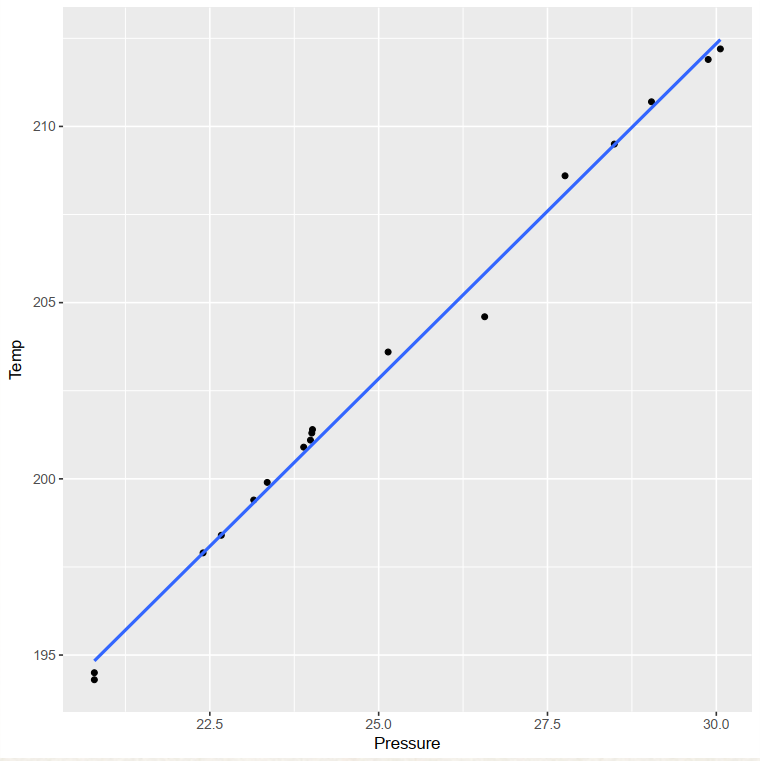
\includegraphics[width=3.8in]{forbes.png} \\
 \caption{In realistic cases, $y$ is never exactly linear in the samples $\mathbf{x}$}
\end{figure}

In such cases, $f$ is \textit{not} in  $\Hc_{reg}$. This is called \textbf{The Non-Realizable Case} in which we must  settle for finding $\hat{f} \in \Hc_{reg}$ which is "good enough" for our purposes.


\subsubsection{Geometric interpretation}

Let's denote by $\varphi_i\in \R^m$ the $i$-th row of $X$, so
    \[
 X =
\left[
  \begin{array}{ccc}
    \horzbar & \varphi_{0} & \horzbar \\
    \horzbar &\varphi_{1} & \horzbar \\
   & \vdots    & \\
   \horzbar & \varphi_{d} & \horzbar
  \end{array}
\right]
\]

In the realizable case, the system of equations $X^\Tr \mathbf{w}=\mathbf{y}$ has either a unique solution (when $dim(Ker(X^\Tr))=0$) or an infinite number of solutions ($dim(Ker(X^\Tr))\neq 0$).
In both case $\mathbf{y}\in Im(X^\Tr)$. If $dim(Ker(X^\Tr))=0$ (unique solution) then the $\varphi_0,\varphi_1,\ldots,\varphi_d$ are linearly independent.

In the non-realizable case $X^\Tr \mathbf{w}=\mathbf{y}$ has no solution so $\mathbf{y}\notin Im(X^\Tr)$.





\subsection{Designing the Learning Algorithm}

\subsubsection{The Loss Function}

To design the algorithm with which we will learn (predict) $f$ we need to choose a loss function with respect to which we will pick the "most probable" / "most likely" / "best fitting" $\hat{f}(x)$ in the linear hypothesis class $\Hc_{reg}$. We could for example choose the \textbf{Absolute Value Loss}
     \[
      L(y,\hat{f}(x)) = |y - \hat{f}(x)|
     \]
     or the \textbf{Squared Loss}
     \[
      L(y,\hat{f}(x)) = (y - \hat{f}(x))^2
     \]
There are good reasons to use each one. In this lecture \textit{we use the squared loss} since the related math is much simpler.



\subsubsection{Empirical Risk Minimization}

Since on new data we will evaluate performance by $(y-\hat{f}(x))^2$, it makes sense to choose $\hat{f}$ that minimizes that same loss $L$ \textit{on the training data we already have}.
 For a given prediction rule $\hat{f}\in\Hc$, the quantity
  \[
   \sum_{i=1}^m L(y_i,\hat{f}(x_i))\,
   \]
where $\{(\mathbf{x}_i,y_i)\}_{i=1}^m$ is our training data, is called the \textbf{empirical risk}. In our case the empirical risk of the linear function
   $\hat{f}(\mathbf{x}_i)=\mathbf{x}_i^\Tr\mathbf{w}$ is,  based on the above choice of a square-loss function, given by
   \[
   \sum_{i=1}^m(y_i-\mathbf{x}_i^\Tr\mathbf{w})^2 = \norm{\mathbf{y}-X^\Tr\mathbf{w}}^2 =
   (\mathbf{y}-X^\Tr\mathbf{w})^\Tr(\mathbf{y}-X^\Tr\mathbf{w})
   \]

\subsubsection{Least Squares}

Minimizing the empirical risk in our case means minimizing the sum of squares of the deviations of the labels from a linear function. In other words we choose the linear function in $\Hc_{reg}$ that is closest to the labels in terms of the squared error distance. The deviation $y_i-\mathbf{x_i}^\Tr \mathbf{w}$ is called the $i$-th \textbf{residual} and the total empirical risk in our case is called \textbf{Residual Sum of Squares} (or \textbf{RSS}) and is denoted by
   \[
   RSS(\mathbf{w}) = \norm{\mathbf{y}-X^\Tr\mathbf{w}}^2
   \]

\vspace{5mm}

So to learn the linear function by \textbf{Empirical Risk Minimization}, we want to find $\text{argmin} \, RSS(\mathbf{w})=\text{argmin} \norm{\mathbf{y}-X^\Tr\mathbf{w}}^2$. The empirical risk function $\norm{\mathbf{y}-X^\Tr\mathbf{w}}^2$ is a \textit{quadratic form} in $\mathbf{w}$, i.e., it is a polynomial in the $w_i$'s with terms all of degree two. It is therefore a smooth function of $\mathbf{w}$ with a minimum (or minima). If $X$ has full rank, then $\norm{\mathbf{y}-X^\Tr\mathbf{w}}^2$ has a unique minimum (as in the figure below), which we need to find in order to find $\hat{f}$.

\begin{figure}[h!]
  \centering
    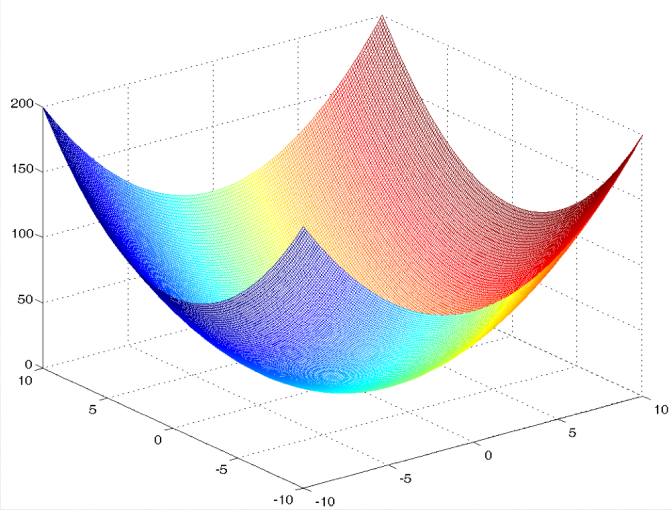
\includegraphics[width=4.5in]{parabola.png} \\
 \caption{$RSS(\mathbf{w})=\norm{\mathbf{y}-X^\Tr\mathbf{w}}^2$ in the case of $X$ with a full rank - a unique minimum}
\end{figure}

\vspace{5mm}

A \textit{necessary} condition for $\mathbf{w}$ to be a minimizer of the function $ \norm{\mathbf{y}-X^\Tr\mathbf{w}}^2$ is that all its partial derivative vanish at $\mathbf{w}$. Recalling the definition of the inner product, this condition can be written as:
    \[
    \frac{\partial}{\partial w_j} RSS(\mathbf{w}) =
    -2\sum_{i=1}^m (\mathbf{x}_i)_j \cdot (y_i-\mathbf{x}_i^\Tr \mathbf{w})=0
    \]
for all $j=0\ldots,d$, where $(x_i)_j$ is the $j$-th entry of  $\mathbf{x}_i$, that is, it is the $x_{j,i}$ element of the matrix $X$.
 We can write all these $d+1$ equations in matrix form as a linear system:
    \[
    \nabla RSS(\mathbf{w}) = -2X(\mathbf{y}-X^\Tr \mathbf{w})=0
    \]


\subsection{The Normal Equations}

So a necessary condition for $\mathbf{w}$ to be a minimizer or $RSS(\mathbf{w})$ is that $\mathbf{w}$ is a solution to the linear system
\[
 X(\mathbf{y}-X^\Tr \mathbf{w})=0
\]
or, equivalently
\[
X \mathbf{y}= XX^\Tr \mathbf{w}
\]
These are the famous \textbf{Normal Equations}, a name that will become clearer later on.


\subsubsection{Solving the Normal Equations}
Let's \textit{assume more samples than features, $m\geq d+1$}. \footnote{This is a reasonable assumption in our case if we have, say, hundreds of customer features available to us (age, sex, income, previous item purchased and so on), but thousands (or millions) of customers in our samples. There can be other cases: Suppose, for example, that the customer features contain, among other things, all previously purchased items. Now consider Amazon in Israel. The total customer pool is of the order of millions, while Amazon offers (many) millions of products. So in such a case, it may very well be that $m<d$.},




Let us also \textit{assume that the linear system $X^\Tr \mathbf{w}=\mathbf{y}$ has at least one solution}\footnote{This assumption might seem somewhat contradictory with the first one ($m\geq d+1$): The more data we collect, $m$ (which is the number of linear equations 'zipped' in $XX^\Tr \mathbf{w}=X\mathbf{y}$ ) grows, so the $d$ numbers which are represented by $\mathbf{w}$ need to satisfy more and more equations. However, many of these equations are \emph{dependent} and do not add new information to what we learn about the function $f$. In reality, the assumption that there is a (deterministic) function $f$ that we can learn and then 'know everything' is never valid (e.g., due to $f$ being too complicated and not in the hypothesis class, or due to random noise in the labels $\mathbf{y}$) and therefore, the larger $m$ is, the better $\hat{f}$ we can find.}
which implies that it either has $1$ (unique) or $\infty$ solutions. As we know from linear algebra, it has a unique solution if and only if $dim(Ker(X^\Tr))=0$, because if $Ker(X^\Tr)$ contains any vector $\mathbf{w}'\neq \mathbf{0}$, then any vector of the form $\mathbf{w}+a\mathbf{w}'$ would also be a solution.
\vspace{3mm}
Homework: Show that $dim(Ker(X^\Tr))=0$ if and only if $dim(Ker(X\cdot X^\Tr))=0$ and conclude that there exists a unique solution if and only if $X\cdot X^\Tr$ is invertible.
\vspace{3mm}


We first consider the case of a \textit{unique solution}. We would like to solve our set of equations but in order to have a procedure that is generalizable for cases in which our assumptions do not hold, and for computational reasons,  we prefer to invert matrices instead of using Gauss elimination.
$X^\Tr$ is not a square matrix and therefore is not invertible, but $X\cdot X^\Tr$ is square and because we assume a unique solution, it is also invertible we can right-away solve for $\mathbf{w}$:
\begin{eqnarray*}
  \mathbf{w} &=&  (X X^\Tr)^{-1}X\mathbf{y}
\end{eqnarray*}
So we can  learn $\mathbf{w}$, i.e., learn the linear function, simply by using the above formula.

Consider now the second case, where $dim(Ker(X\cdot X^\Tr))\neq 0$  and therefore $X\cdot X^\Tr$ is not invertible. We
 know that there is an infinite number of solutions,  since $dim(Ker(X\cdot X^\Tr))\neq 0$.
but we can not invert $X\cdot X^\Tr$. On the other hand, we do not want to use Gauss elimination because it is too \textit{numerically unstable} (more on that, soon).
Even if there is an infinite number of solutions, we still need a way to find at least one. Instead of the standard method (Gauss elimination) we all learned in linear algebra courses, in the next section we will apply an easily-generalizable and \textit{computationally-stable} technique, using the \textbf{Singular Value Decomposition} of matrices, or \textbf{SVD}.


\subsection{Singular Value Decomposition}

The \textbf{Singular Value Decomposition} or \textbf{SVD} is based on the following facts:

\begin{itemize}
  \item \textit{Any} real matrix, and in particular, our $d+1$-by-$m$ matrix $X$, can be written as
    \[
  X=U\cdot \Sigma \cdot V^\Tr
    \]

where $U$ is an orthonormal $d+1$-by-$d+1$ matrix, $\Sigma$ is a $d+1$-by-$m$ diagonal matrix, and $V$ is an orthonormal $m$-by-$m$ matrix.
For every matrix there can be many SVD's. In particular, there is an SVD where the diagonal elements of $\Sigma$,  denoted by $\Sigma_{i,i}\equiv \sigma_i$, satisfy  $\sigma_1\geq \sigma_2\geq \ldots,\geq \sigma_{d+1}\geq 0$. The $\sigma_i$'s are called the \textbf{singular values} of $X$.

  \item The columns of $U$ are eigenvectors of $XX^\Tr$. These columns are called the \textbf{left singular vectors} of $X$.
  \item The columns of $V$ are eigenvectors of $X^\Tr X$. These are called the \textbf{right singular vectors} of $X$.
  \item $\sigma_1^2,\ldots,\sigma_{d+1}^2$ are the shared eigenvalues of both $X^\Tr X$ and $XX^\Tr$.
  \item The columns of $U$ and $V$ are ordered such that the $i$-th column corresponds to the eigenvalue $\sigma_i^2$.
  This is important because the unique choice of ordering of the singular values: $\sigma_1\geq \ldots,\geq \sigma_{d+1}\geq 0$  in $\Sigma$ puts constraints on the choice of $U$ and $V$.

\end{itemize}

We stress that \textit{any} real matrix has an SVD decomposition (or a lot of them) - whether or not it is diagonalizable, or even square! This is one of the reasons why SVD is \textit{Incredibly useful} in learning and data science.

The SVD has many useful properties one of which is the following: $dim(Ker(X^\Tr))=0$ if and only if $\sigma_{d+1}>0$ (that is, all the singular values are nonzero).
So one can tell $dim(Ker)$ and $dim(Im)$ of a matrix simply by looking at its singular values.

\vspace{5mm}

Another useful property of SVD is (for proof, see homework):

Let $\Sigma^\dagger$ be a  $m$-by-$d+1$  diagonal matrix with diagonal elements
  \[
   \Sigma^\dagger_{i,i} =
   \begin{cases}
 1/\sigma_i & \sigma_i>0\\
 0 & \sigma_i=0
   \end{cases}
  \]

 We now define
    \[
  \hat{\mathbf{w}}=U (\Sigma^\dagger)^\Tr V^\Tr \mathbf{y} =(X^{\Tr})^{\dagger}\mathbf{y}
    \]


Theorem: $\hat{\mathbf{w}}$ is \emph{always} a solution to the system  $XX^\Tr \mathbf{w}=X\mathbf{y}$ independently of whether or not $X X^\Tr$ is invertible:
If $X X^\Tr$ is invertible (the case of a unique solution), then  $\hat{\mathbf{w}} = (XX^\Tr)^{-1}X\mathbf{y}$ so we recover the unique solution.
Even if $X X^\Tr$ is not invertible, that is, even if there are $\infty$  solutions to the system of equations  $XX^\Tr \mathbf{w}=X\mathbf{y}$ , $\hat{\mathbf{w}}$ is still one of them, in fact a one with a \emph{minimal norm}:
  $$\norm{\hat{\mathbf{w}}}=min\left\{ \norm{\mathbf{w}}\,:\,XX^\Tr \mathbf{w}=X\mathbf{y} \right\}$$


\vspace{4mm}
To conclude, SVD is useful for learning $\mathbf{w}$ because, among other things, it  works regardless of whether there are $1$ or $\infty$ solutions.
Another major reason why SVD is useful for learning is because it is \emph{numerically stable}, as explained below.

\subsubsection{Making the SVD solution numerically stable}

Computers don't calculate over $\R$, they use bits and more specifically they use floating-point arithmetics with very finite precision. A lot of non-trivial knowledge and care are required in order to understand how learning algorithms are actually implemented in software.\textit{Any} learning algorithm comes down to a lot of calculus (e.g gradients) and linear algebra (e.g. inverses) implemented in software. You should care \textit{deeply} about how algorithms are implemented and when they break numerically, as in the following example.
\vspace{5mm}

Sometimes $XX^\Tr$ is formally invertible but \textit{close to singular}. This happens if columns of $X^\Tr$ are \textit{almost} co-linear or if one column of $X^\Tr$ is \textit{almost} spanned by other columns. In this case some singular values of $X$ will be nonzero, but very small. When this happens, Gauss elimination may yield wildly incorrect results. Also, because of double-precision arithmetics, $1/\sigma_i$ will not be precise. The practical solution in such cases is to choose a \textbf{machine precision threshold}, $\varepsilon$ and let
\[
  \Sigma^{\dagger,\varepsilon}_{i,i} =
                           \begin{cases}
                             1/\sigma_i & \sigma_i>\varepsilon\\
                             0 & \sigma_i \leq \varepsilon
                           \end{cases}
                         \]




\subsection{How many samples do we need to learn a linear function?}
The system $X^\Tr \mathbf{w}=\mathbf{y}$ has $m$ equations in $d+1$ variables. If $m<d+1$ we have no hope of learning $f$ - we don't have enough data.
Our hypothesis class is a $d+1$-dimensional linear space: the larger $d$, the more complicated the hypothesis space. So the larger $d$, the more samples we need to learn it.


\subsection{Summary - Noiseless Case}
Before presenting a concrete example, let us summarize what we discussed so far about learning linear functions. When the training data is $(\mathbf{x},f(\mathbf{x}))$ with $f$ a linear function, we know how to learn $f$. We need at least $d+1$ training samples. We learn by solving the system $XX^\Tr \mathbf{w}=X\mathbf{y}$. This can be done in a numerically stable way using the SVD, regardless of whether or not the system has a unique solution or not.
If there is a unique solution, SVD recovers it and in that case, this is the same solution we would get by simply inverting $XX^\Tr$ and multiplying both sides of the normal equations by that inverse.
If there are infinitely many solutions, SVD will recover one which has a minimal norm.


\section{The Linear Model - Noisy Case }

As we mentioned before, the assumption that the labels $y$ are \textit{exactly} linear in the samples $\mathbf{x}$ is not realistic. The deviation from linearity can happen simply because the real deterministic function, $f$, is only approximately linear, but also because that $f$ is obscured by random inaccuracies in the values of the samples, the labels or both. This is the case we would like to discuss.

\subsection{Data Generation Model With Noise}

So far we assumed that training data is created by a deterministic process\footnote{We recall that by "Deterministic" we simply mean: if the same $\mathbf{x}$ appears again, it appears with the same $\mathbf{y}$.}, that is, there exits a function $f(x)$ where the training data is of the form
 \[
  \Big(x_i \,,\, f(x_i)\Big) \qquad i=1,\ldots m
 \].

We now would like to consider a more general and much more realistic case where the training data is of the form
  \[
  \Big(x_i \,,\, f(x_i) + z_i \Big) \qquad i=1,\ldots m
 \]

with $z_1,\ldots z_m\iid (0,\sigma^2)$ , meaning that the noise generated by i.i.d random variables from some distribution with mean $0$ and variance $\sigma^2$. So from now on, our treatment of learning will be probabilistic: Due to the random noise, even for identical $\mathbf{x}$'s, we may end up with different $y$'s. In order to be able to learn we therefore adapt what we did so far in the deterministic case to the probabilistic (noisy) one.

Let us still assume the linear hypothesis class and that we have enough data to learn, namely $m\geq d+1$. So, as before, there is an unknown $\mathbf{w}$ such that for every sample vector $\mathbf{x}_i$ in our data (that is, every column in our data matrix $X$):


$$y_i=\mathbf{x}_i^\Tr \mathbf{w}+z_i$$


Denoting the noise vector $\mathbf{z}=(z_1,\ldots,z_m)^\Tr$ we have in matrix notation
$$\mathbf{y}=X^\Tr\mathbf{w}+\mathbf{z}$$.

Note that the vector $\mathbf{y}$ is no longer necessarily \footnote{Unless, by an extreme accident, $\mathbf{z}\in Im(X^\Tr)$. Moreover, due to the noise term, for the \textit{same} $\mathbf{x}$, one can have two \textit{different} $y$'s, which \textit{guarantees} that there will be no solution} in $Im(X^\Tr)$ in which case the system $\mathbf{y}=X^\Tr \mathbf{w}$ has no solutions.



\begin{figure}[h!]
  \centering
    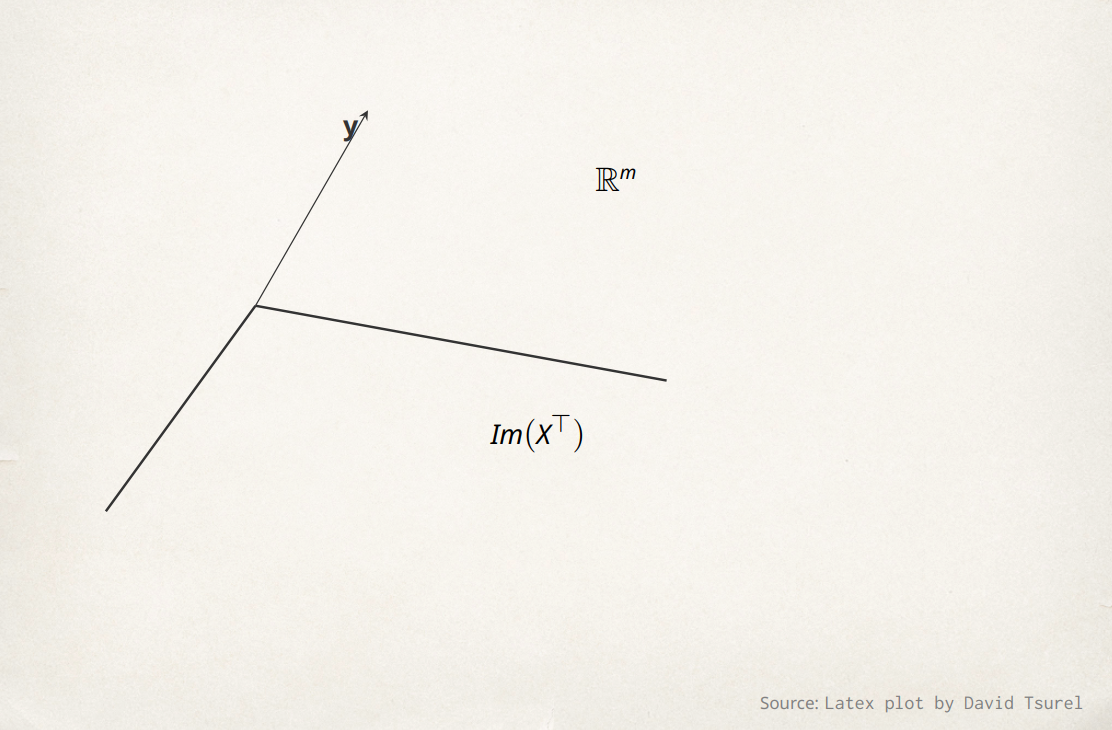
\includegraphics[width=4.5in]{PlotTsurel.png} \\
 \caption{$\mathbf{y}$ no longer in $Im(X^\Tr)$}
\end{figure}



 Let's use the square loss function as before, and learn by empirical risk minimization:
         \[\mathbf{w}_S := \text{argmin}_{\mathbf{w}}\norm{y - X^\Tr \mathbf{w}}
         \]
        This means learning $h_S\in\Hc_{lin}$ by solving the normal equations. This makes a lot of sense.  We have
         $\mathbf{y}\notin Im(X^\Tr)$ - because the noise "pushed" $\mathbf{y}$ out of $Im(X^\Tr)$. As we've seen, solving the normal equations is equivalent to
         projecting $\mathbf{y}$ back onto $Im(X^\Tr)$ (through finding a Least Squares approximation).


\begin{figure}[h!]
  \centering
    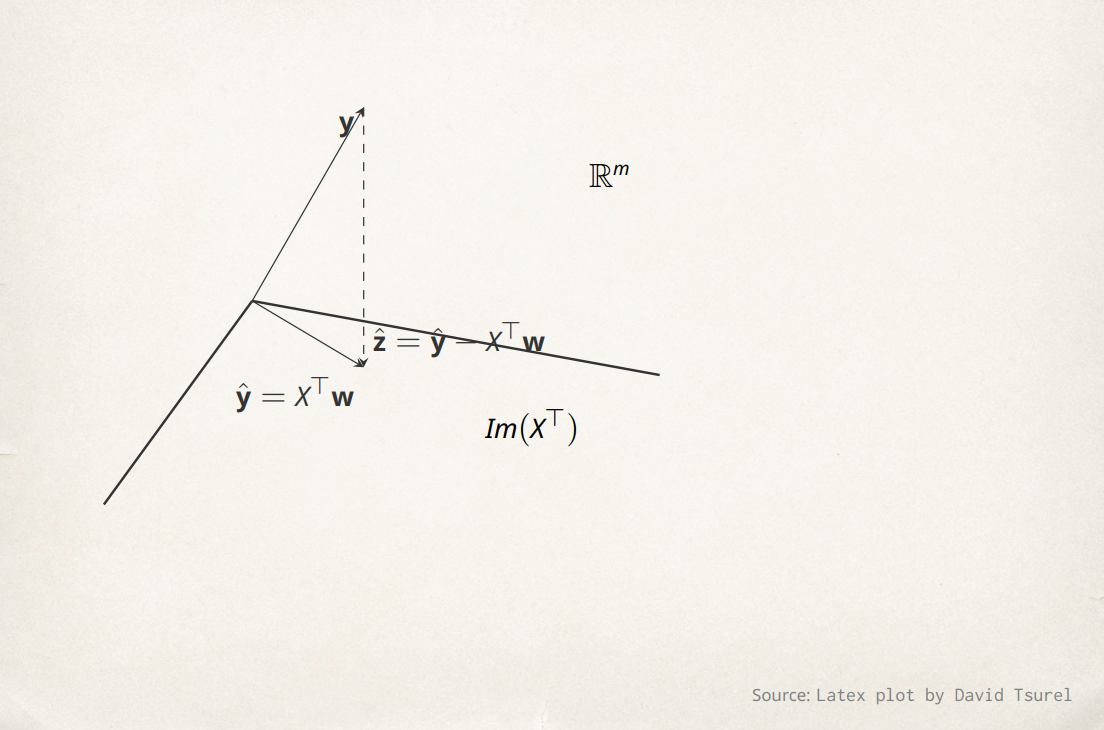
\includegraphics[width=5.5in]{Geometry2.png} \\
 \caption{$\hat{y}\equiv X^\Tr \hat{w}$ is the projection of $\mathbf{y}$ onto $Im(X^\Tr)$}
\end{figure}





\subsection{The Maximum Likelihood Principle}
 Assume further - for just a moment - that noise is Gaussian: $z_i\iid\Nc(0,\sigma^2)$. This means that the $i$-th observation is independently distributed $y_i\sim \Nc(\mathbf{x}_i^\Tr \mathbf{w},\sigma^2)$.
Suppose we {\bf knew} the weight vector $\mathbf{w}$, we could then ask the following question: The data matrix $X$ is fixed. Given that we know
          $\mathbf{w}$, what is the probability to observe a responses vector $\mathbf{y}$?

Answer: The probability density is a product of Gaussian densities:
          \[p(\mathbf{y}|\mathbf{w}) = \prod_{i=1}^m \left[ \frac{1}{\sqrt{2\pi
            \sigma^2}} e^{-\frac{(\mathbf{x}_i^\Tr \mathbf{w}-y)^2}{2\sigma^2}}\right]
          \]

This is a question in probability: We know $\mathbf{w}$, what's the chance to observe $\mathbf{y}$? But we are actually interested here in the reverse question: we sampled
$\mathbf{y}$, what's the most "likely" value of $\mathbf{w}$?

The answer is known as the {\bf Maximum Likelihood} (ML) principle which suggests: let's choose $\mathbf{w}$ for which the probability density of getting the observed $\mathbf{y}$ is maximal.
We write the {\bf likelihood function} - now a function of  $\mathbf{w}$, for fixed $\mathbf{y}$ the likelihood is
          \[
            L(\mathbf{w}\, |\, \mathbf{y}) = \frac{1}{(2\pi \sigma^2)^{m/2}}
            \prod_{i=1}^m \left[ e^{-\frac{(\mathbf{x}_i^\Tr \mathbf{w}-y)^2}{2\sigma^2}}\right]
          \]
\textbf{The Maximum Likelihood Estimator} (MLE) for $\mathbf{w}$ is thus
          \[
            \hat{\mathbf{w}}:=\text{argmax}_\mathbf{w} L(\mathbf{w}\, |\, \mathbf{y}) =
            \text{argmax}_\mathbf{w} \log L(\mathbf{w}\, |\, \mathbf{y}) =
            \text{argmin}_\mathbf{w} \sum_{i=1}^m(\mathbf{x}_i^\Tr \mathbf{w} -y_i)^2
          \]
This, by now, should look familiar: The MLE (assuming Gaussian noise) is just the Least Squares estimator we obtained by empirical risk minimization of square error loss.


\subsection{Noise, Bias and Variance}

Let us consider a concrete example of what we learnt so far.

\subsubsection{Polynomial fitting}

Consider the following special case called polynomial fitting\footnote{In spite of the term "Polynomial fitting", and the form of $\Hc$, this model is in fact a specific case of the Linear Model.
This is because we do \emph{not} require the $d$ features that we discussed in previous sections to be independent of one another}:
We are given points $a_1,\ldots a_m\in \R$  and labels $y_1,\ldots,y_m$.
We would like to learn a polynomial function $\R\to\R$ from the following Hypothesis class:
                \[
                  \Hc^d=\left\{ a\mapsto  \sum_{k=0}^d w_k a^k \right\}
                \]
 Denoting $\mathbf{x}_i=(1,a_i,a_i^2,\ldots,a_i^d)$, our hypothesis class is simply
                $\left\{ \mathbf{x}\mapsto \mathbf{x}^\Tr \mathbf{w}  \,|\,
                \mathbf{w}\in\R^{d+1}\right \}$
The matrix $X$ in this case is the \textbf{Vandermonde matrix} that you are probably familiar with from linear algebra courses. Since the $a_i$'s are different from one another, it has full rank:
$d+1$ if $d+1\leq m$ and $m$ if $d+1> m$.



\subsubsection{Polynomial fitting: no noise}
    In the following figures we chose $a_1,\ldots,a_{30}$ (horizontal values of red circles). We then chose a "true" polynomial $p$ (shown in blue curve) of degree 29 and calculated its values at these points - see the red
    circles. To fit a polynomial of degree $d$ we used linear regression on the training data $\mathbf{x}_i=(1,a_i,a_i^2,\ldots,a_i^d)$ and $y_i=p(a_i)$,  $i=1,\ldots,30$. The linear regression chose coefficients for polynomial $\hat{p}$ of degree $d$. The fitted polynomial is shown in the green curve. We evaluated the fitted polynomial $\hat{p}$ on the training data $a_1,\ldots,a_{30}$ (green circle).

 The hypothesis class in each slide consists of polynomials up to a given degree, indicated on the title. So the hypothesis class grows from slide to slide.

\newpage
\begin{figure}[h!]
\centering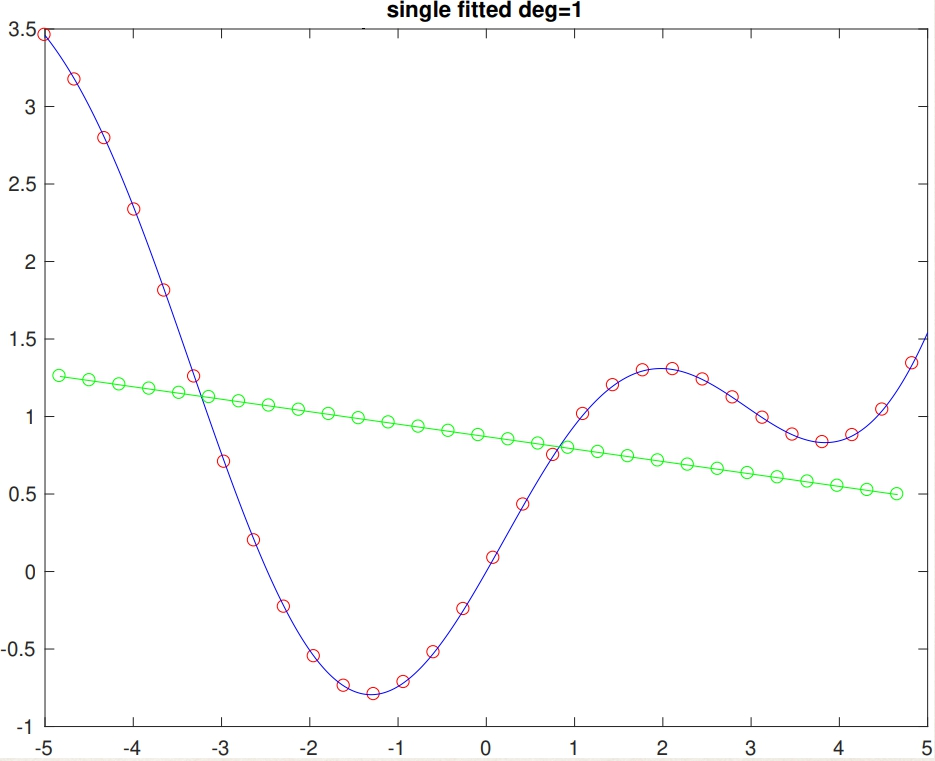
\includegraphics[scale=0.3]{clean_poly_d_1.png}
\end{figure}


\begin{figure}[h!]
\centering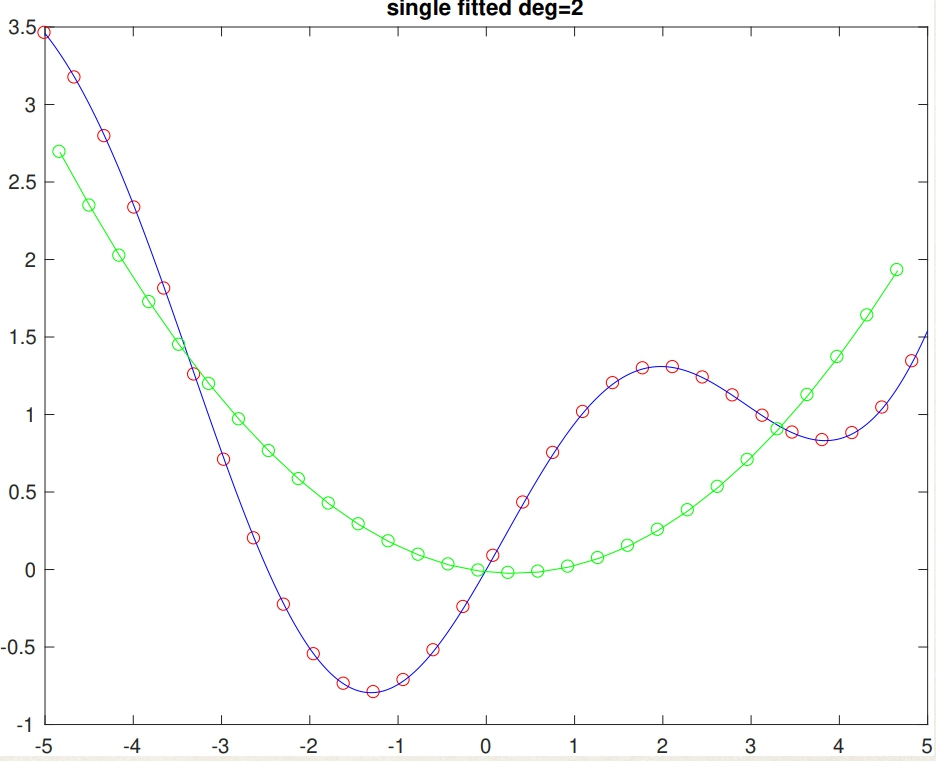
\includegraphics[scale=0.3]{clean_poly_d_2.png}
\end{figure}

\begin{figure}[h!]
\centering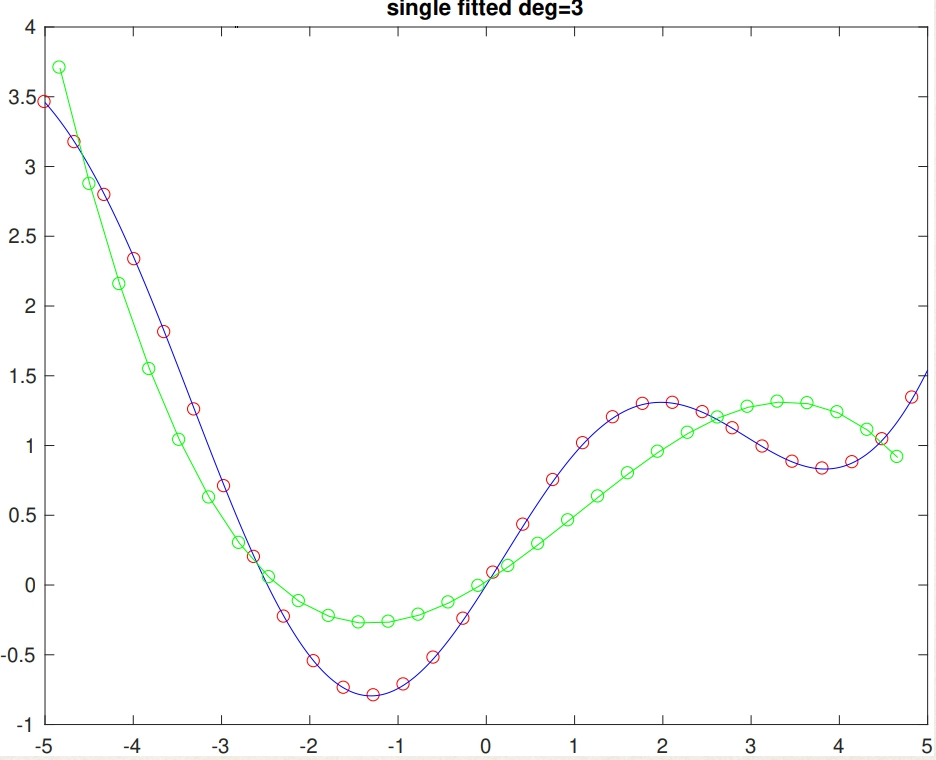
\includegraphics[scale=0.3]{clean_poly_d_3.png}
\end{figure}


\begin{figure}[h!]
\centering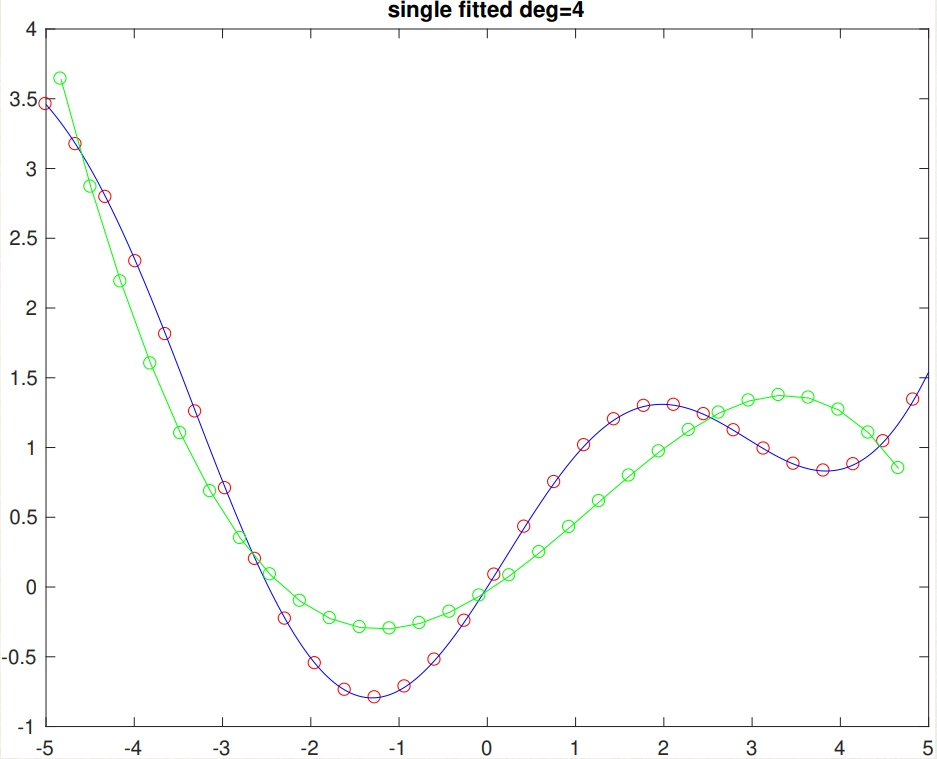
\includegraphics[scale=0.3]{clean_poly_d_4.png}
\end{figure}


\begin{figure}[h!]
\centering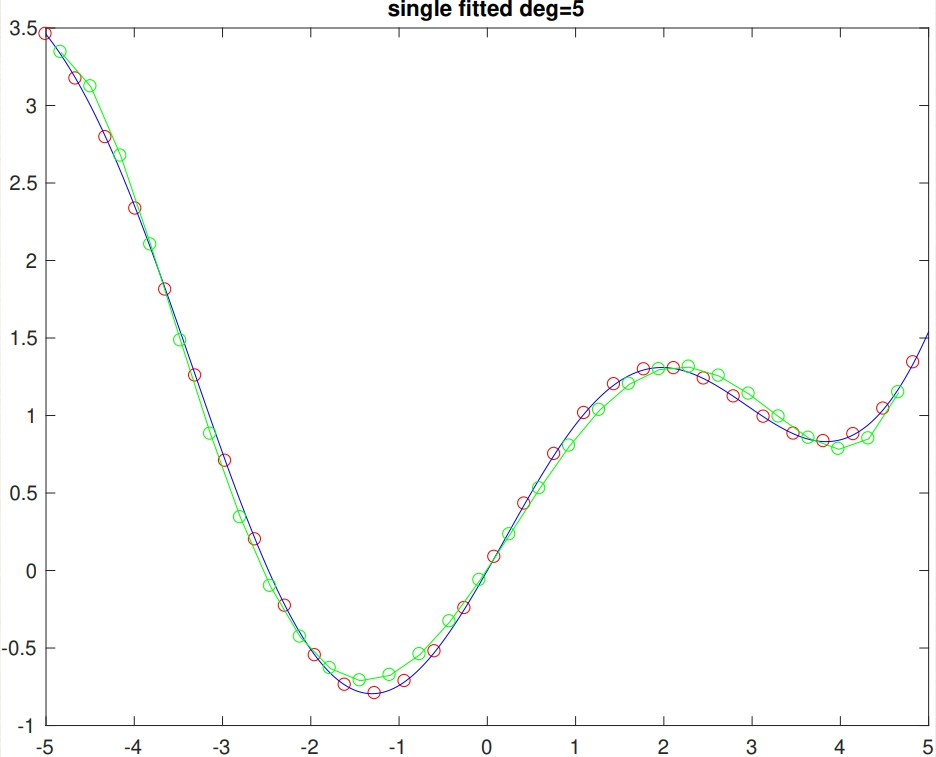
\includegraphics[scale=0.3]{clean_poly_d_5.png}
\end{figure}


\begin{figure}[h!]
\centering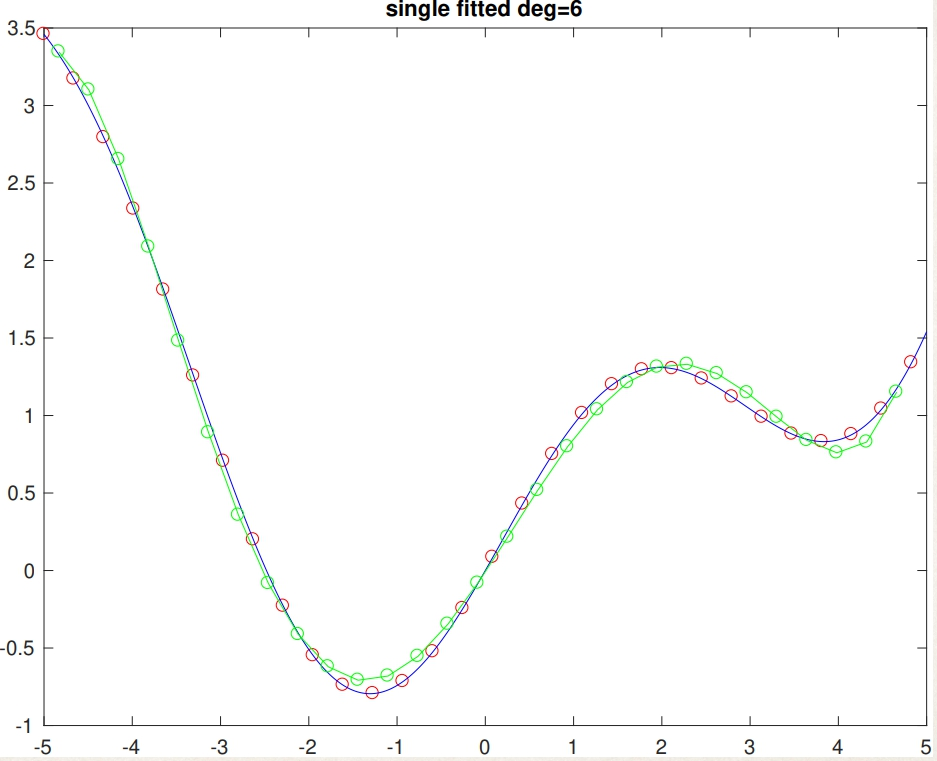
\includegraphics[scale=0.3]{clean_poly_d_6.png}
\end{figure}


\begin{figure}[h!]
\centering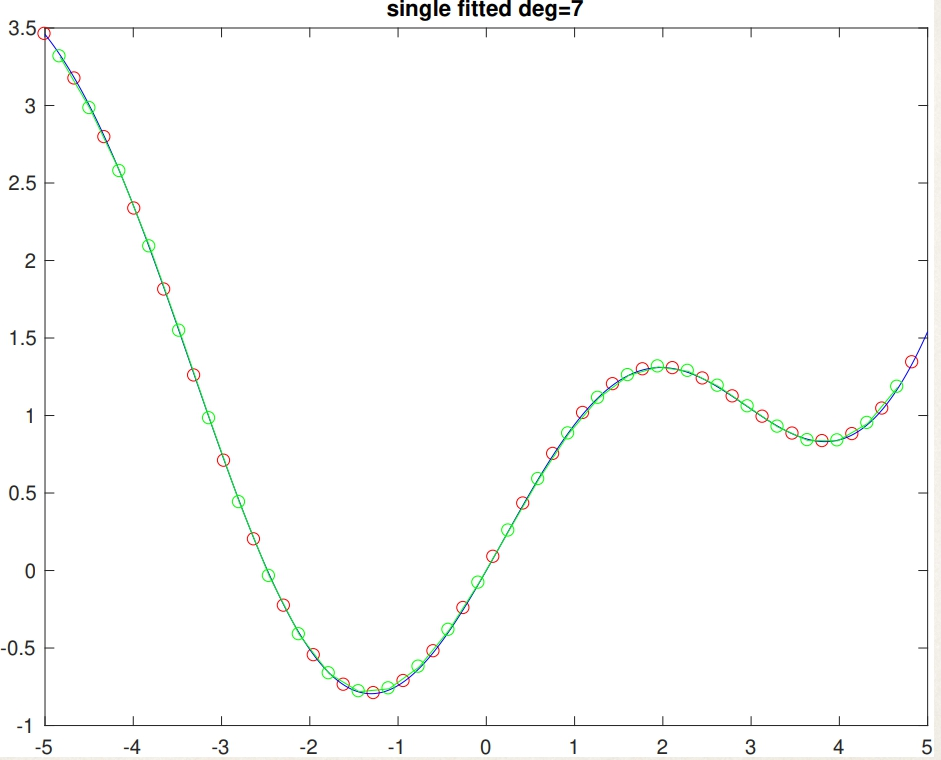
\includegraphics[scale=0.3]{clean_poly_d_7.png}
\end{figure}


\begin{figure}[h!]
\centering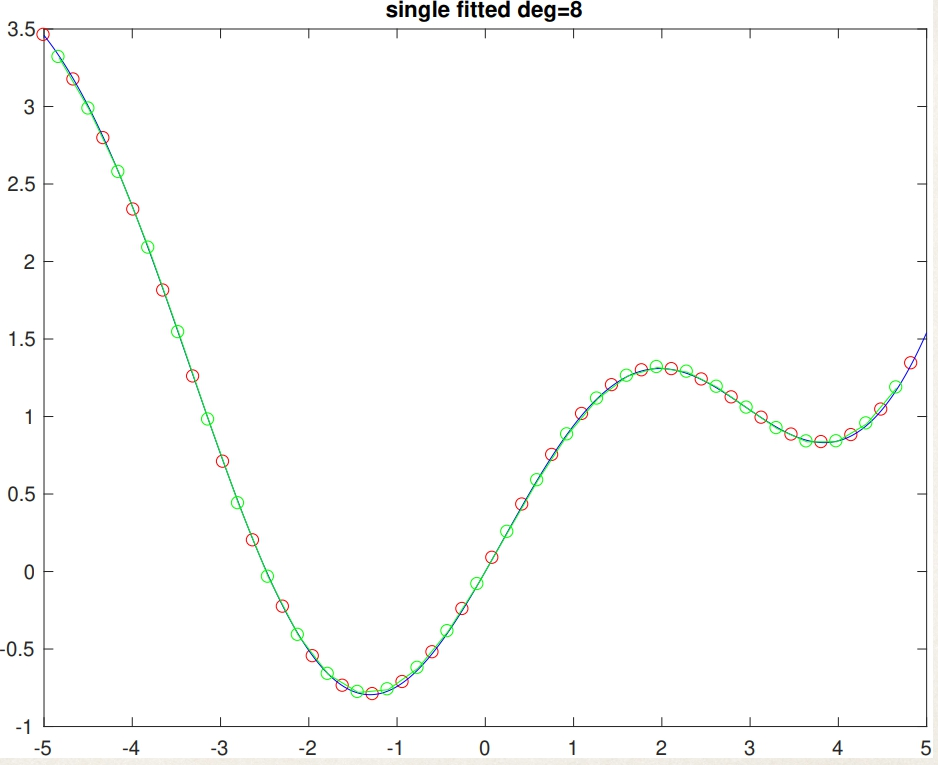
\includegraphics[scale=0.3]{clean_poly_d_8.png}
\end{figure}

\newpage

\subsubsection{Bias}
 What can we learn from these figures? For small $d$, the hypothesis class $\Hc^d$ is too small. The true polynomial $p$ of degree 29 cannot be described even by the "best approximation" to $p$
 from $\Hc^d$. Informally, {\bf Bias} describes how well the "true" $f$ can be approximated by our hypothesis class. Informally, the larger the hypothesis class, the smaller the bias.


\subsection{Polynomial fitting: with noise}
The next figures shows an evaluation of $p$ on the red  circles {\bf and added i.i.d Gaussian noise $z_1,\ldots,z_{30}\iid  \Nc(0,4)$}. The noisy values are shown in pink stars.
To fit a polynomial of degree $d$ we used linear regression with  training data $\mathbf{x}_i=(1,a_i,a_i^2,\ldots,a_i^d)$ and $y_i=p(a_i)+z_i$, $i=1,\ldots,30$.
The linear regression chose coefficients for polynomial $\hat{p}$ of degree $d$. The fitted polynomial is shown in green curve. We evaluated the fitted polynomial $\hat{p}$ on the training data $a_1,\ldots,a_{30}$ (green circle). We repeated this for several "monte carlo" iterations (different random seeds = different noise vectors). Each iteration has a different number shown on top. The only difference between slides (for same fitted degree $d$) is the noise vector

\newpage


\begin{figure}[h!]
\centering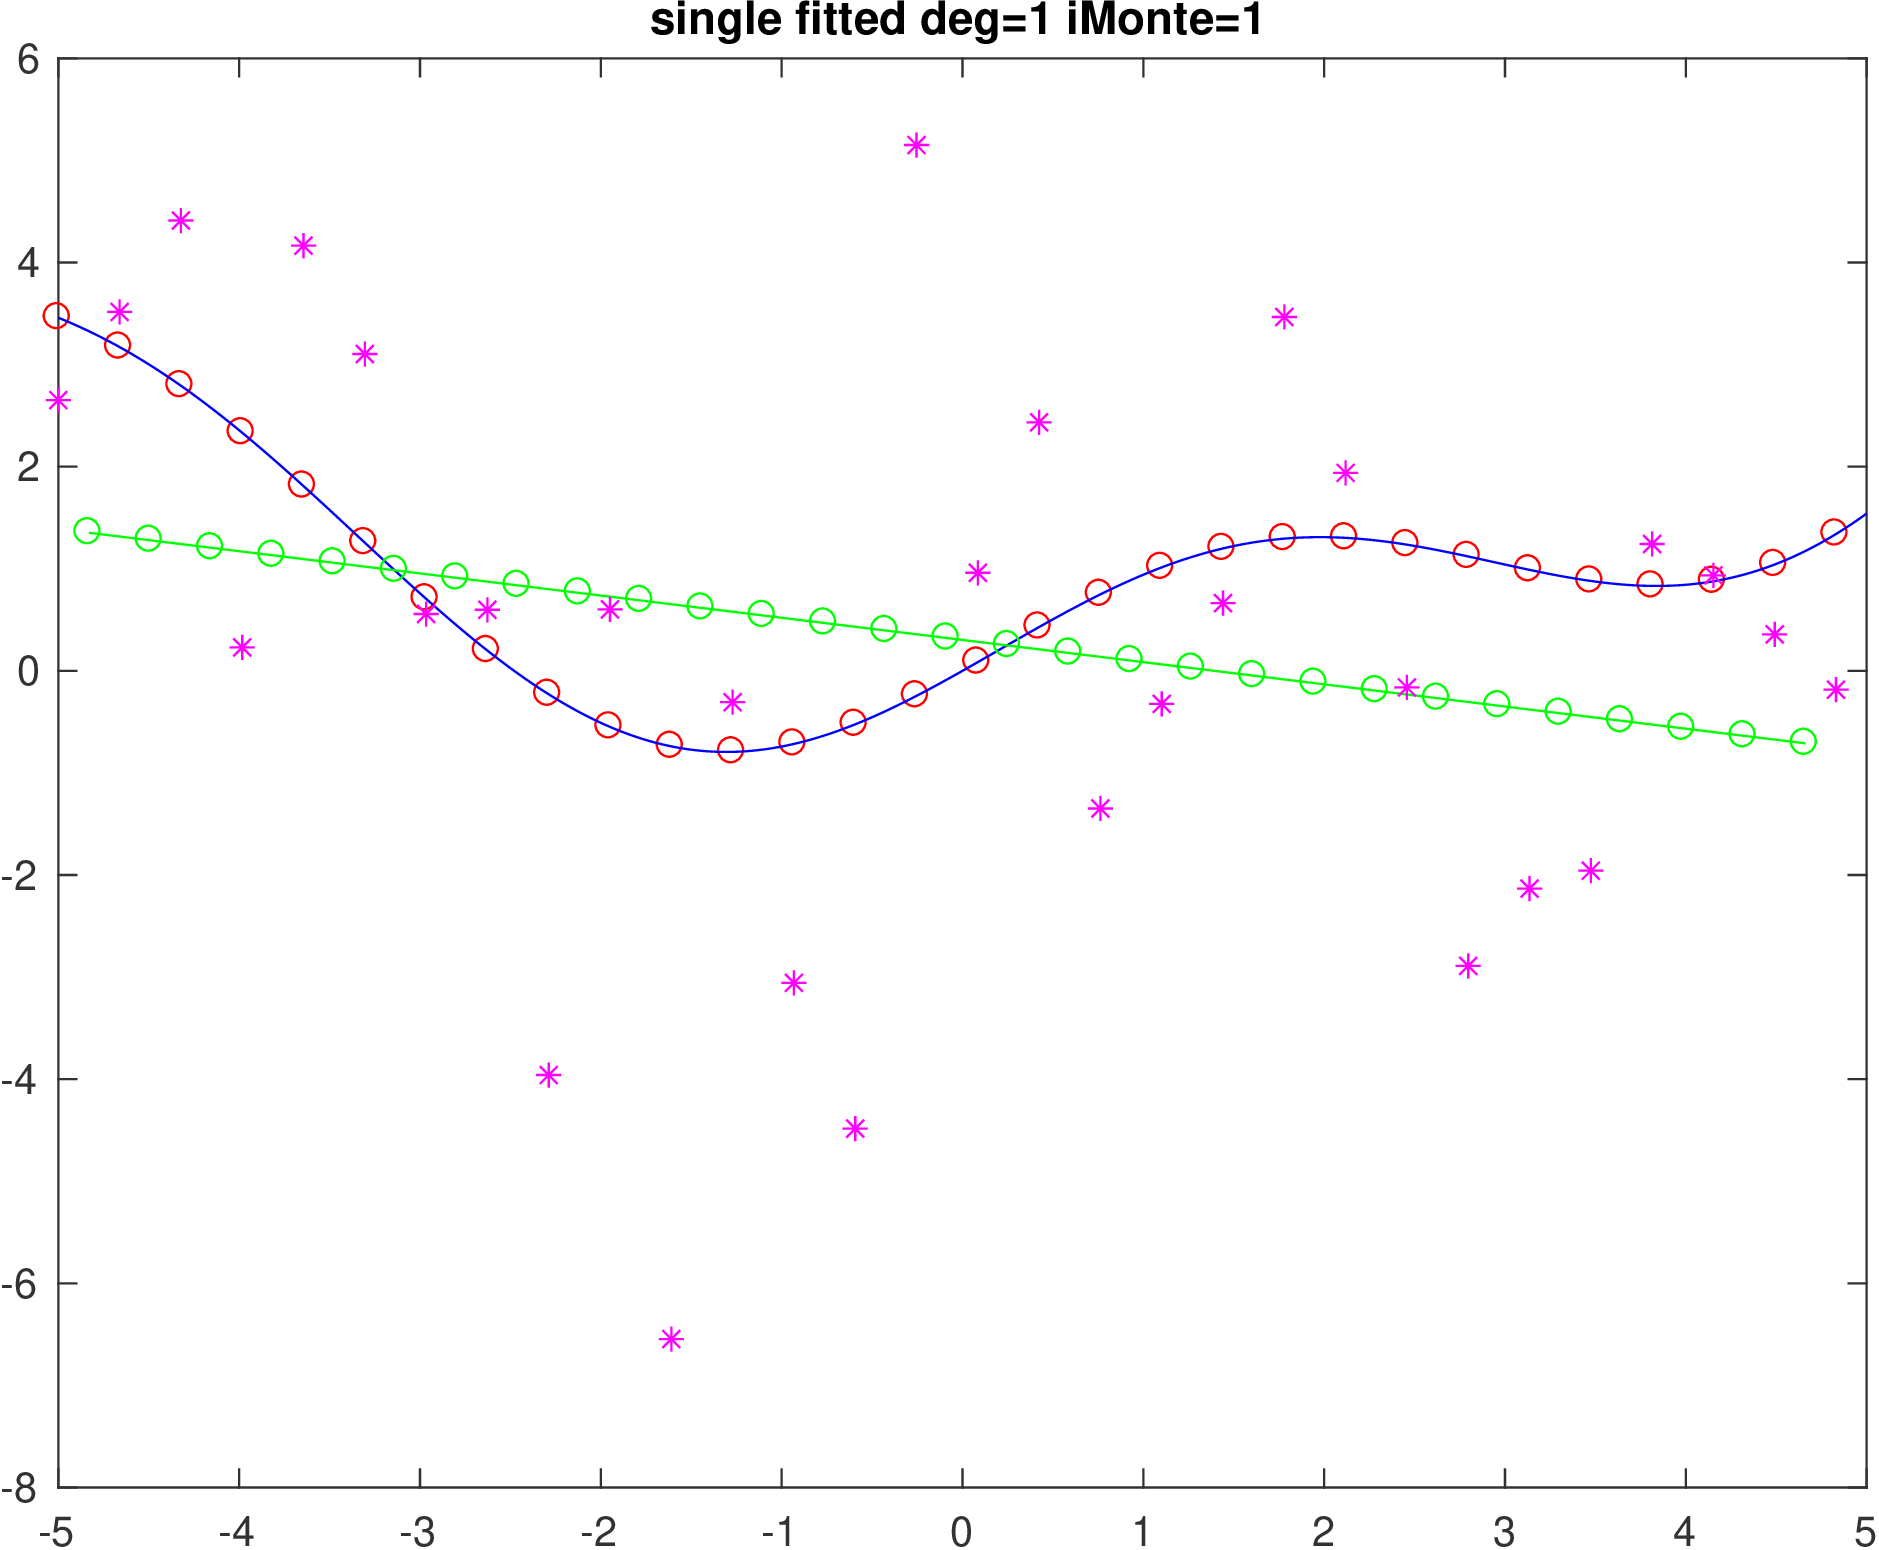
\includegraphics[scale=0.1]{single_poly_d_1_iMonte_1.png}
\end{figure}

 \begin{figure}[h!]
\centering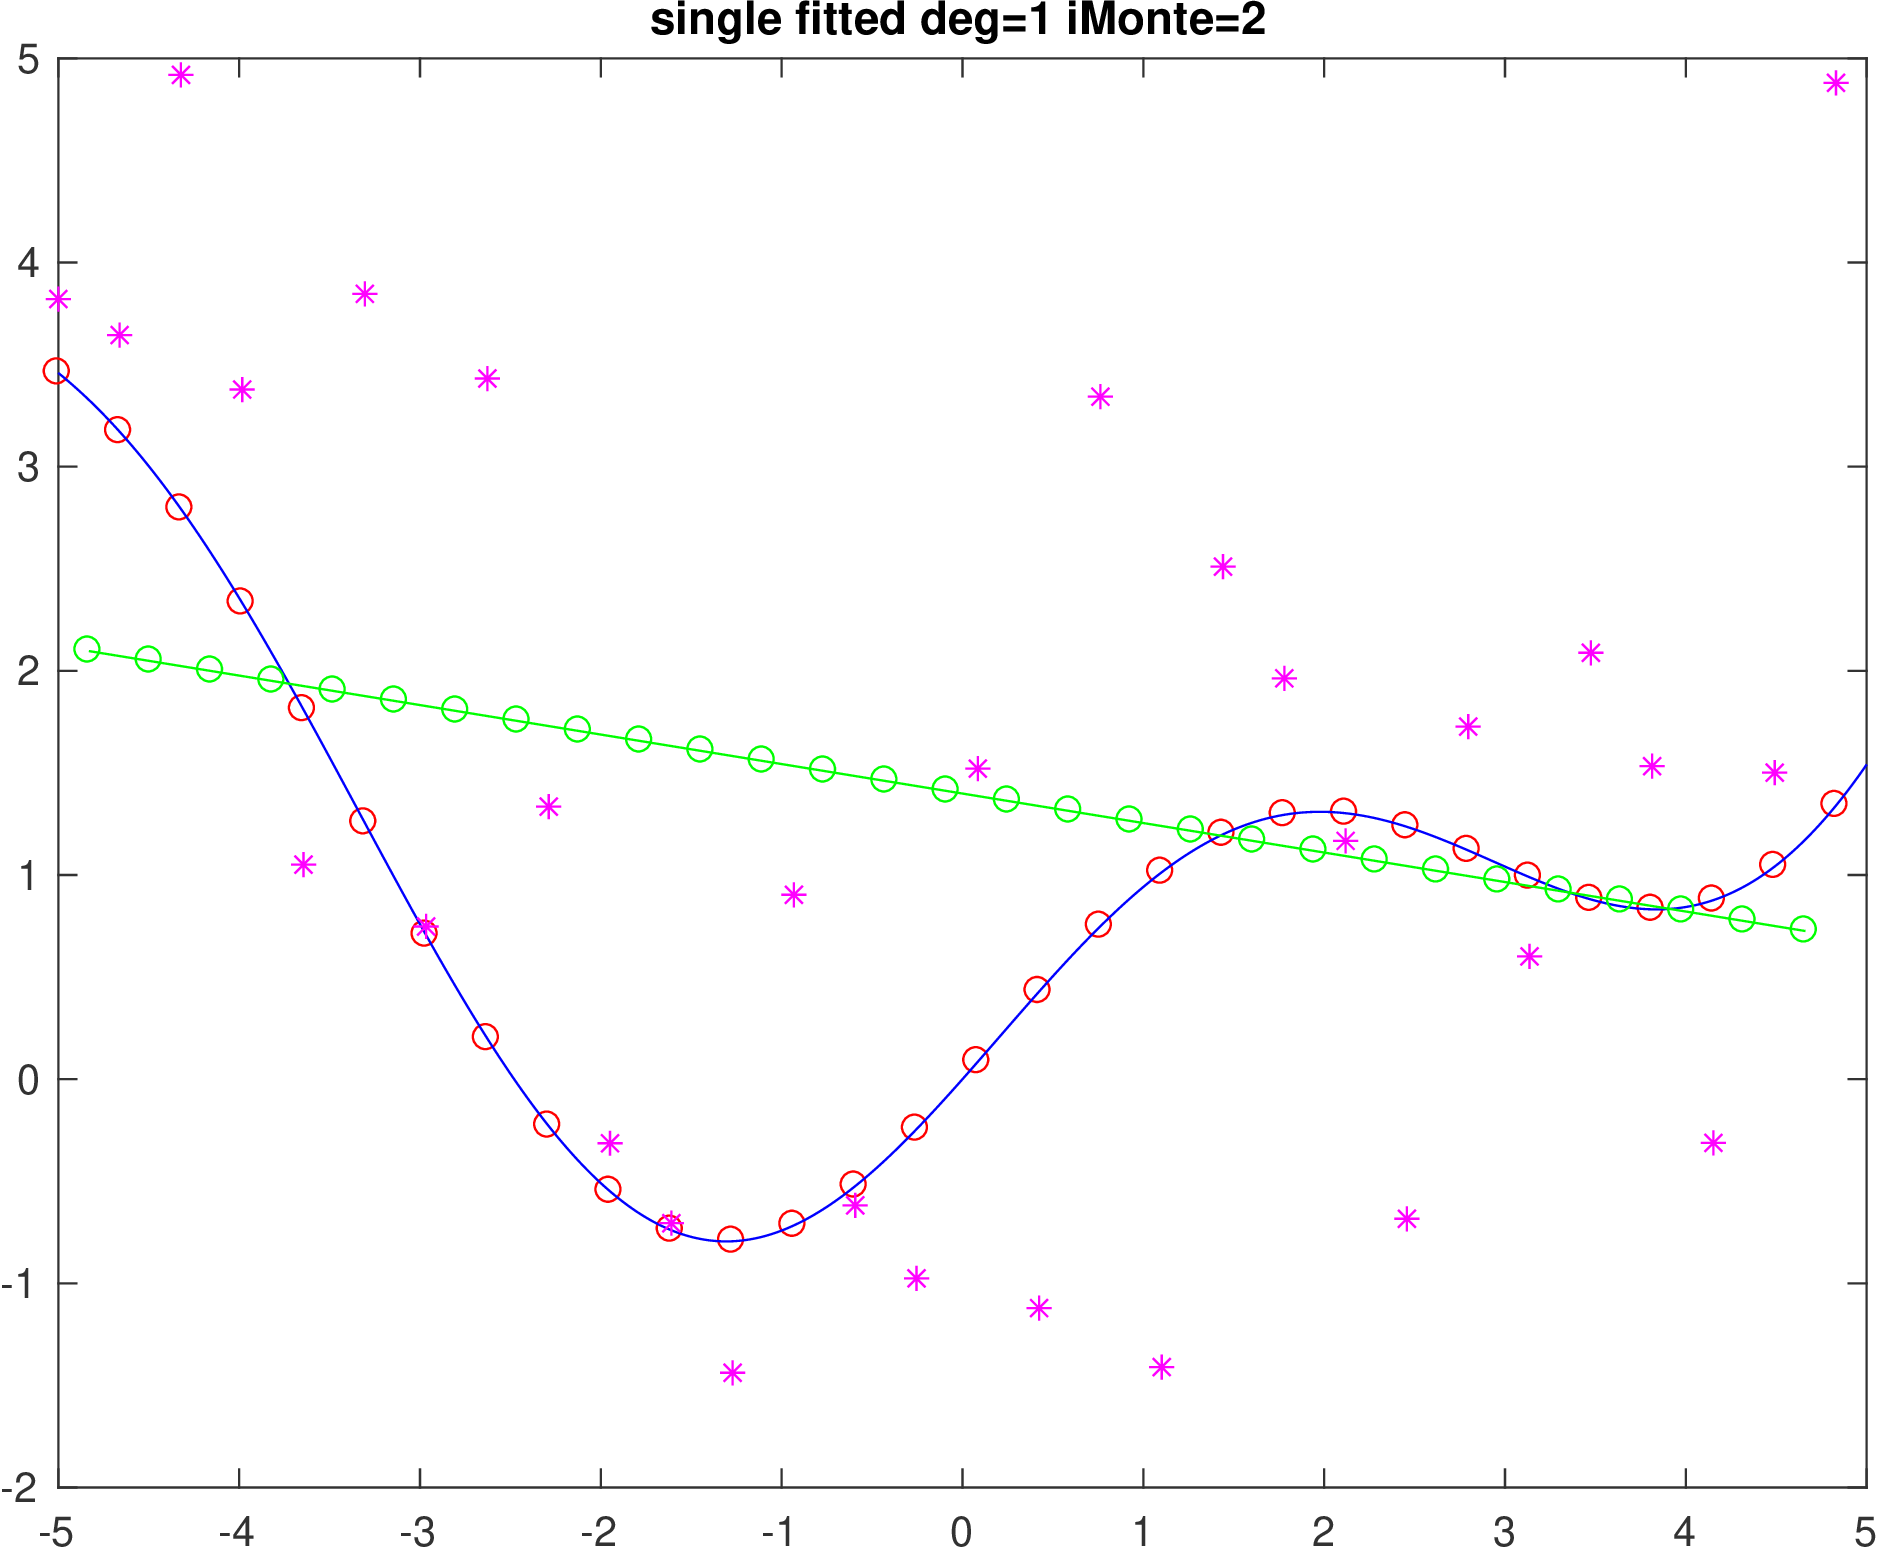
\includegraphics[scale=0.1]{single_poly_d_1_iMonte_2.png}
\end{figure}

\begin{figure}[h!]
\centering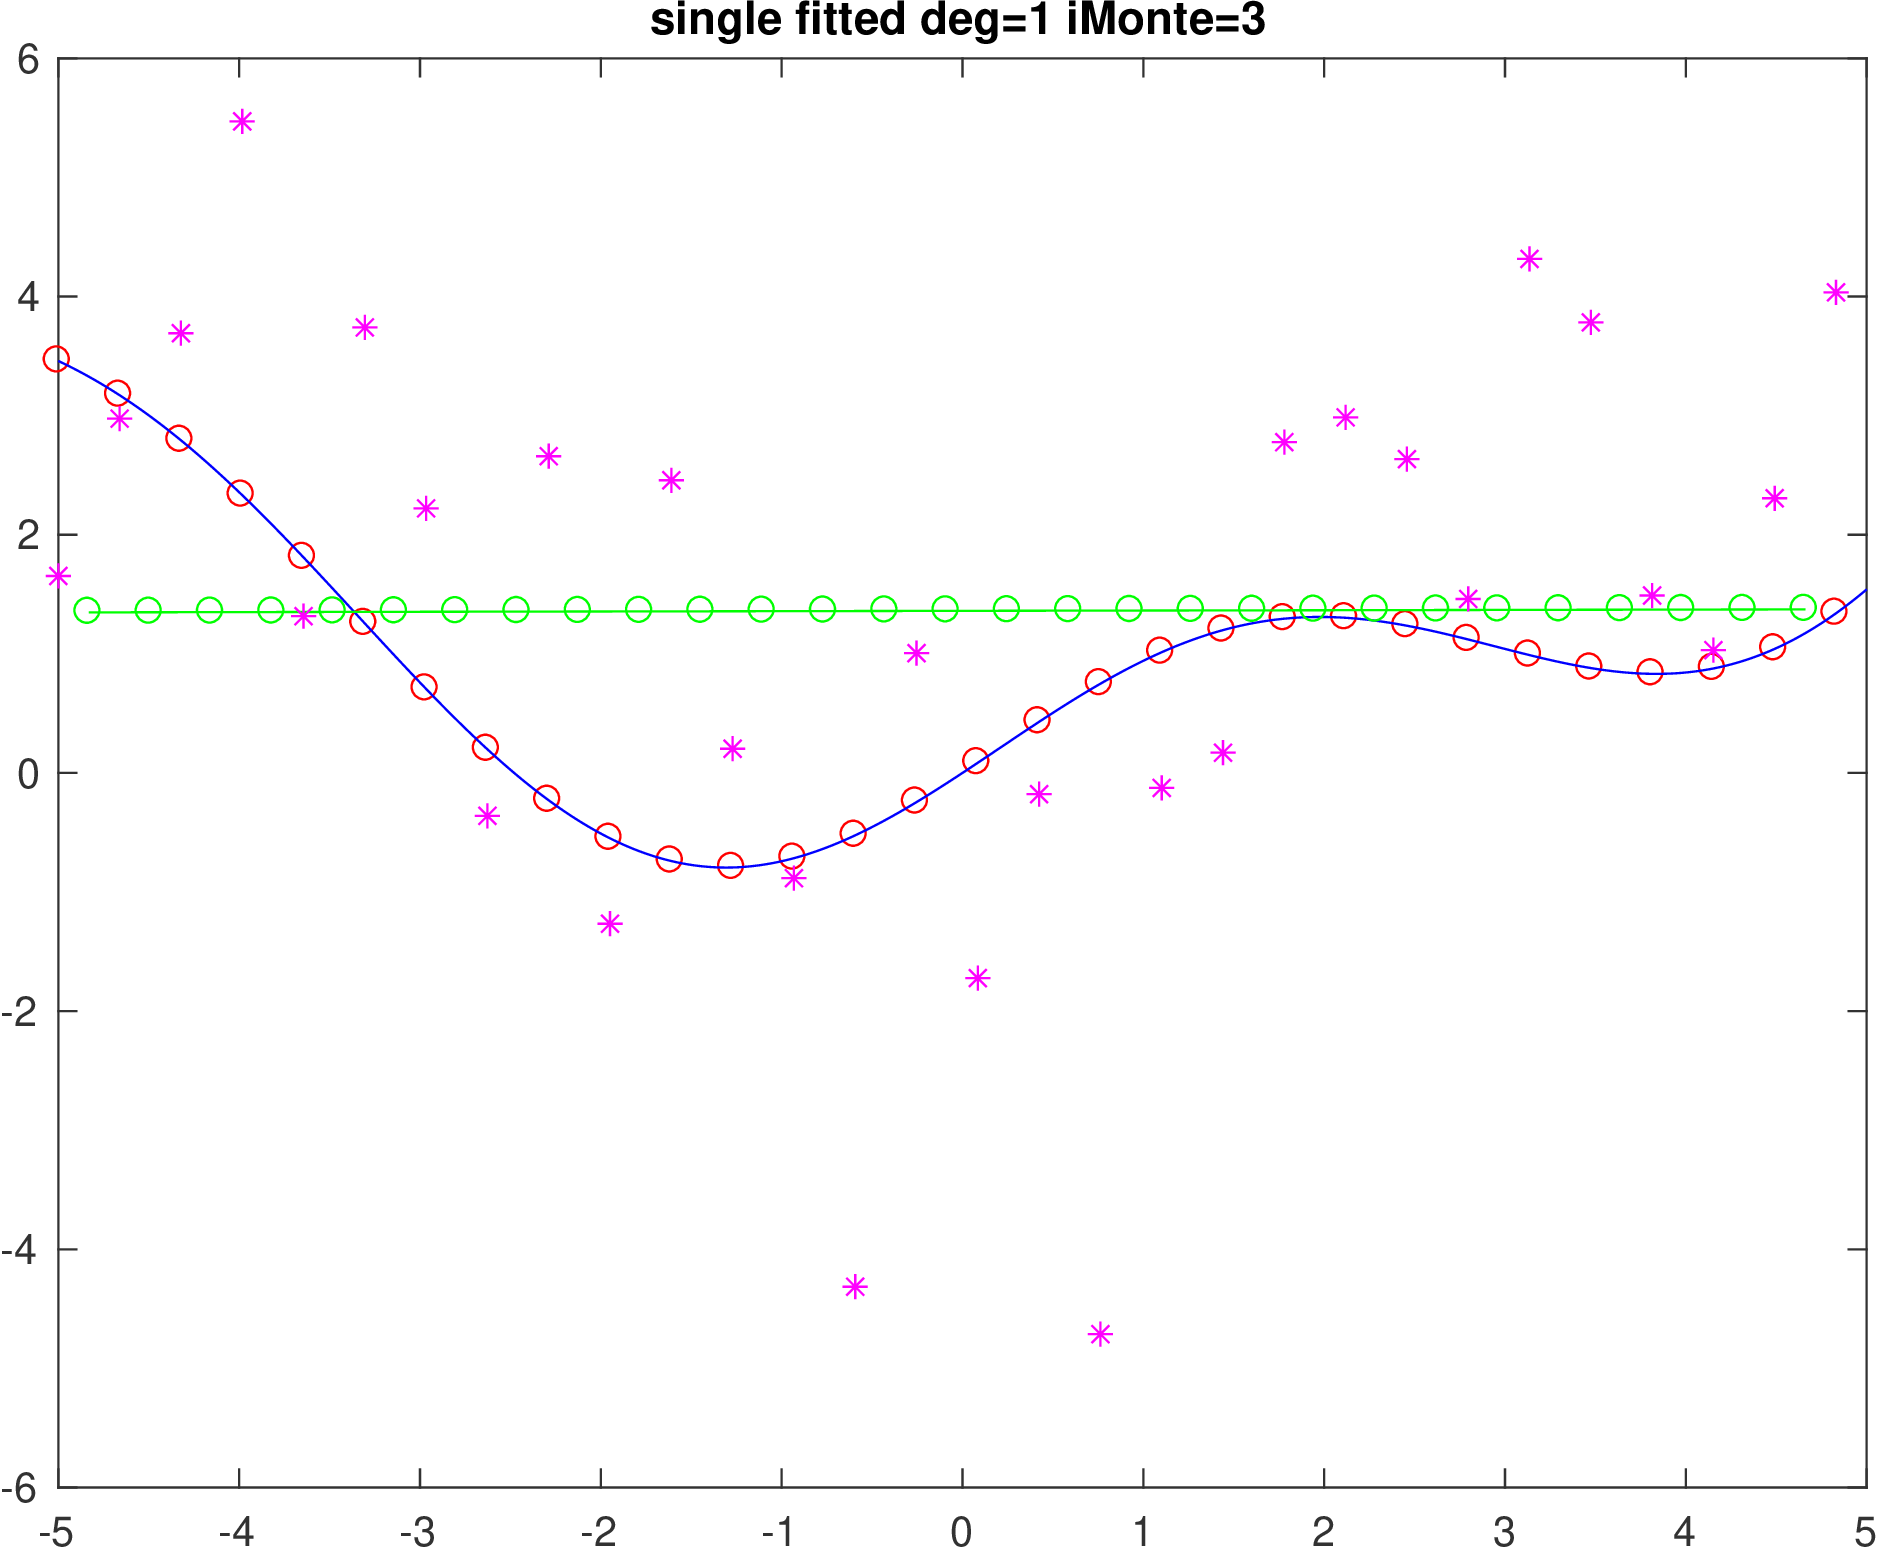
\includegraphics[scale=0.1]{single_poly_d_1_iMonte_3.png}
\end{figure}

\begin{figure}[h!]
\centering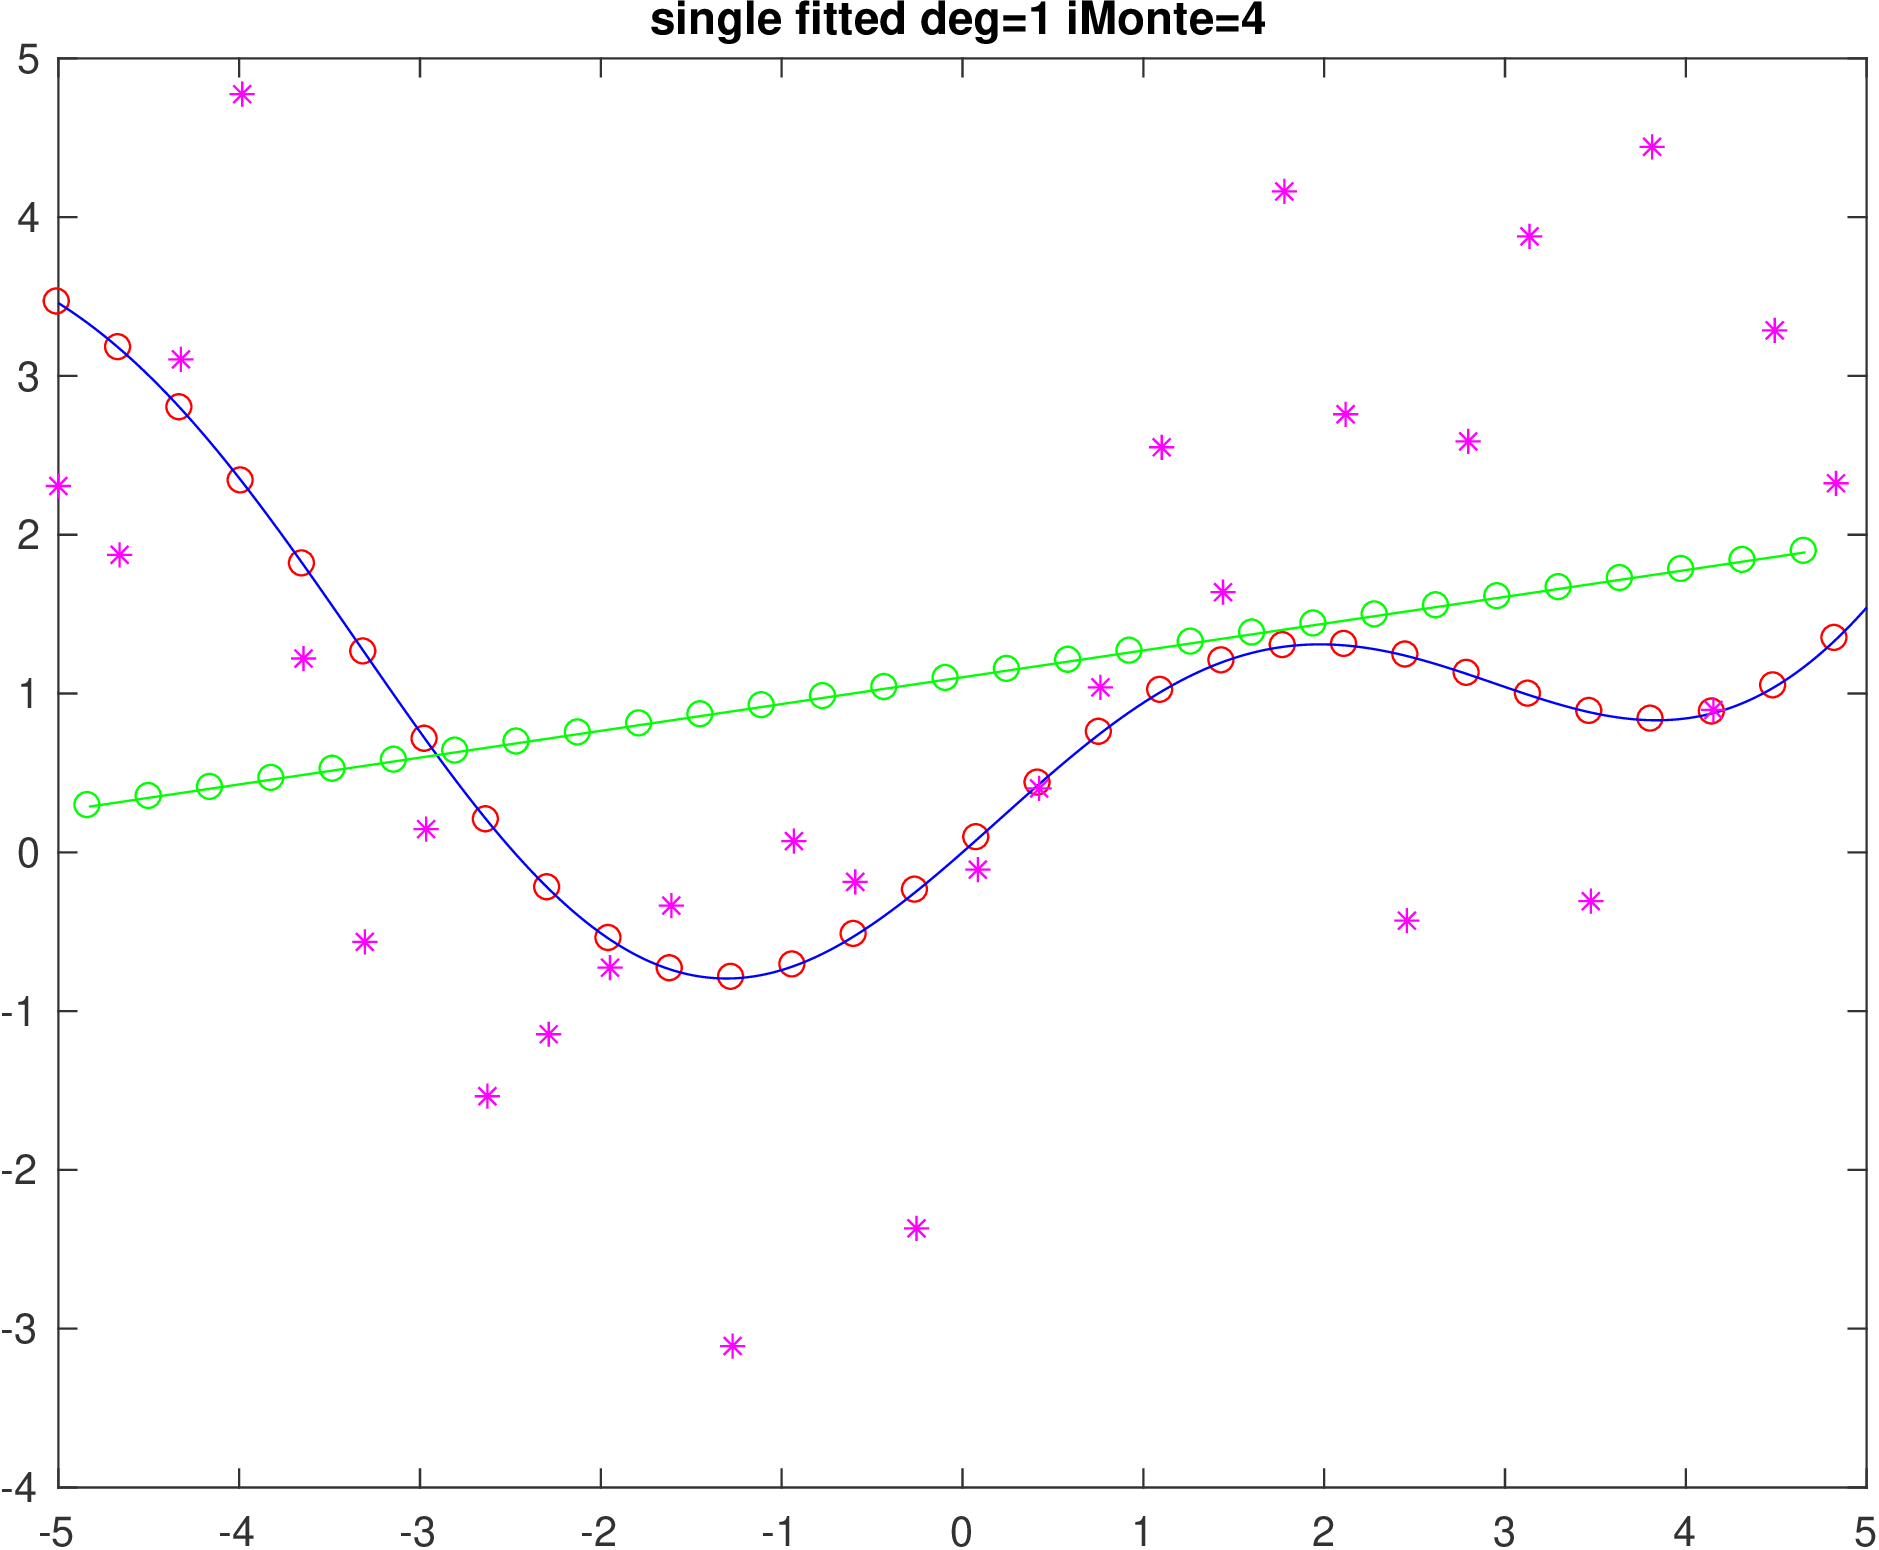
\includegraphics[scale=0.1]{single_poly_d_1_iMonte_4.png}
\end{figure}


\begin{figure}[h!]
\centering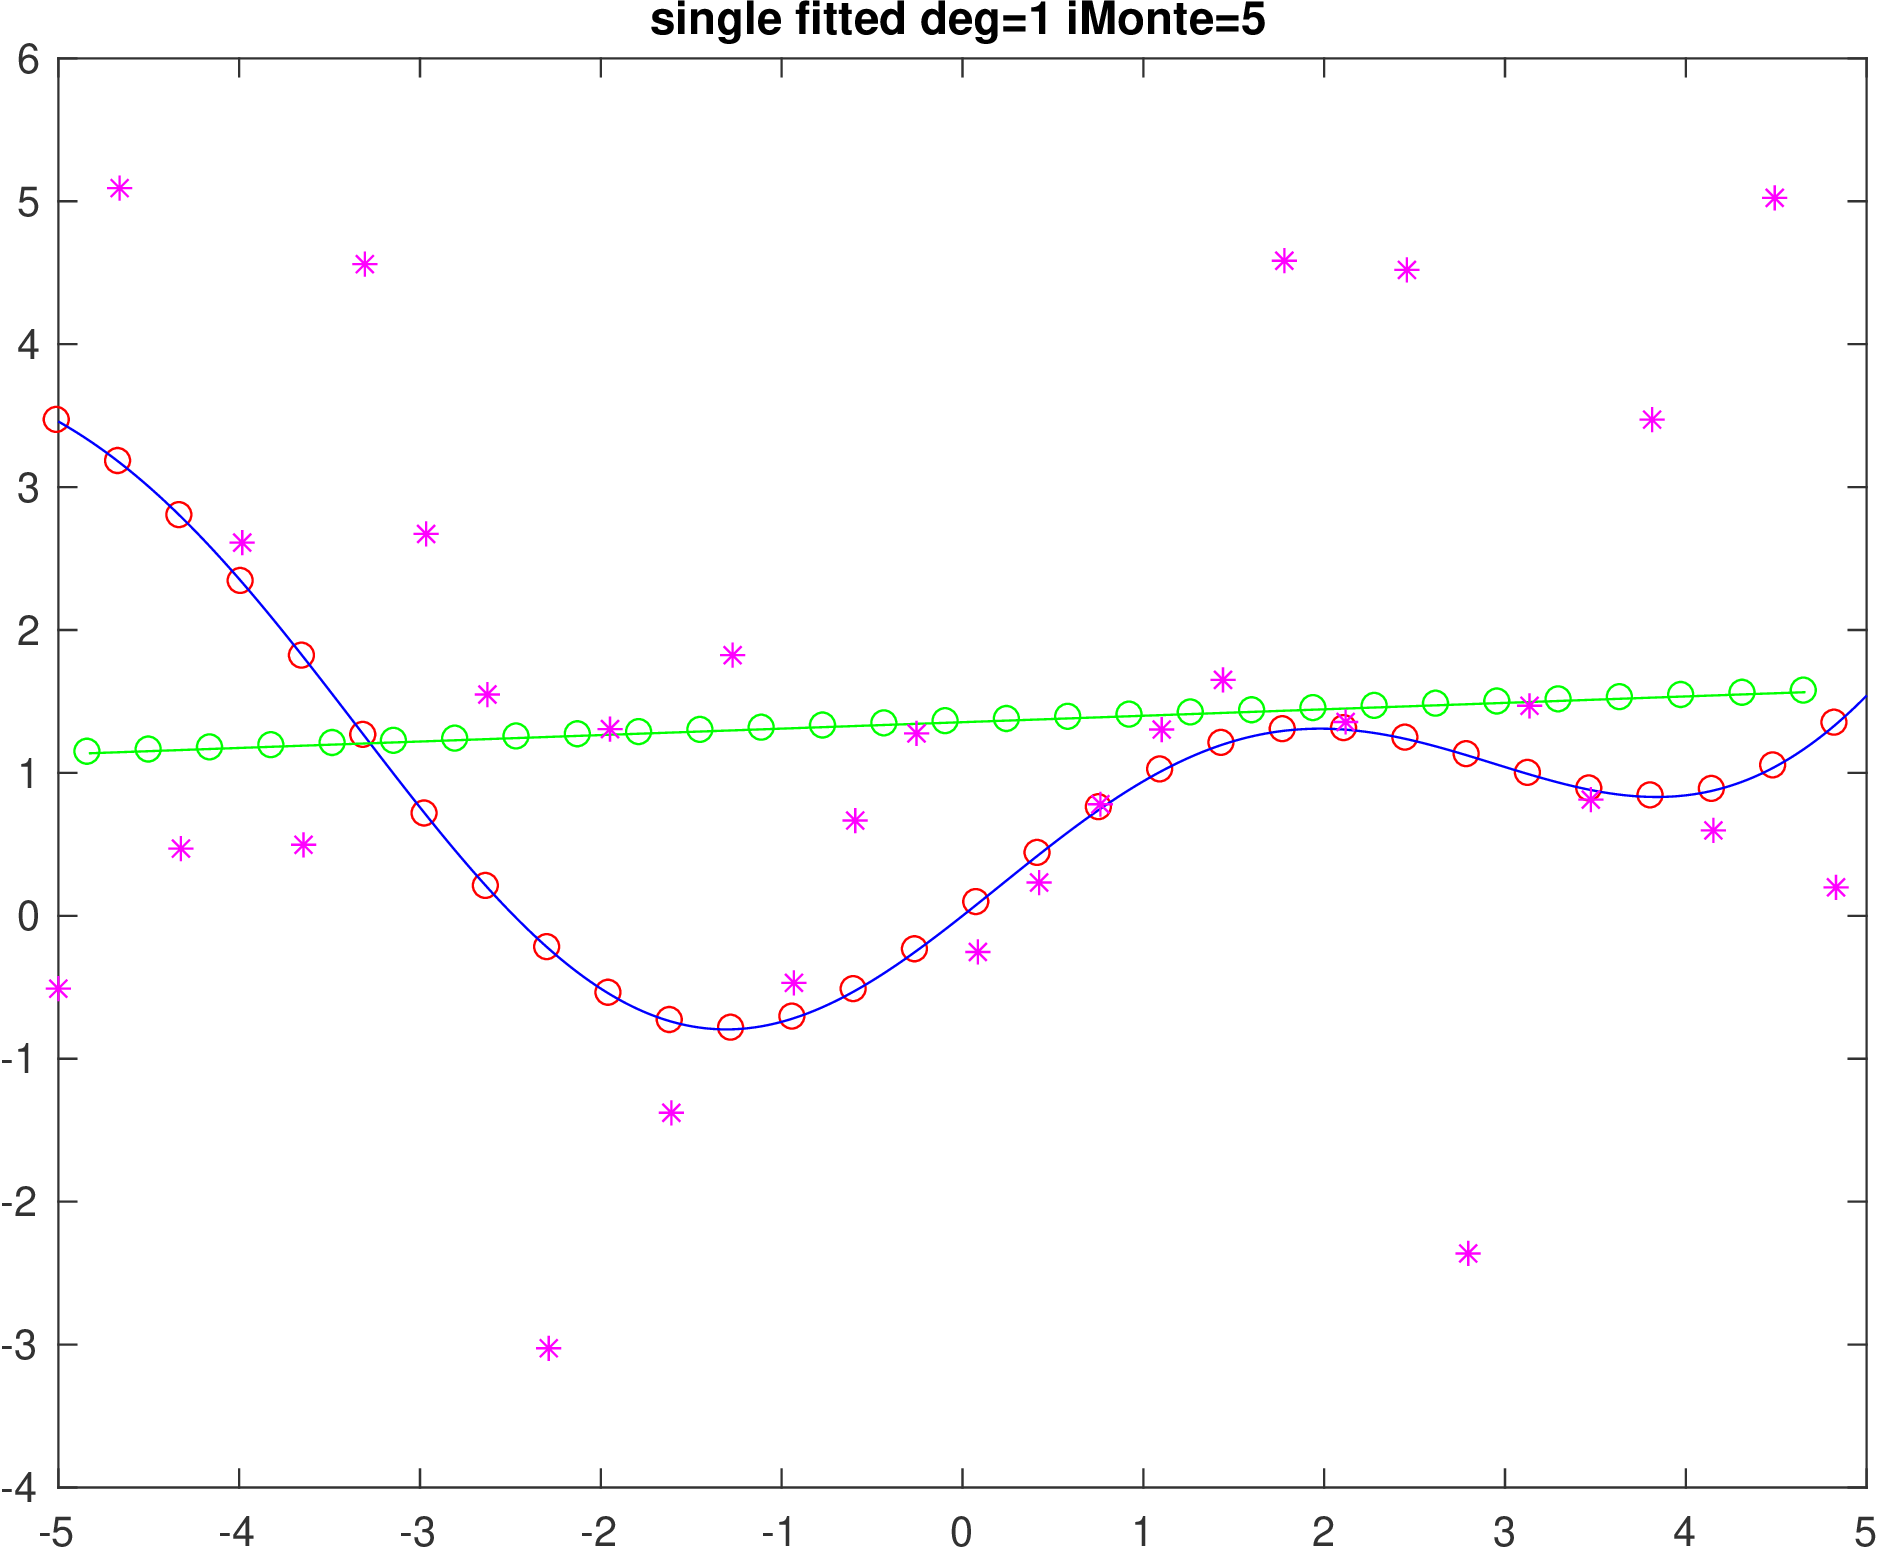
\includegraphics[scale=0.1]{single_poly_d_1_iMonte_5.png}
\end{figure}


\begin{figure}[h!]
\centering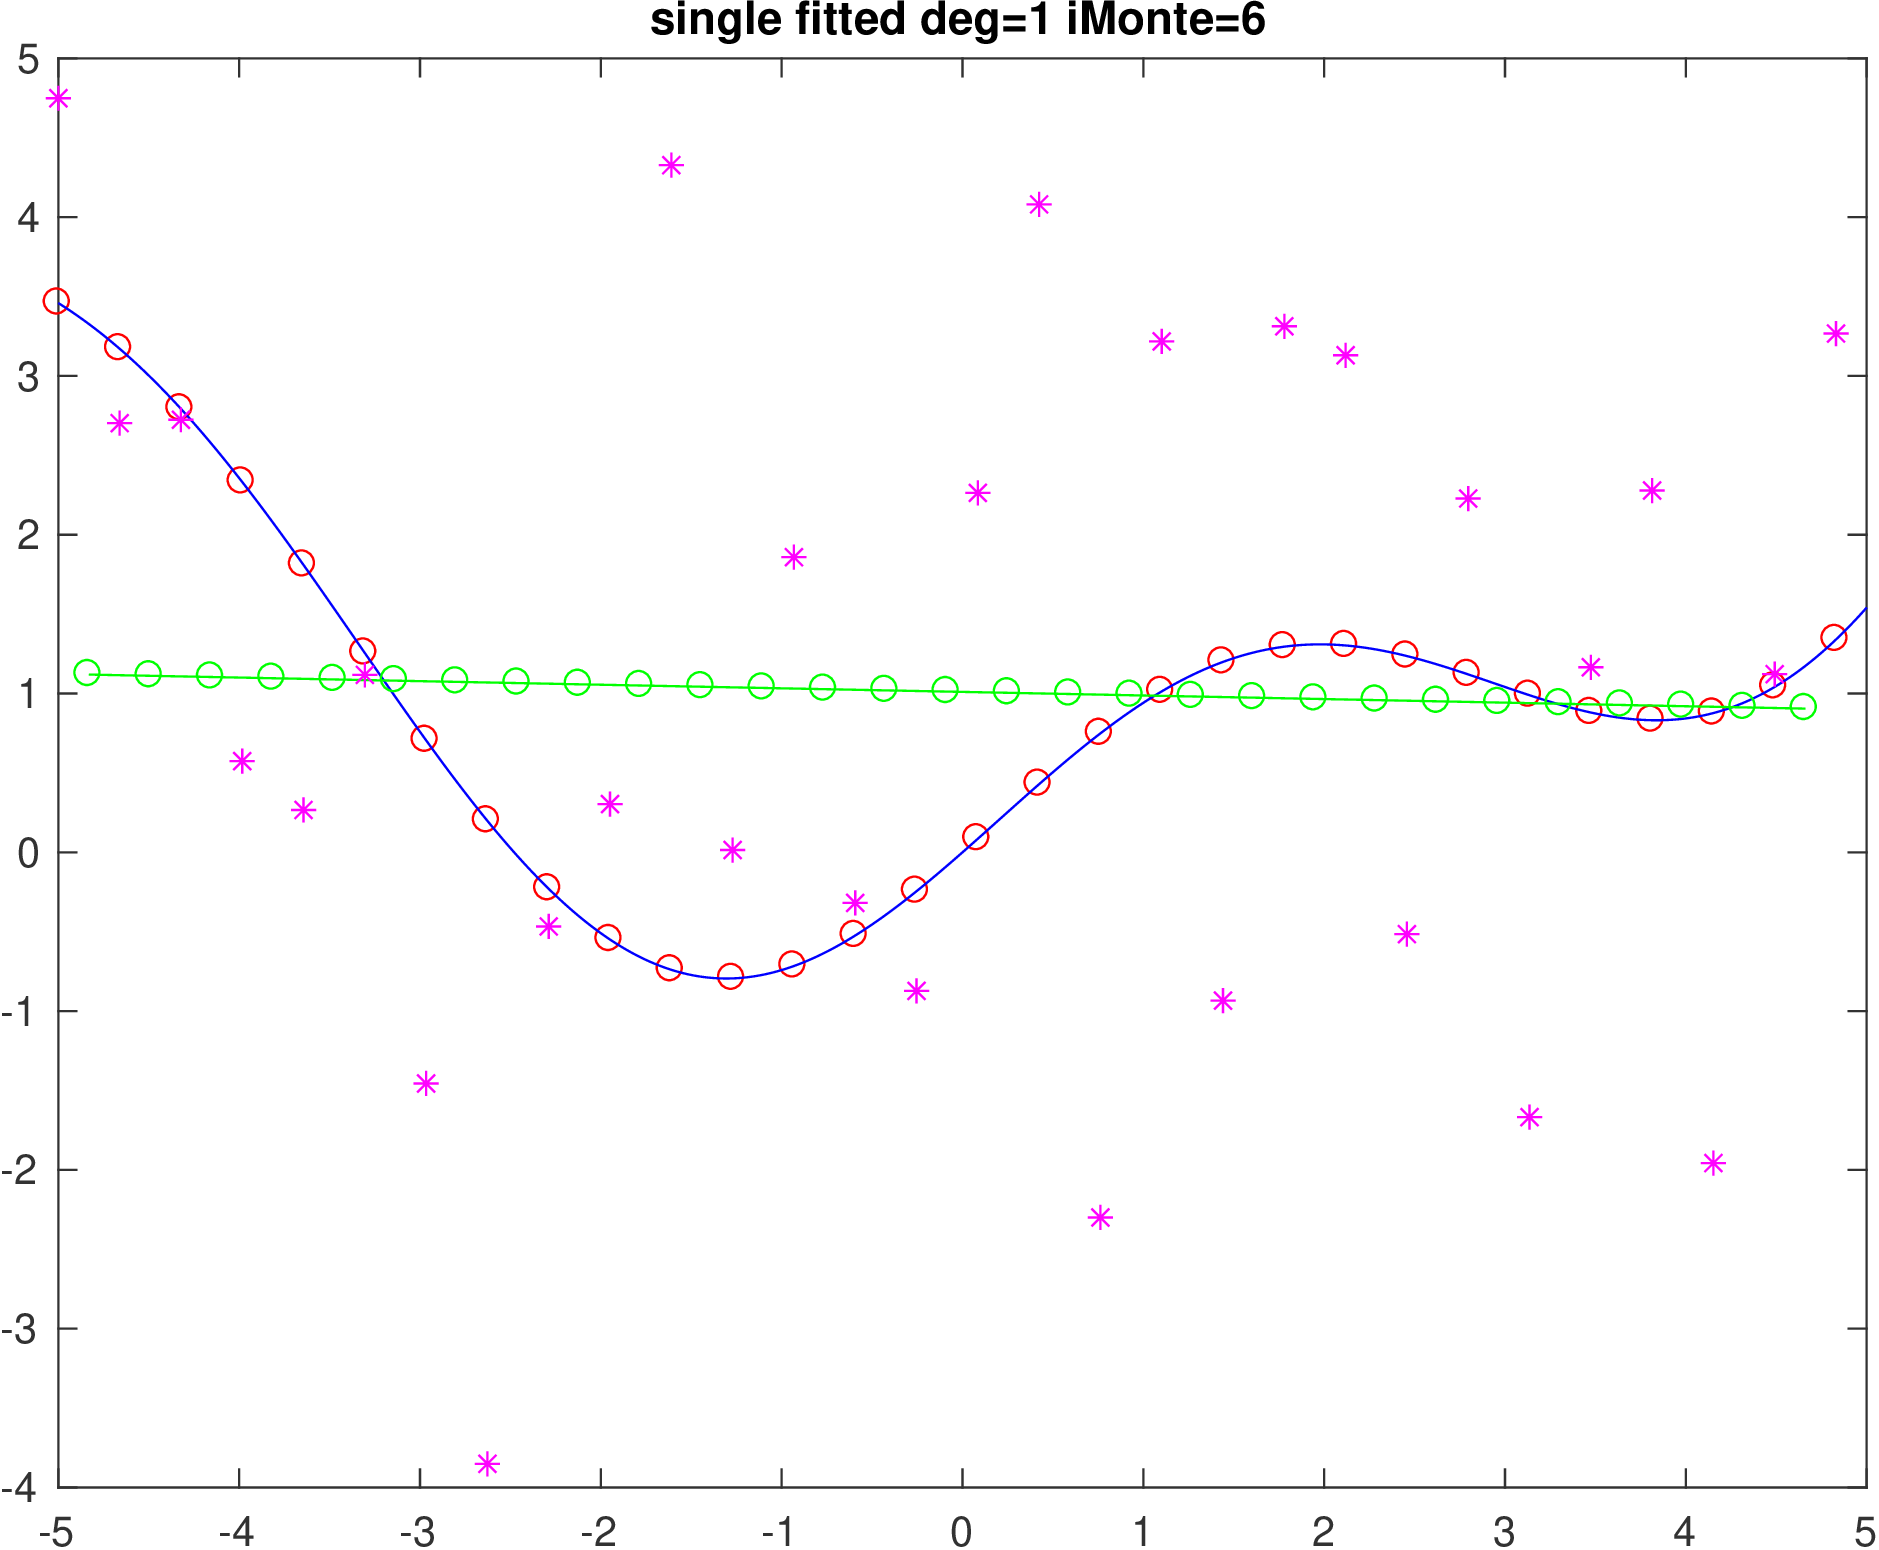
\includegraphics[scale=0.1]{single_poly_d_1_iMonte_6.png}
\end{figure}

\begin{figure}[h!]
\centering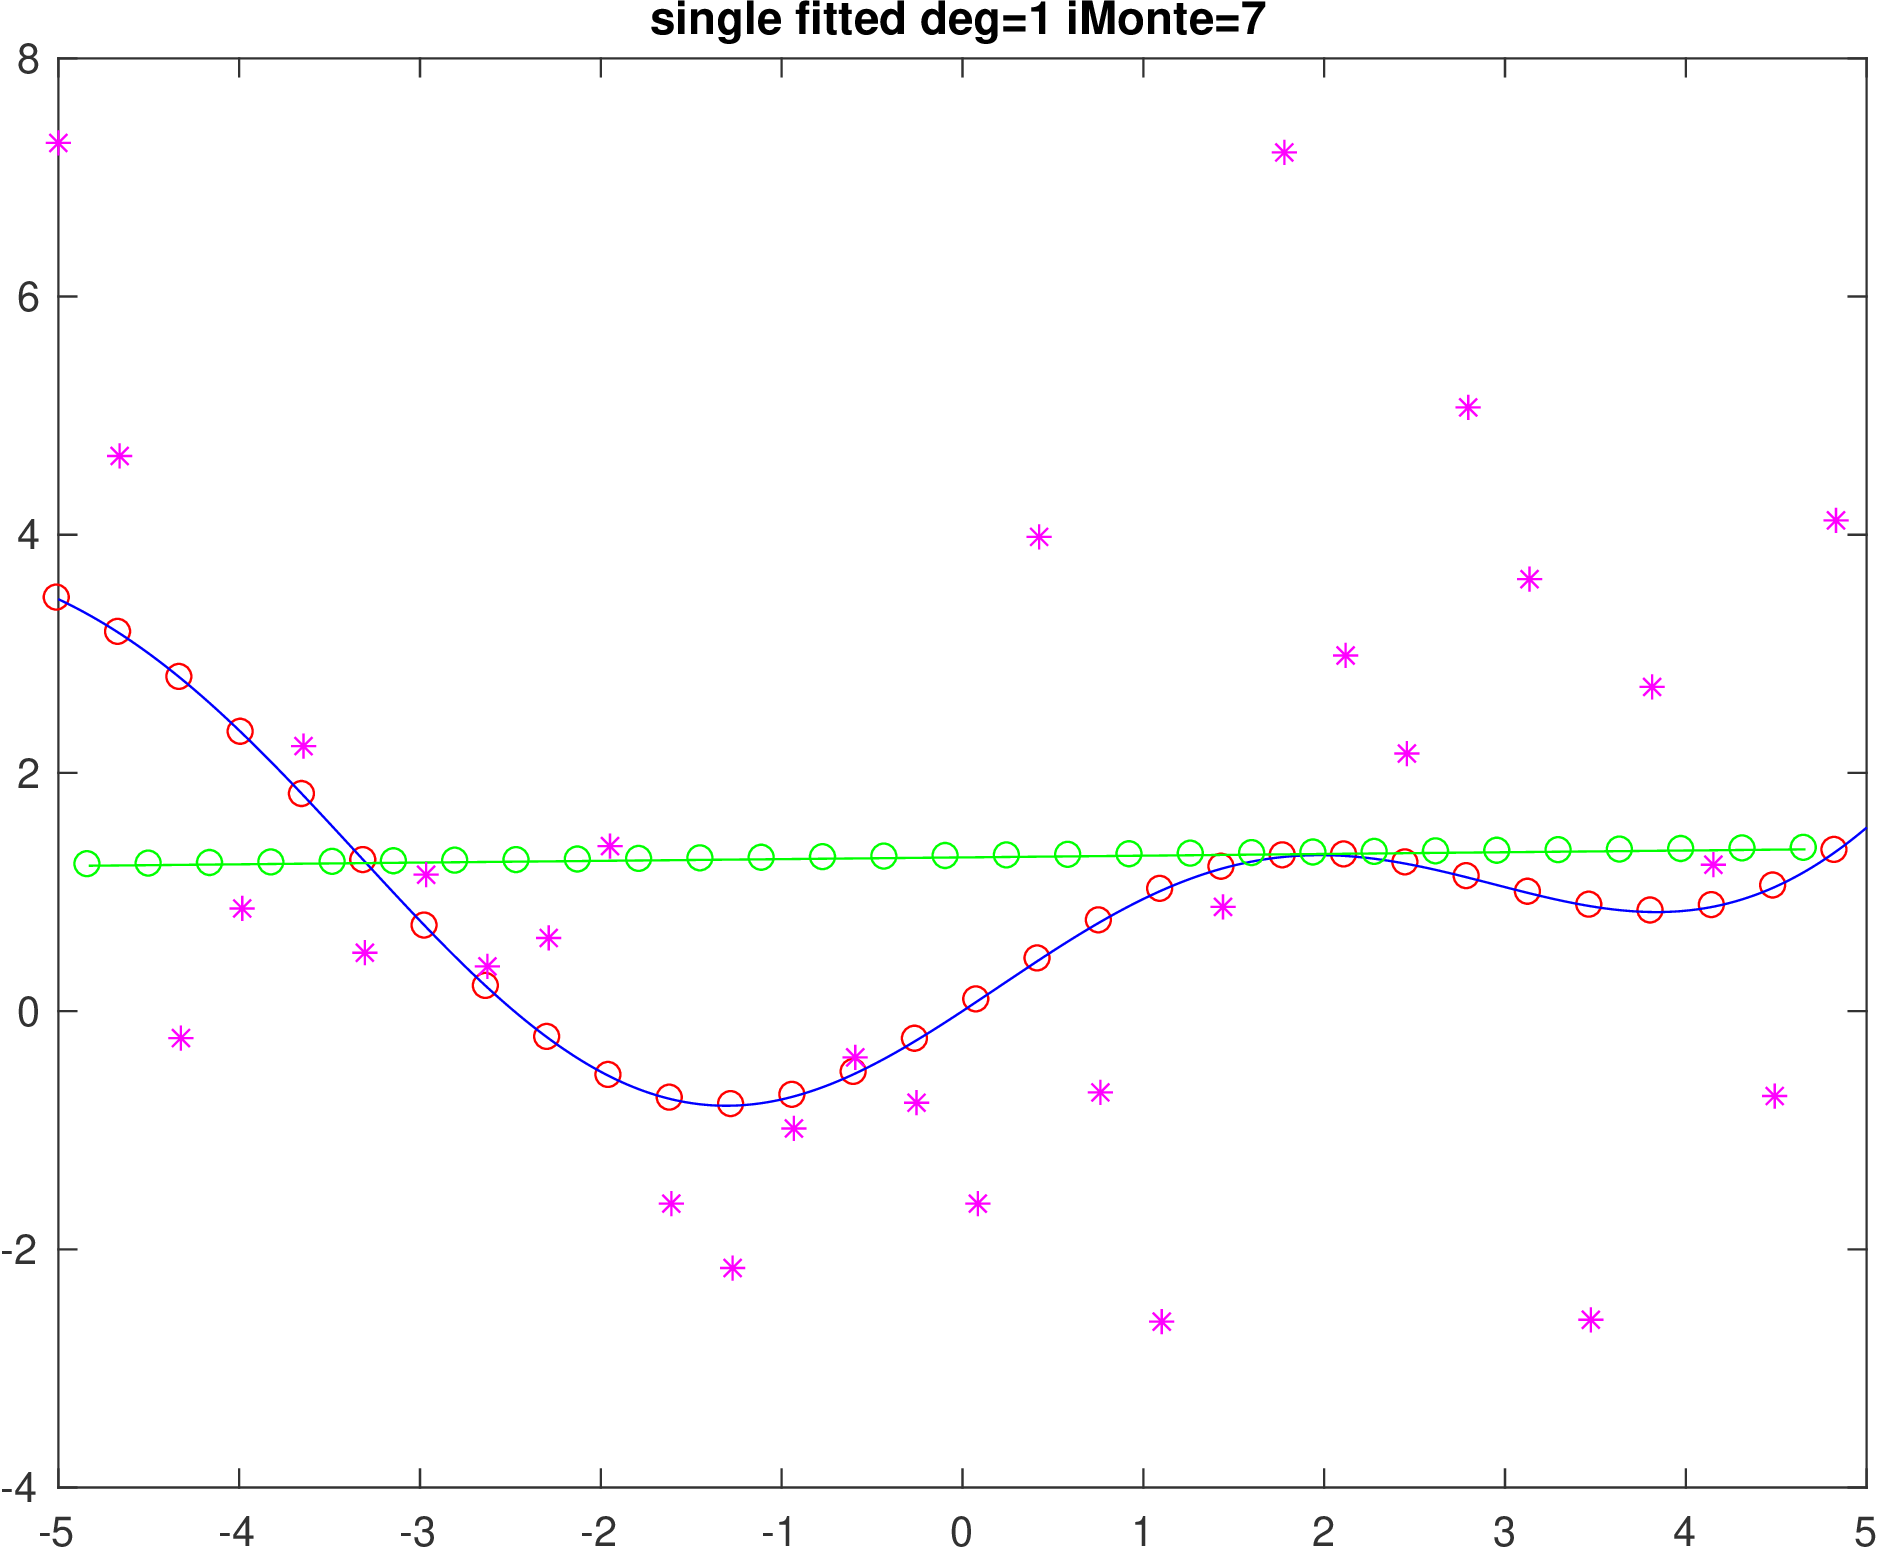
\includegraphics[scale=0.1]{single_poly_d_1_iMonte_7.png}
\end{figure}


\begin{figure}[h!]
\centering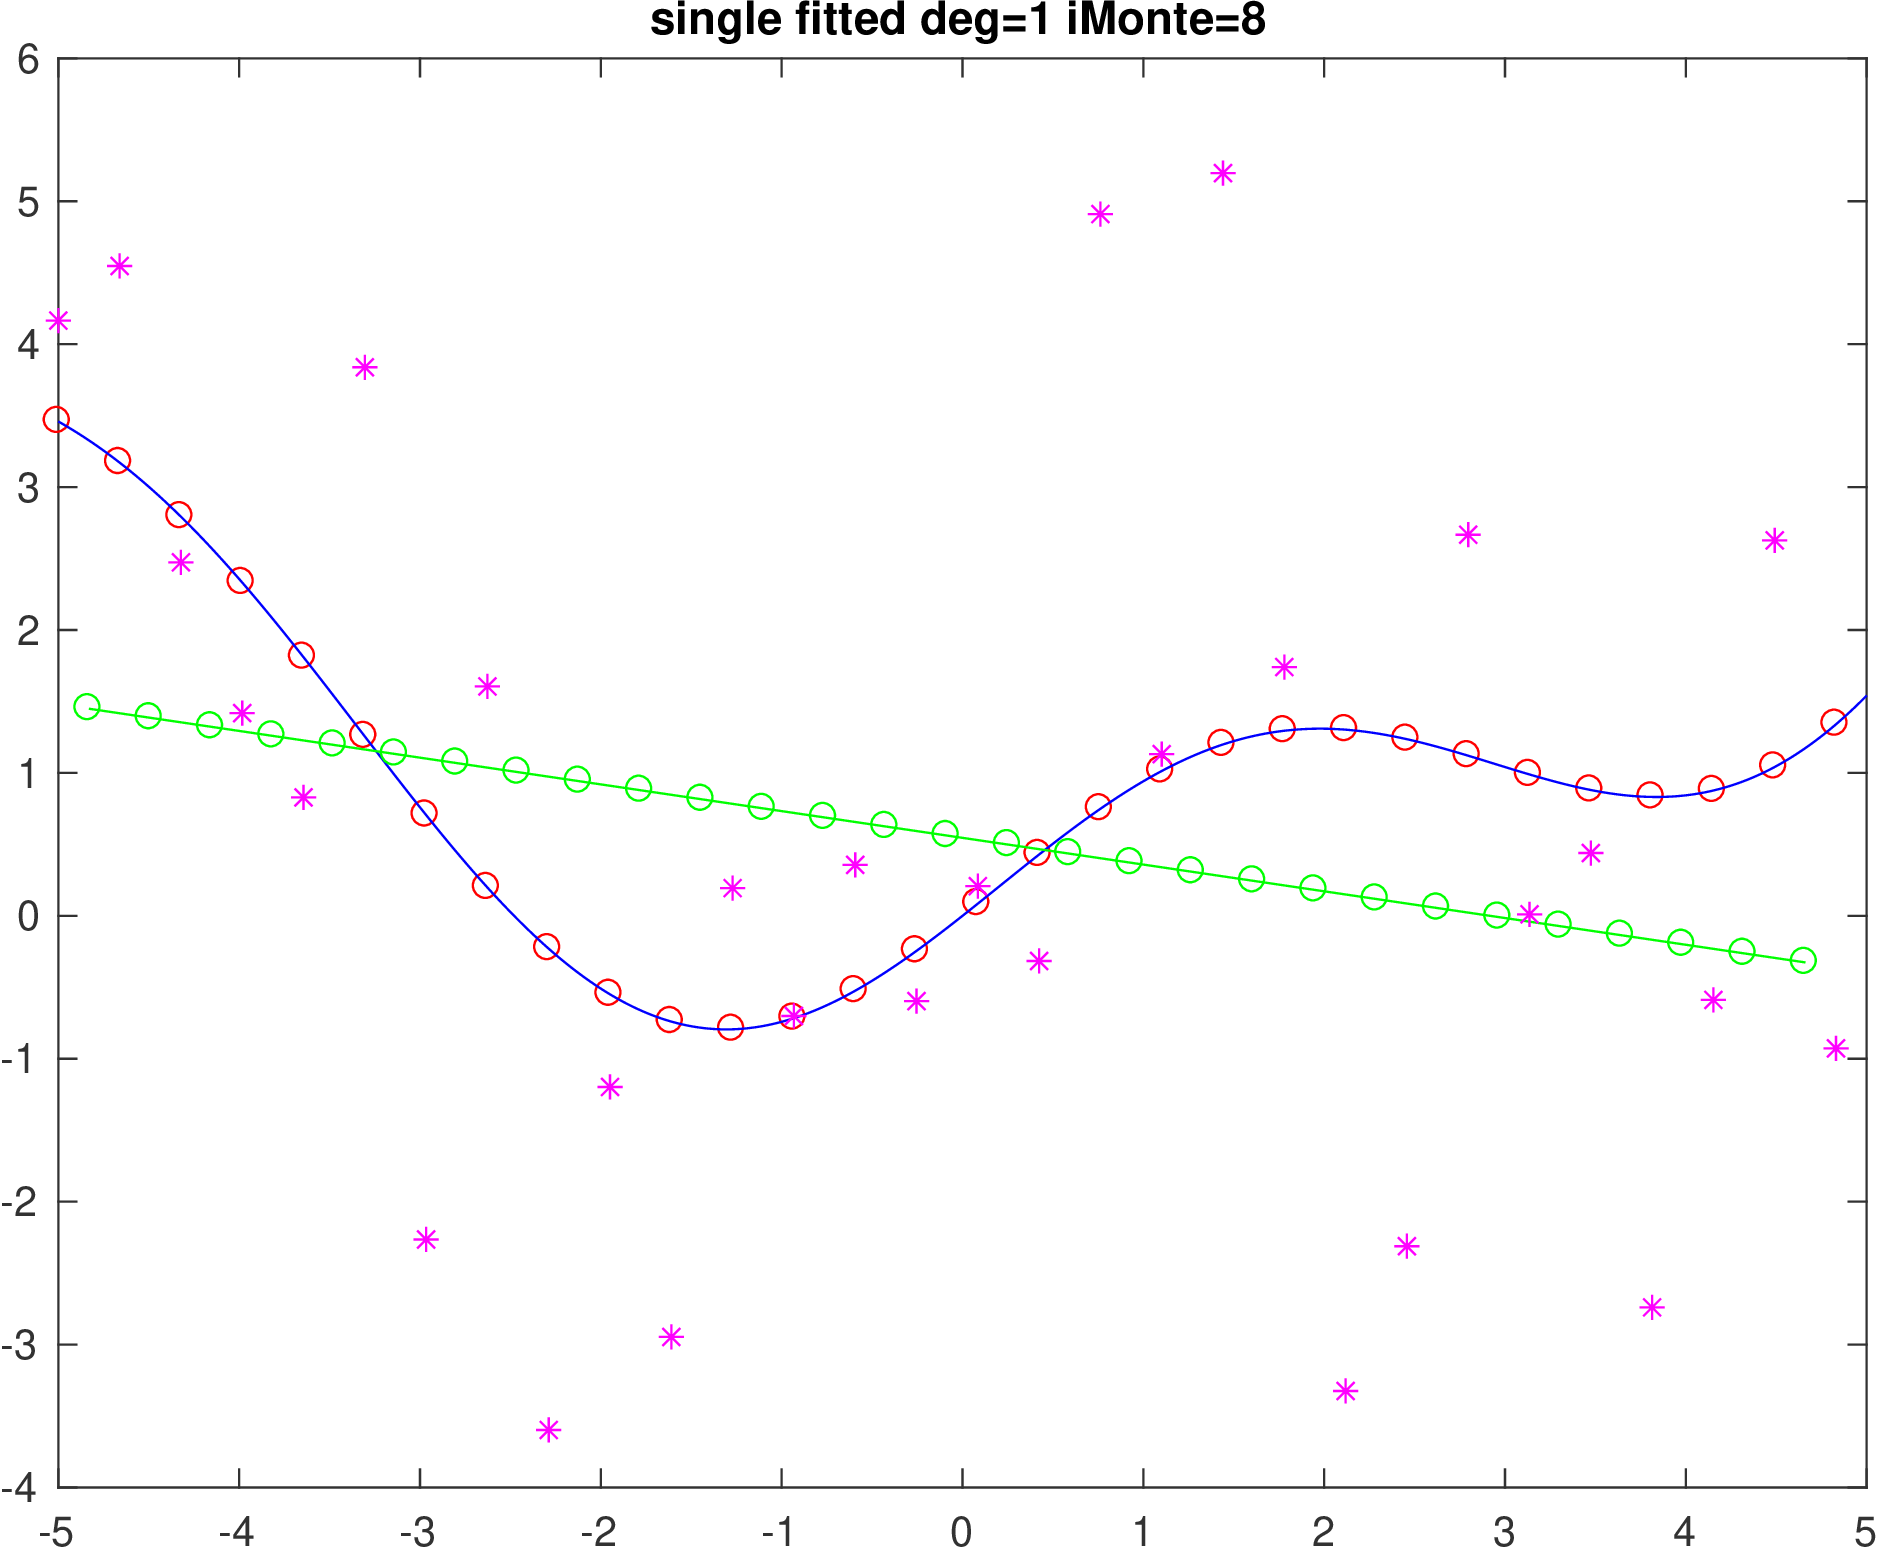
\includegraphics[scale=0.1]{single_poly_d_1_iMonte_8.png}
\end{figure}


\begin{figure}[h!]
\centering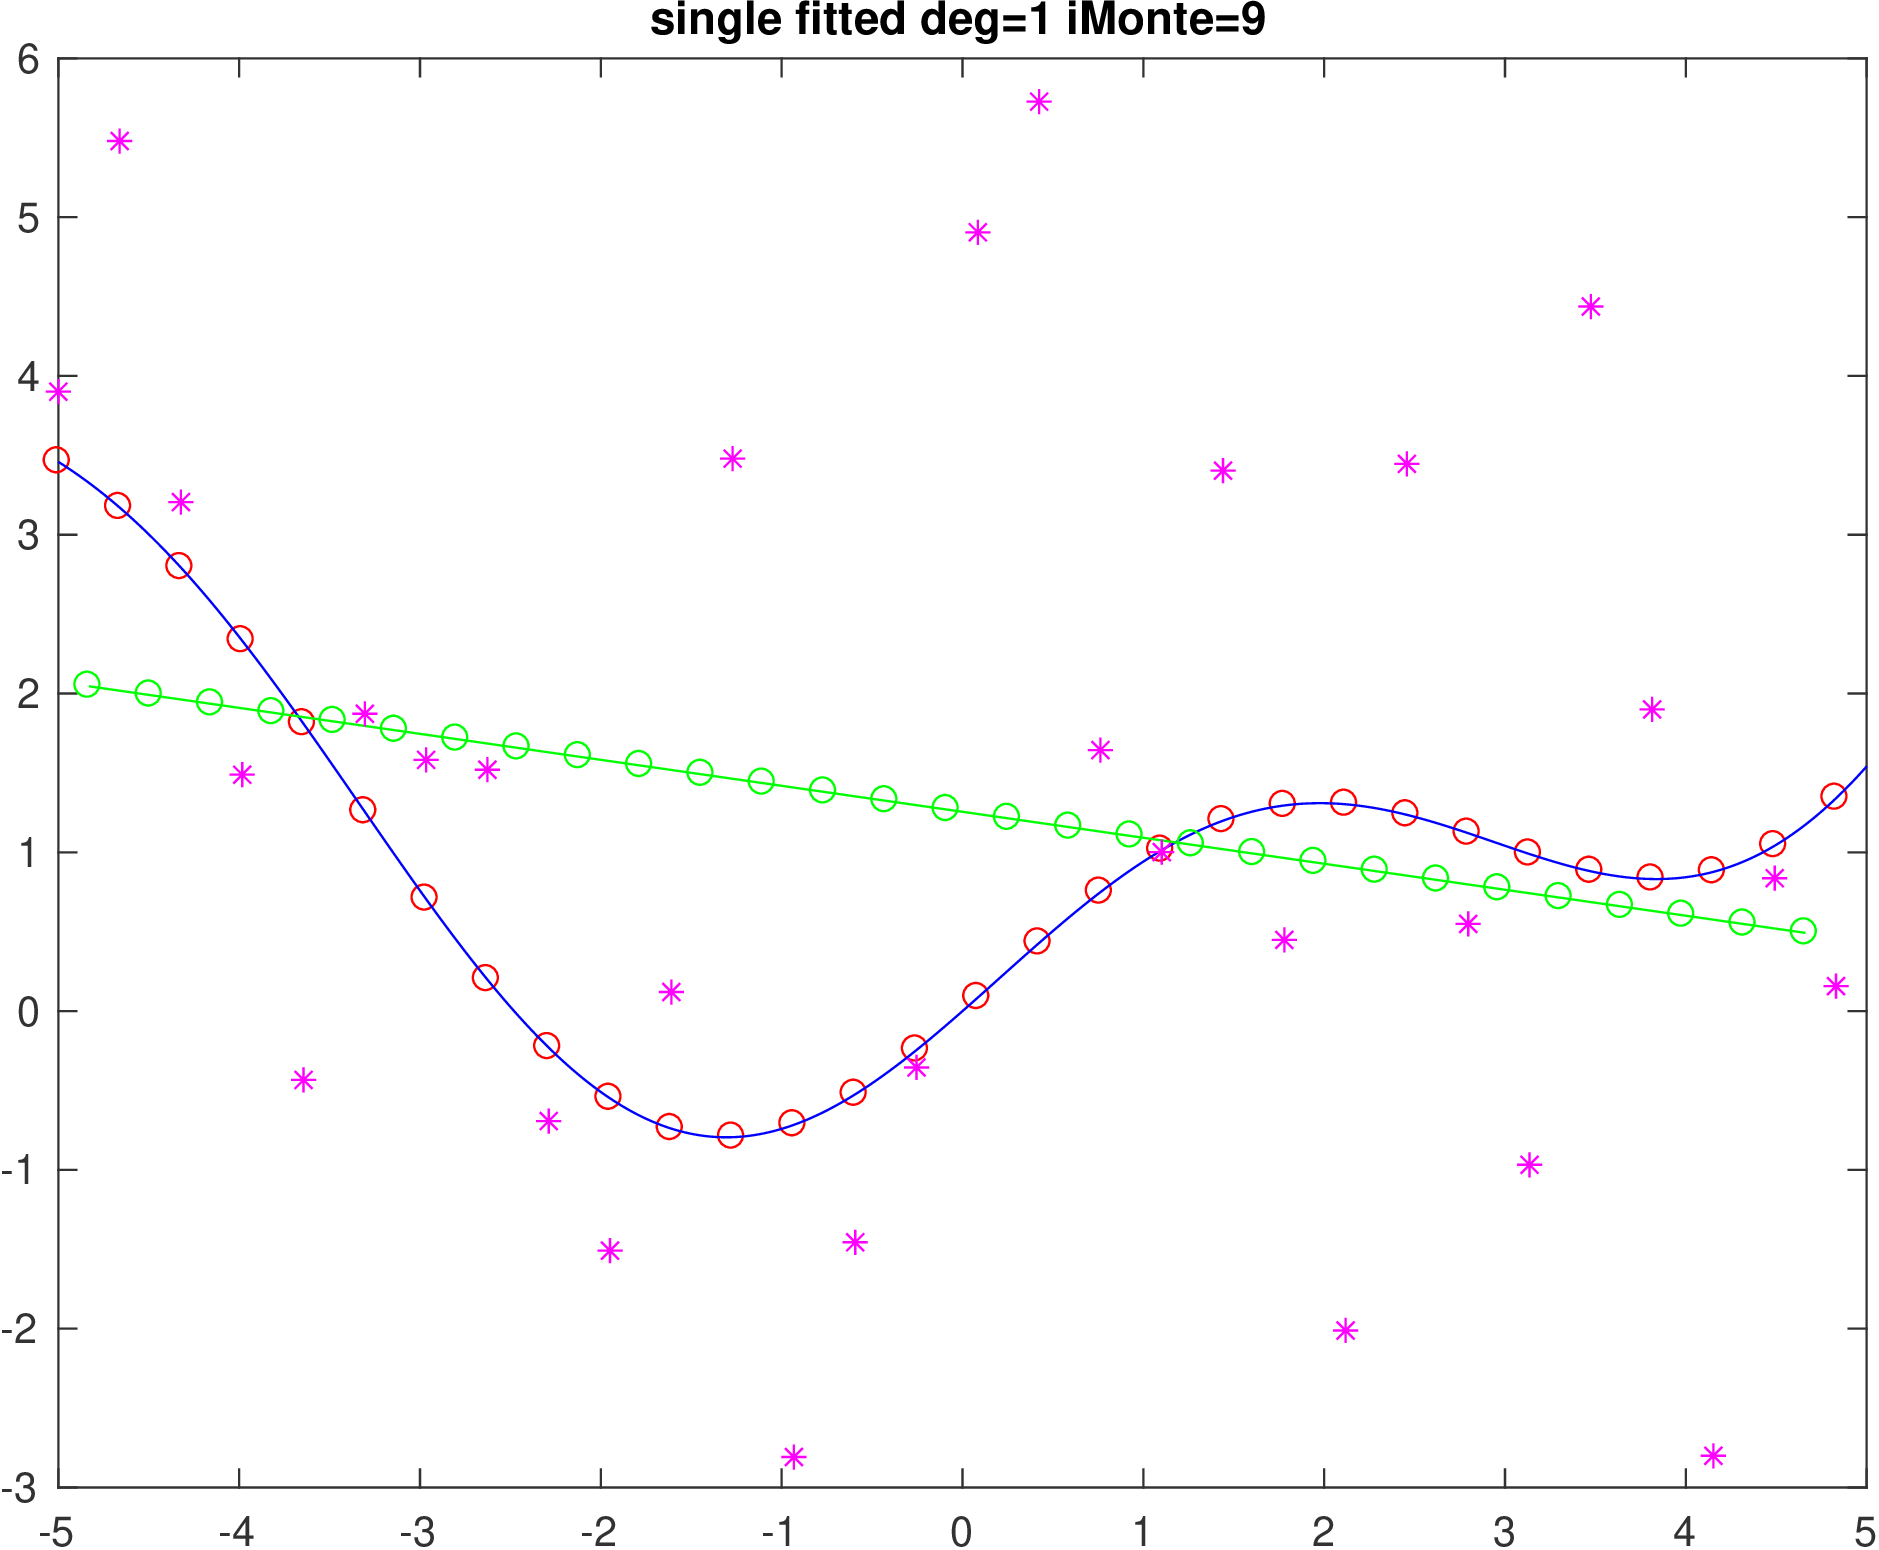
\includegraphics[scale=0.1]{single_poly_d_1_iMonte_9.png}
\end{figure}


\begin{figure}[h!]
\centering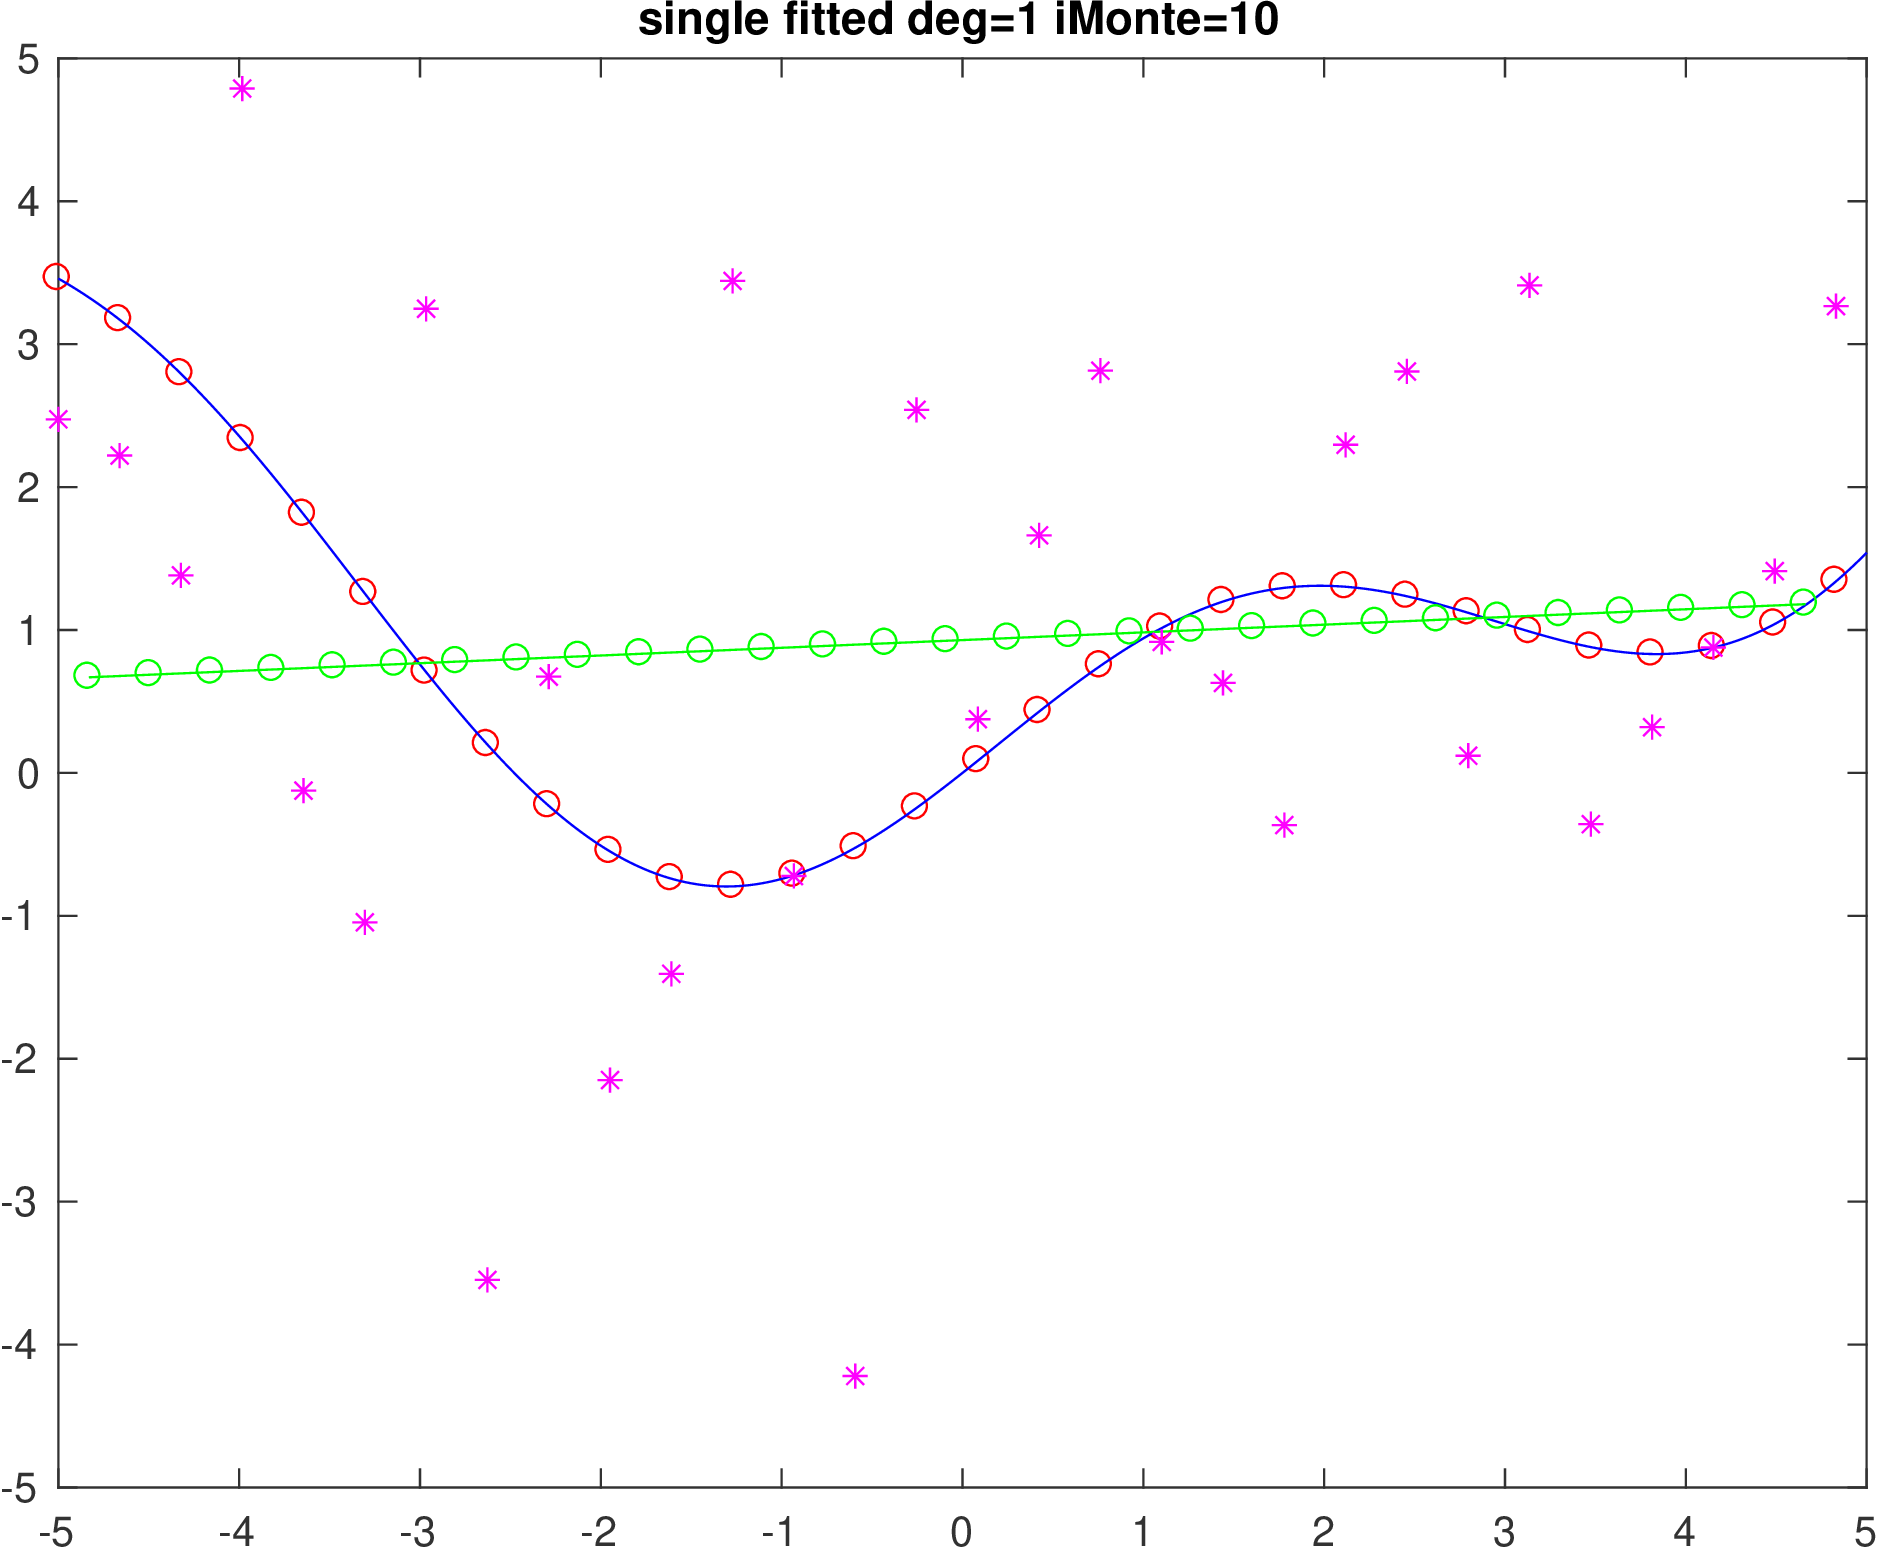
\includegraphics[scale=0.1]{single_poly_d_1_iMonte_10.png}
\end{figure}


\begin{figure}[h!]
\centering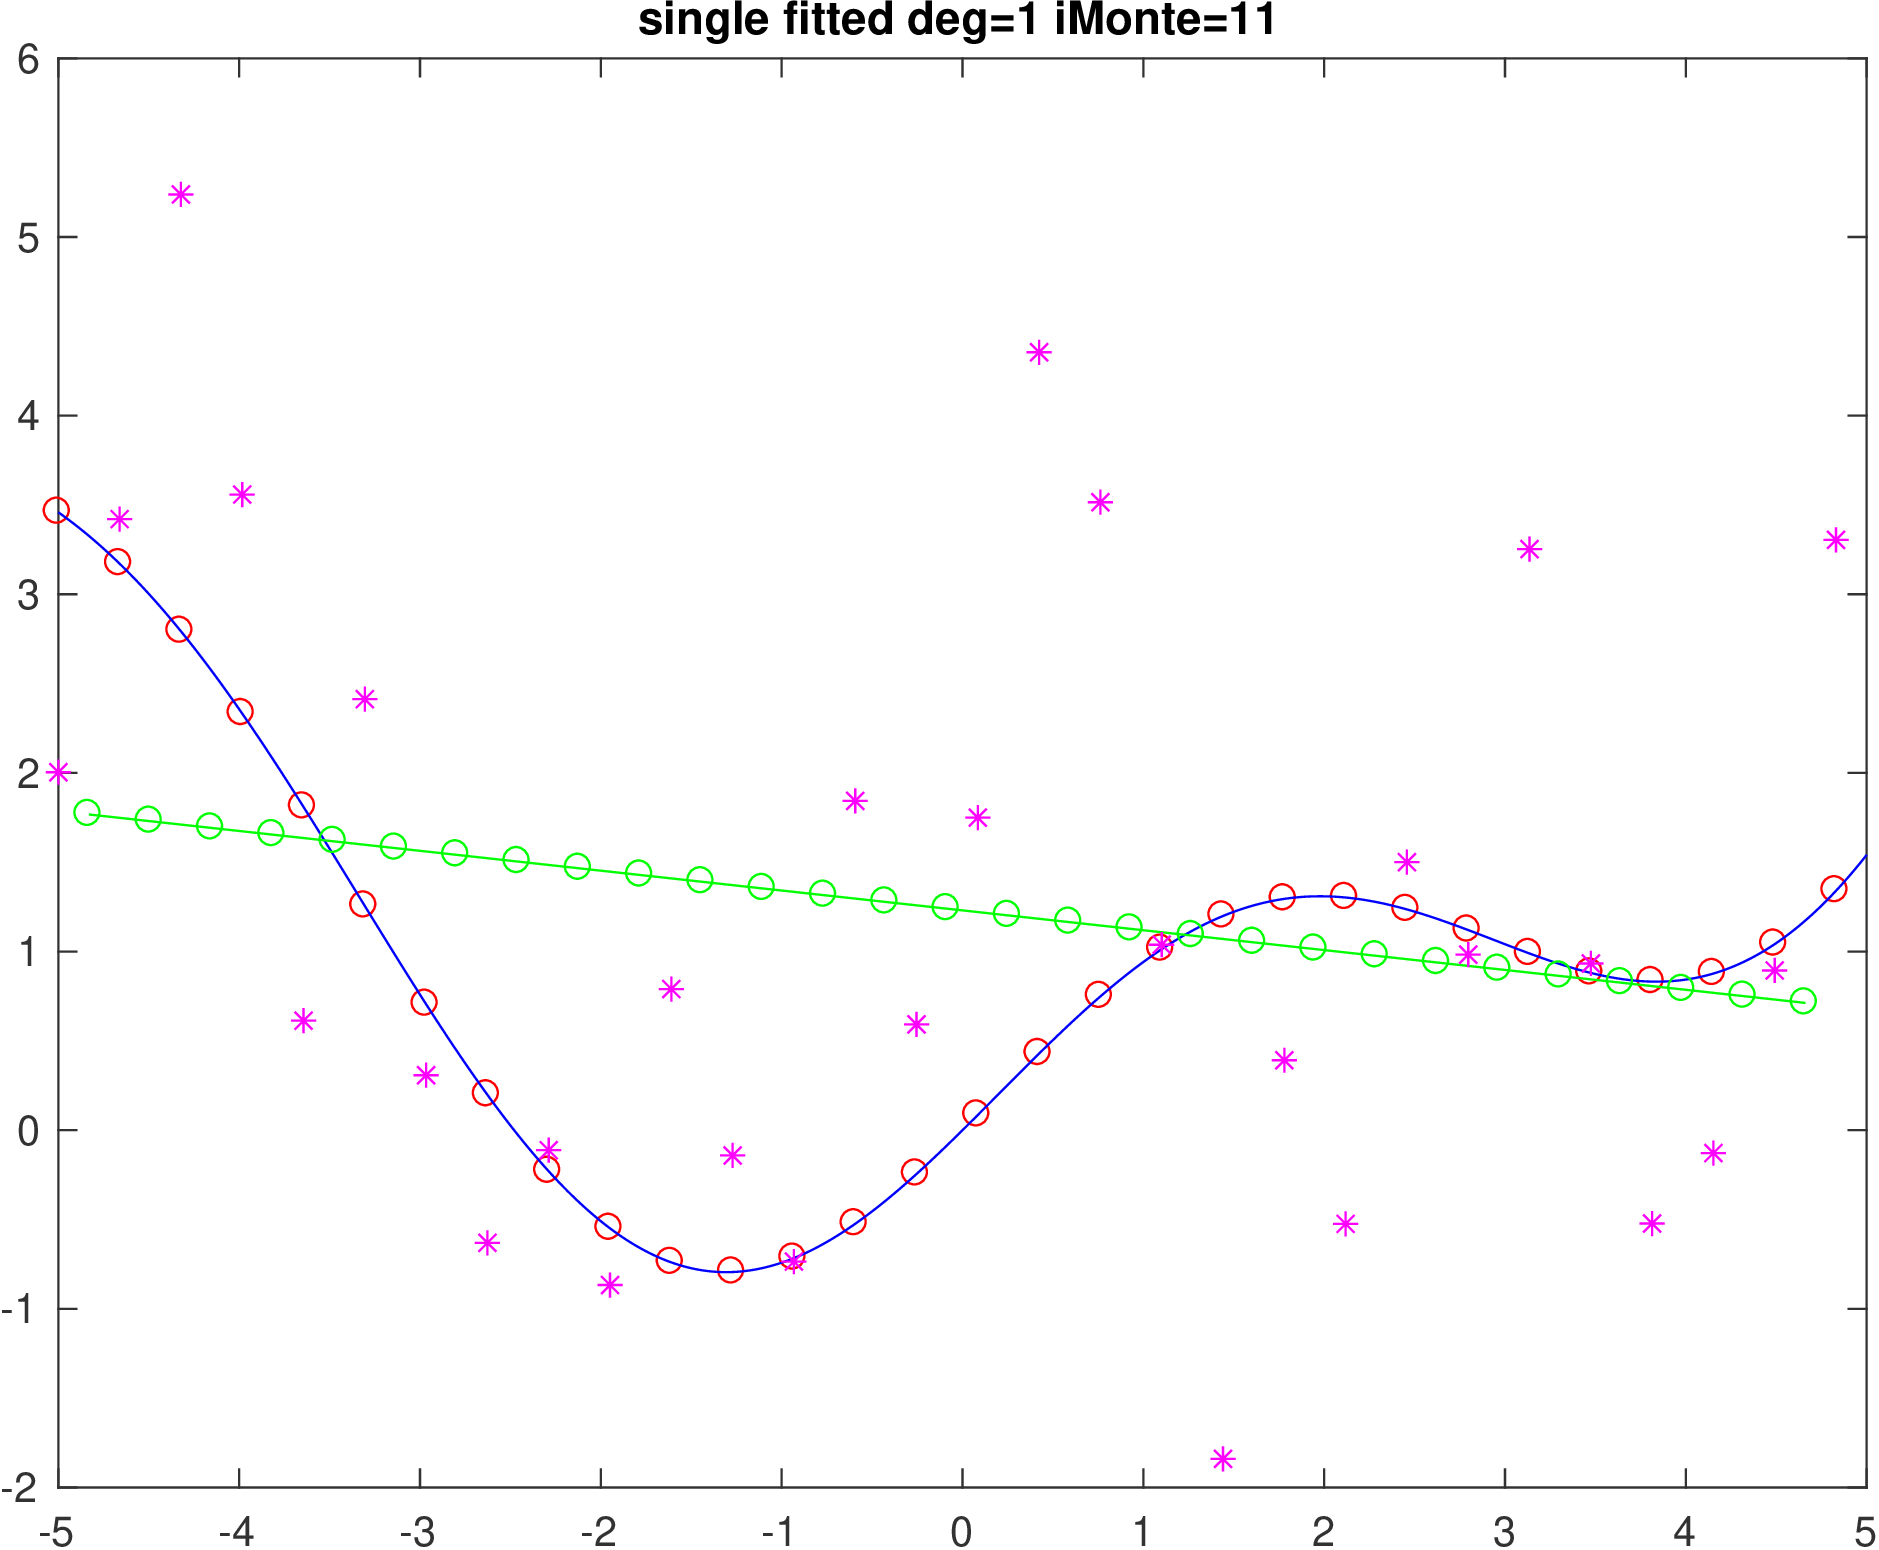
\includegraphics[scale=0.1]{single_poly_d_1_iMonte_11.png}
\end{figure}


\begin{figure}[h!]
\centering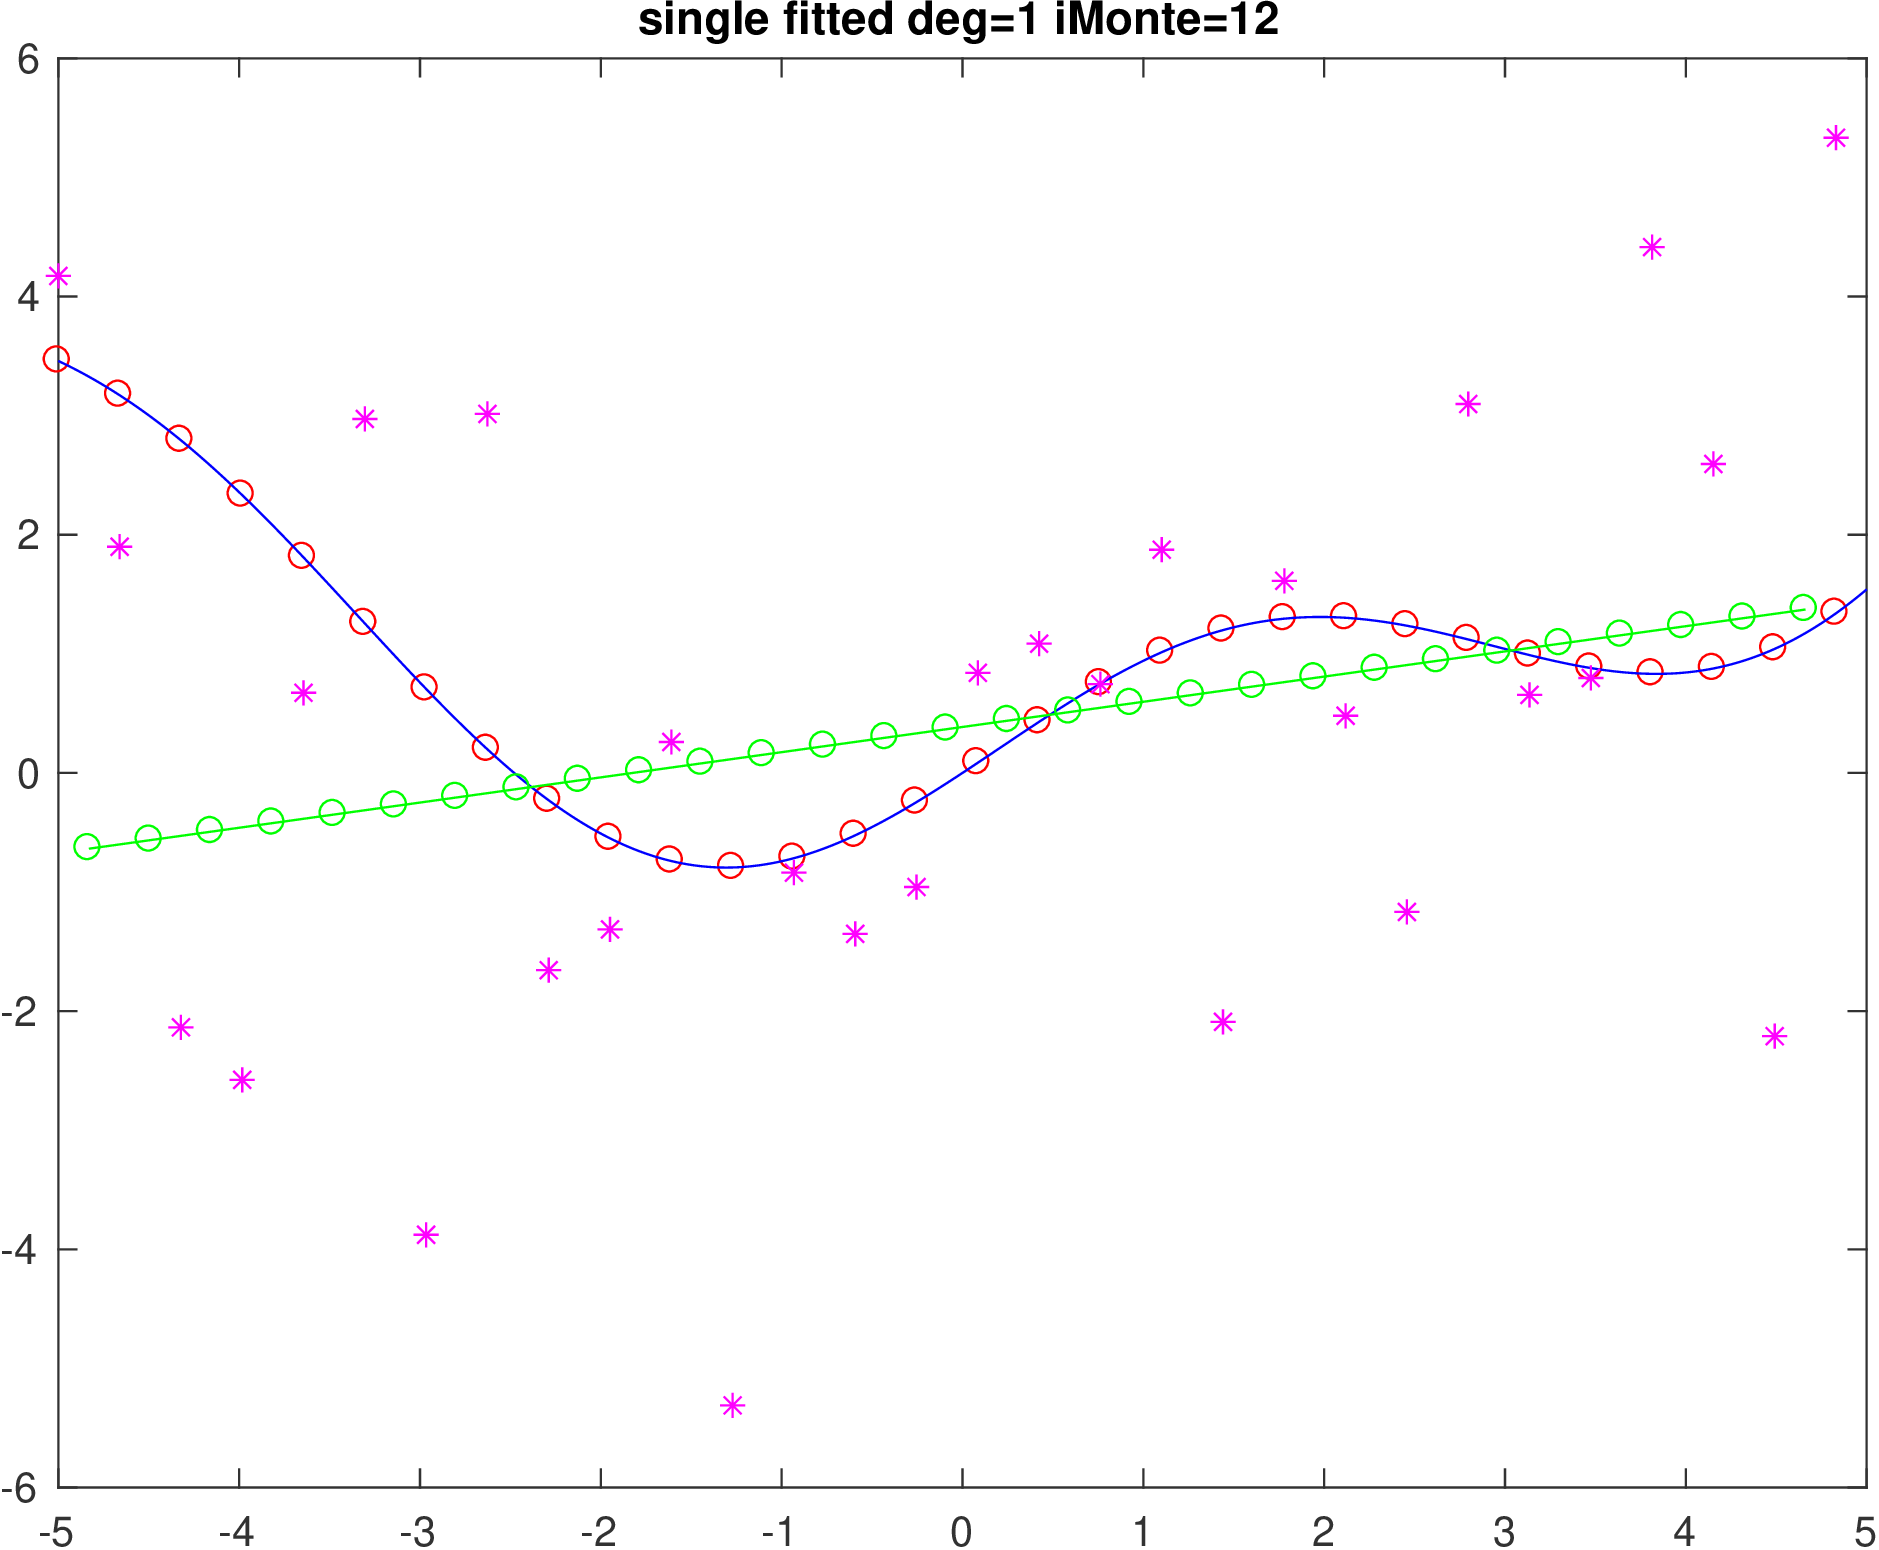
\includegraphics[scale=0.1]{single_poly_d_1_iMonte_12.png}
\end{figure}



\begin{figure}[h!]
\centering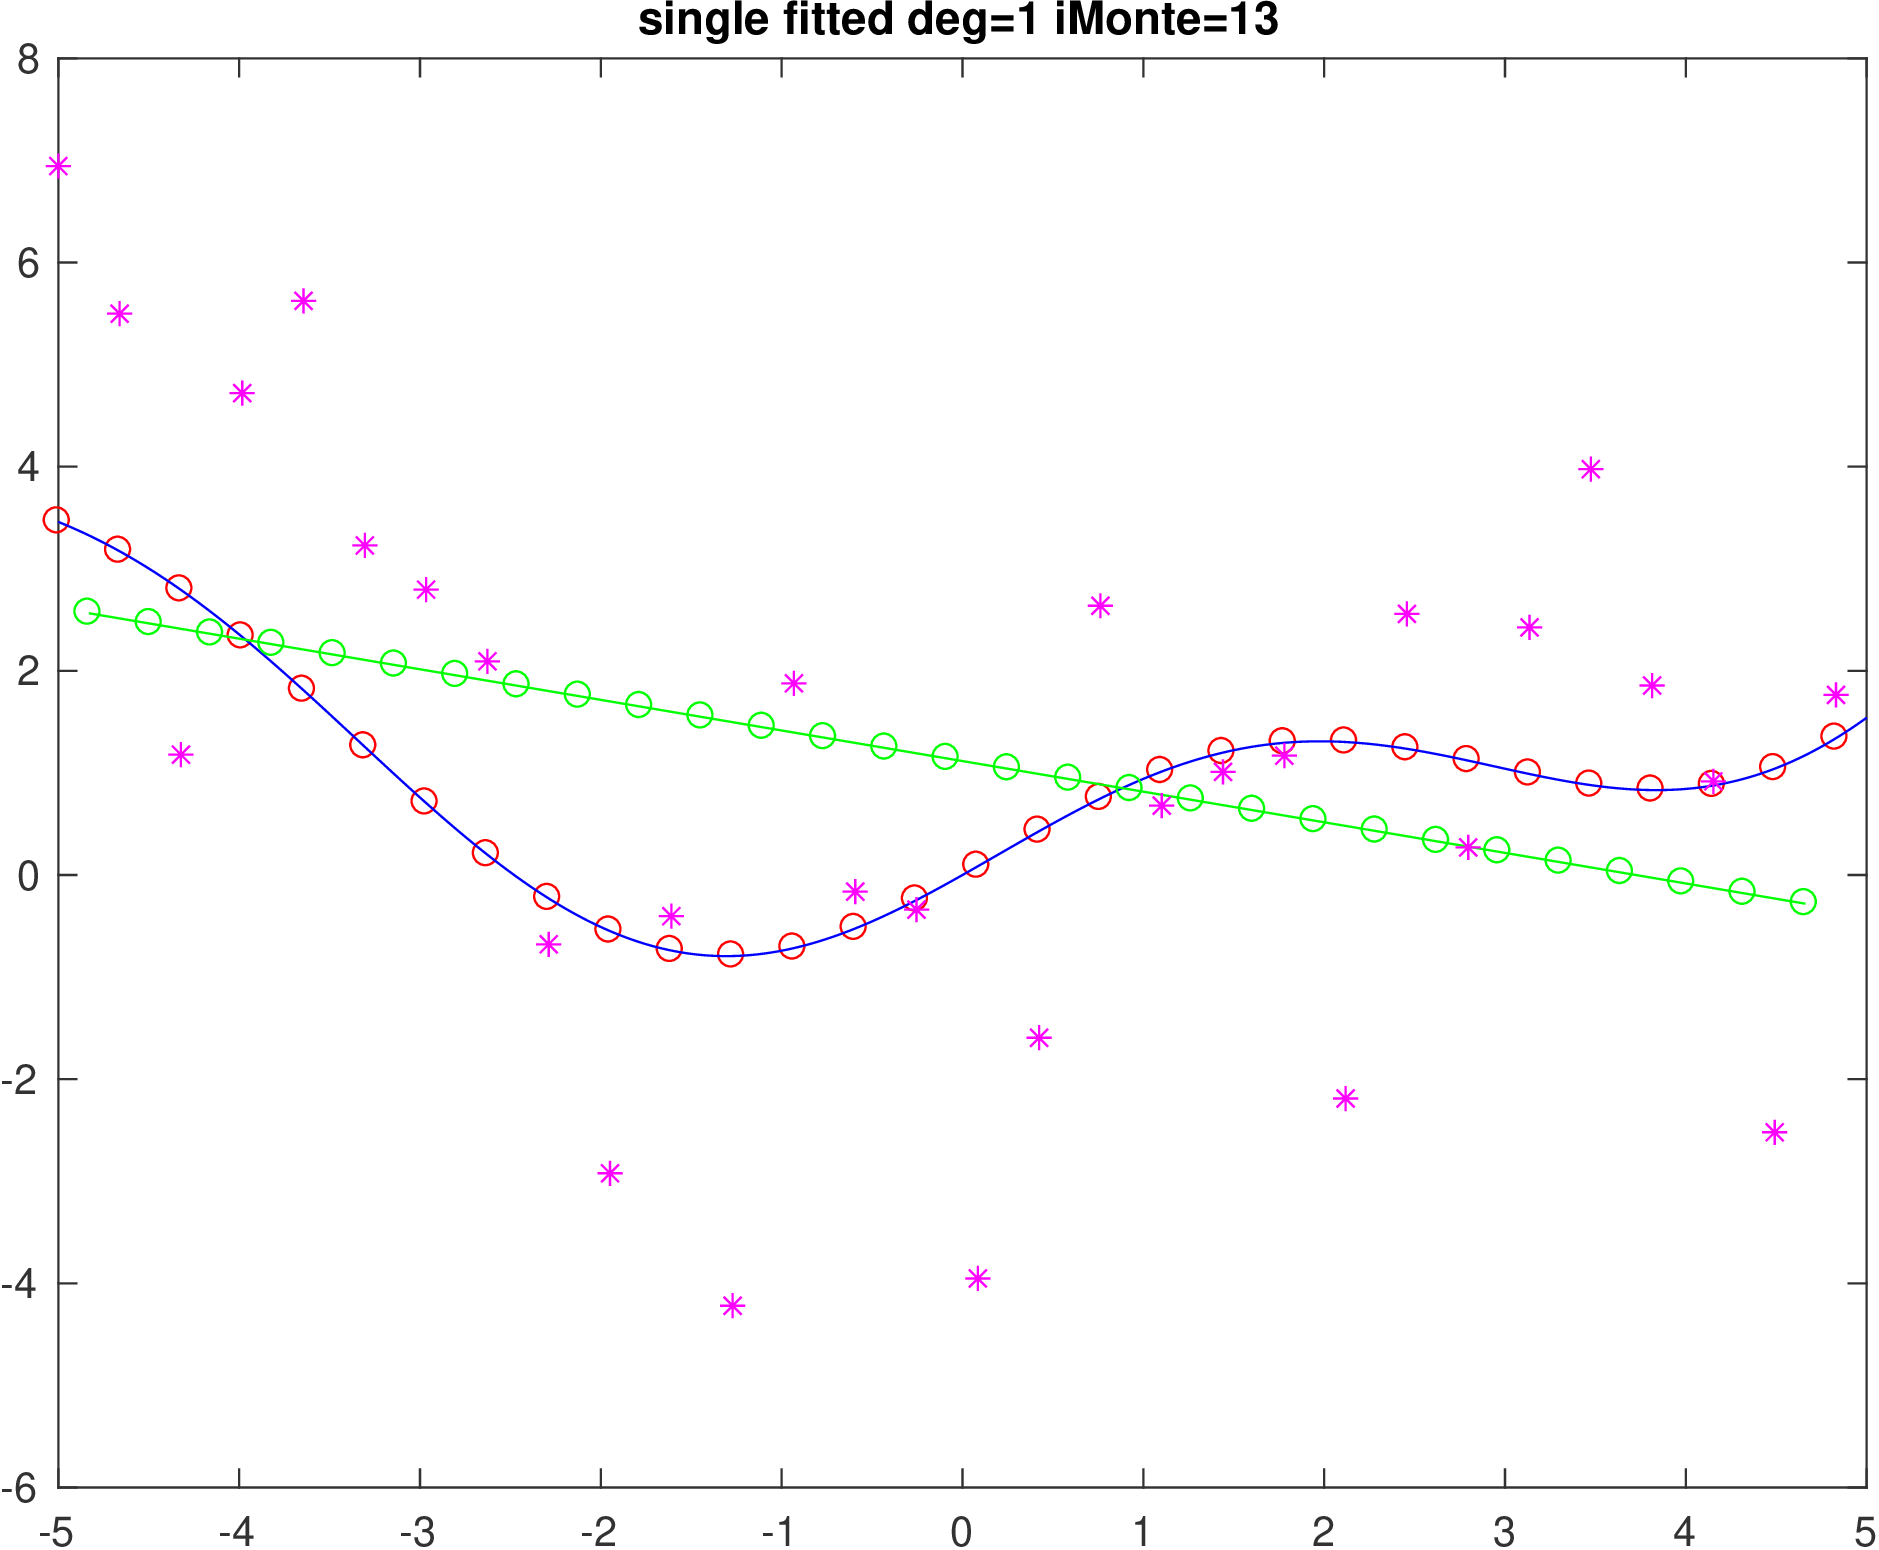
\includegraphics[scale=0.1]{single_poly_d_1_iMonte_13.png}
\end{figure}


\begin{figure}[h!]
\centering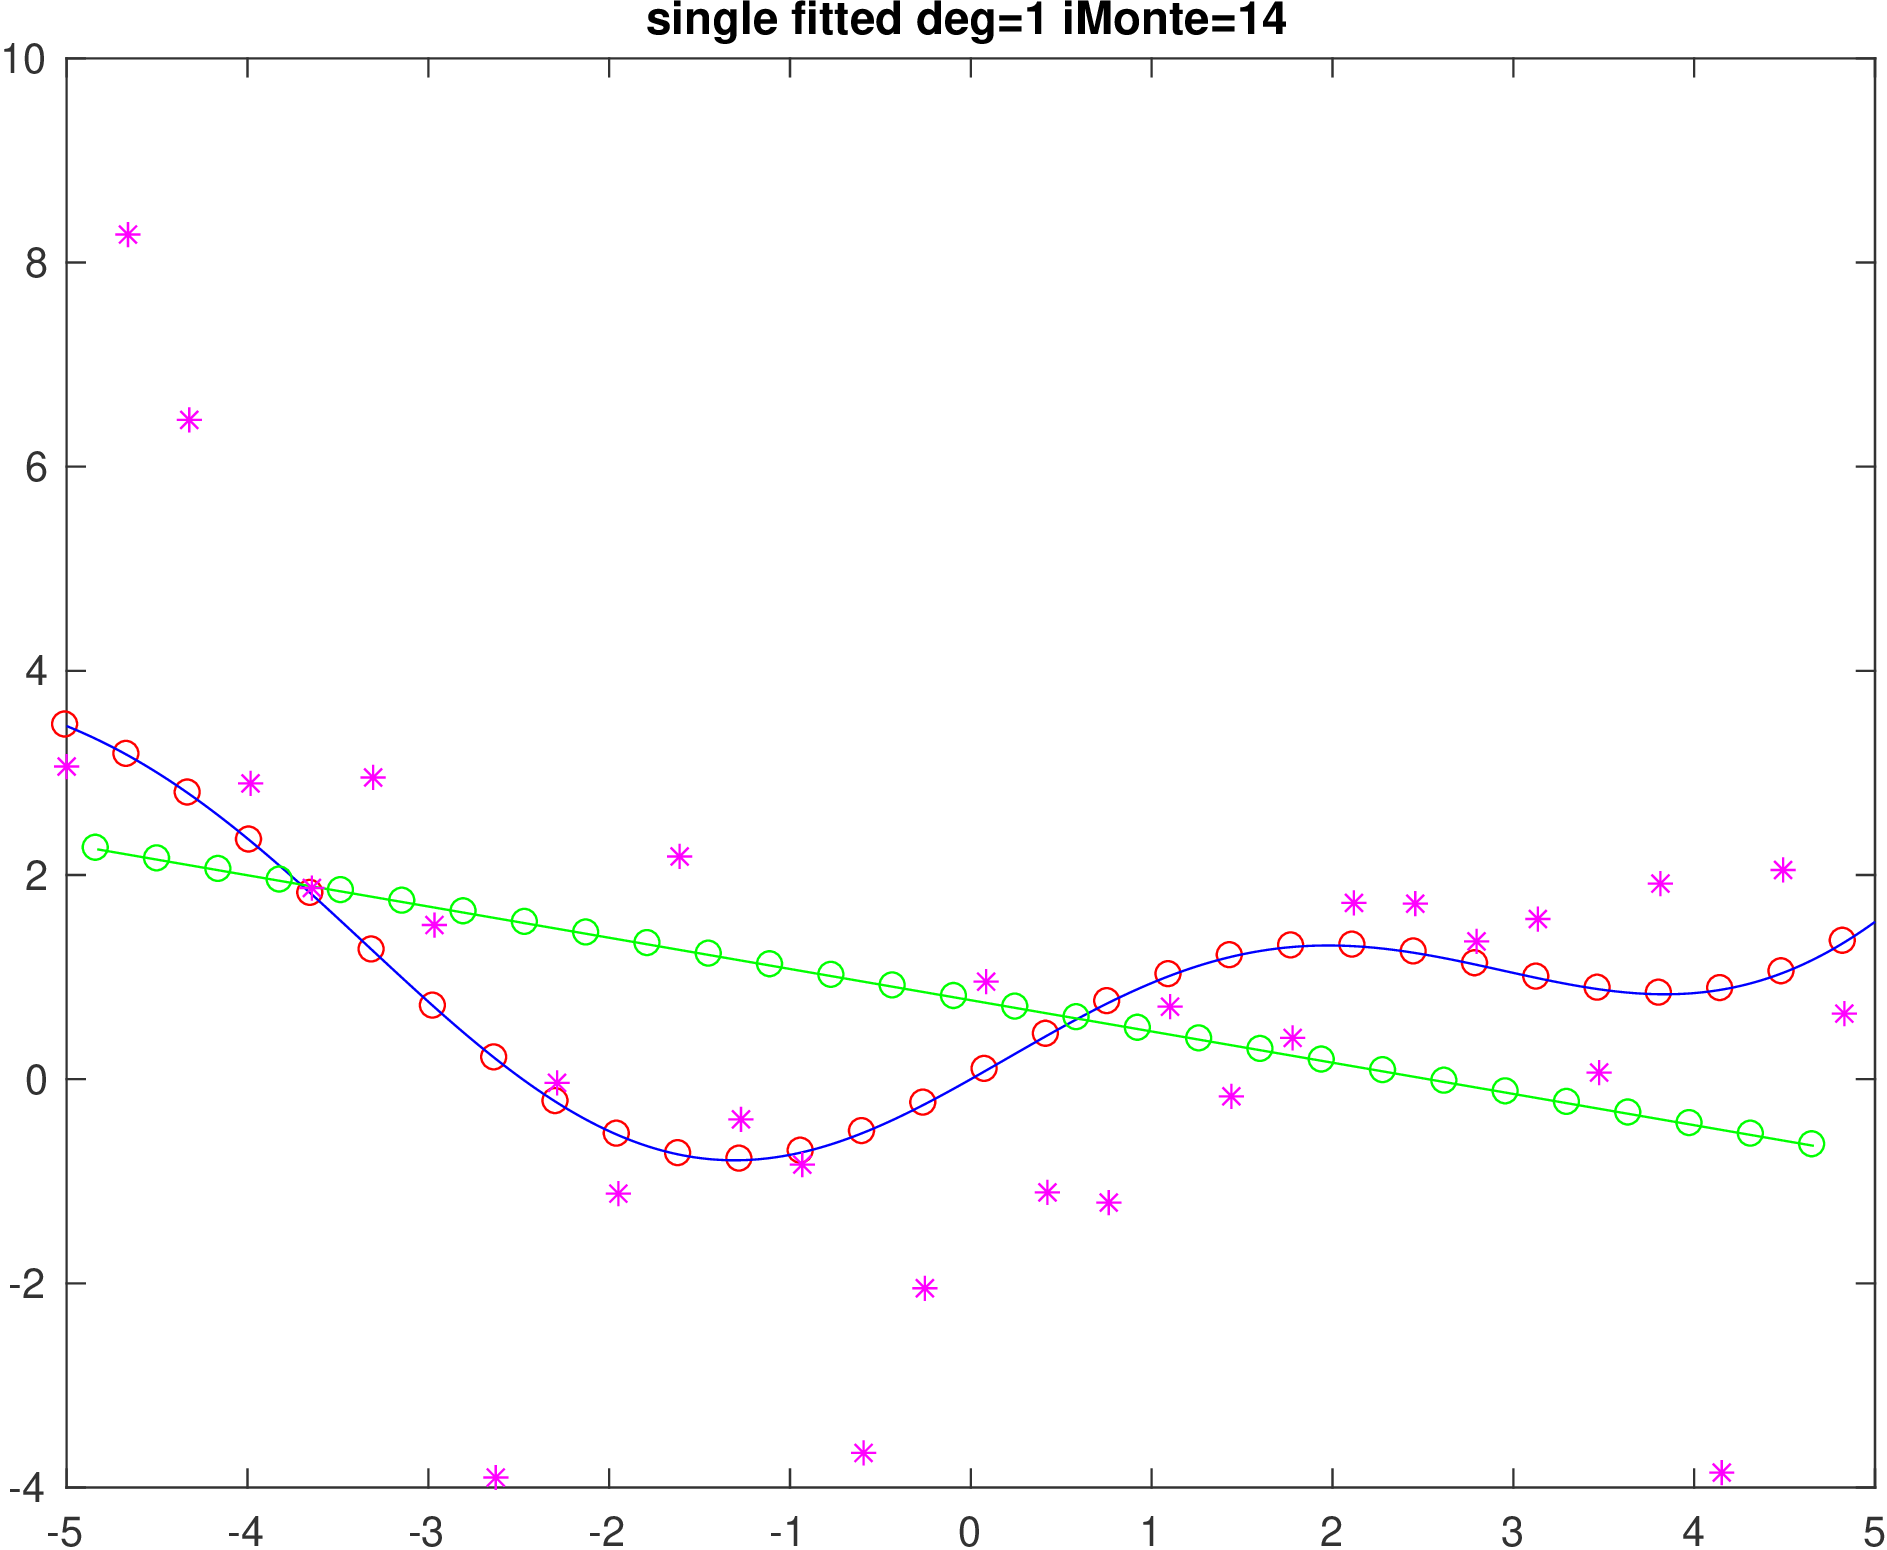
\includegraphics[scale=0.1]{single_poly_d_1_iMonte_14.png}
\end{figure}

\begin{figure}[h!]
\centering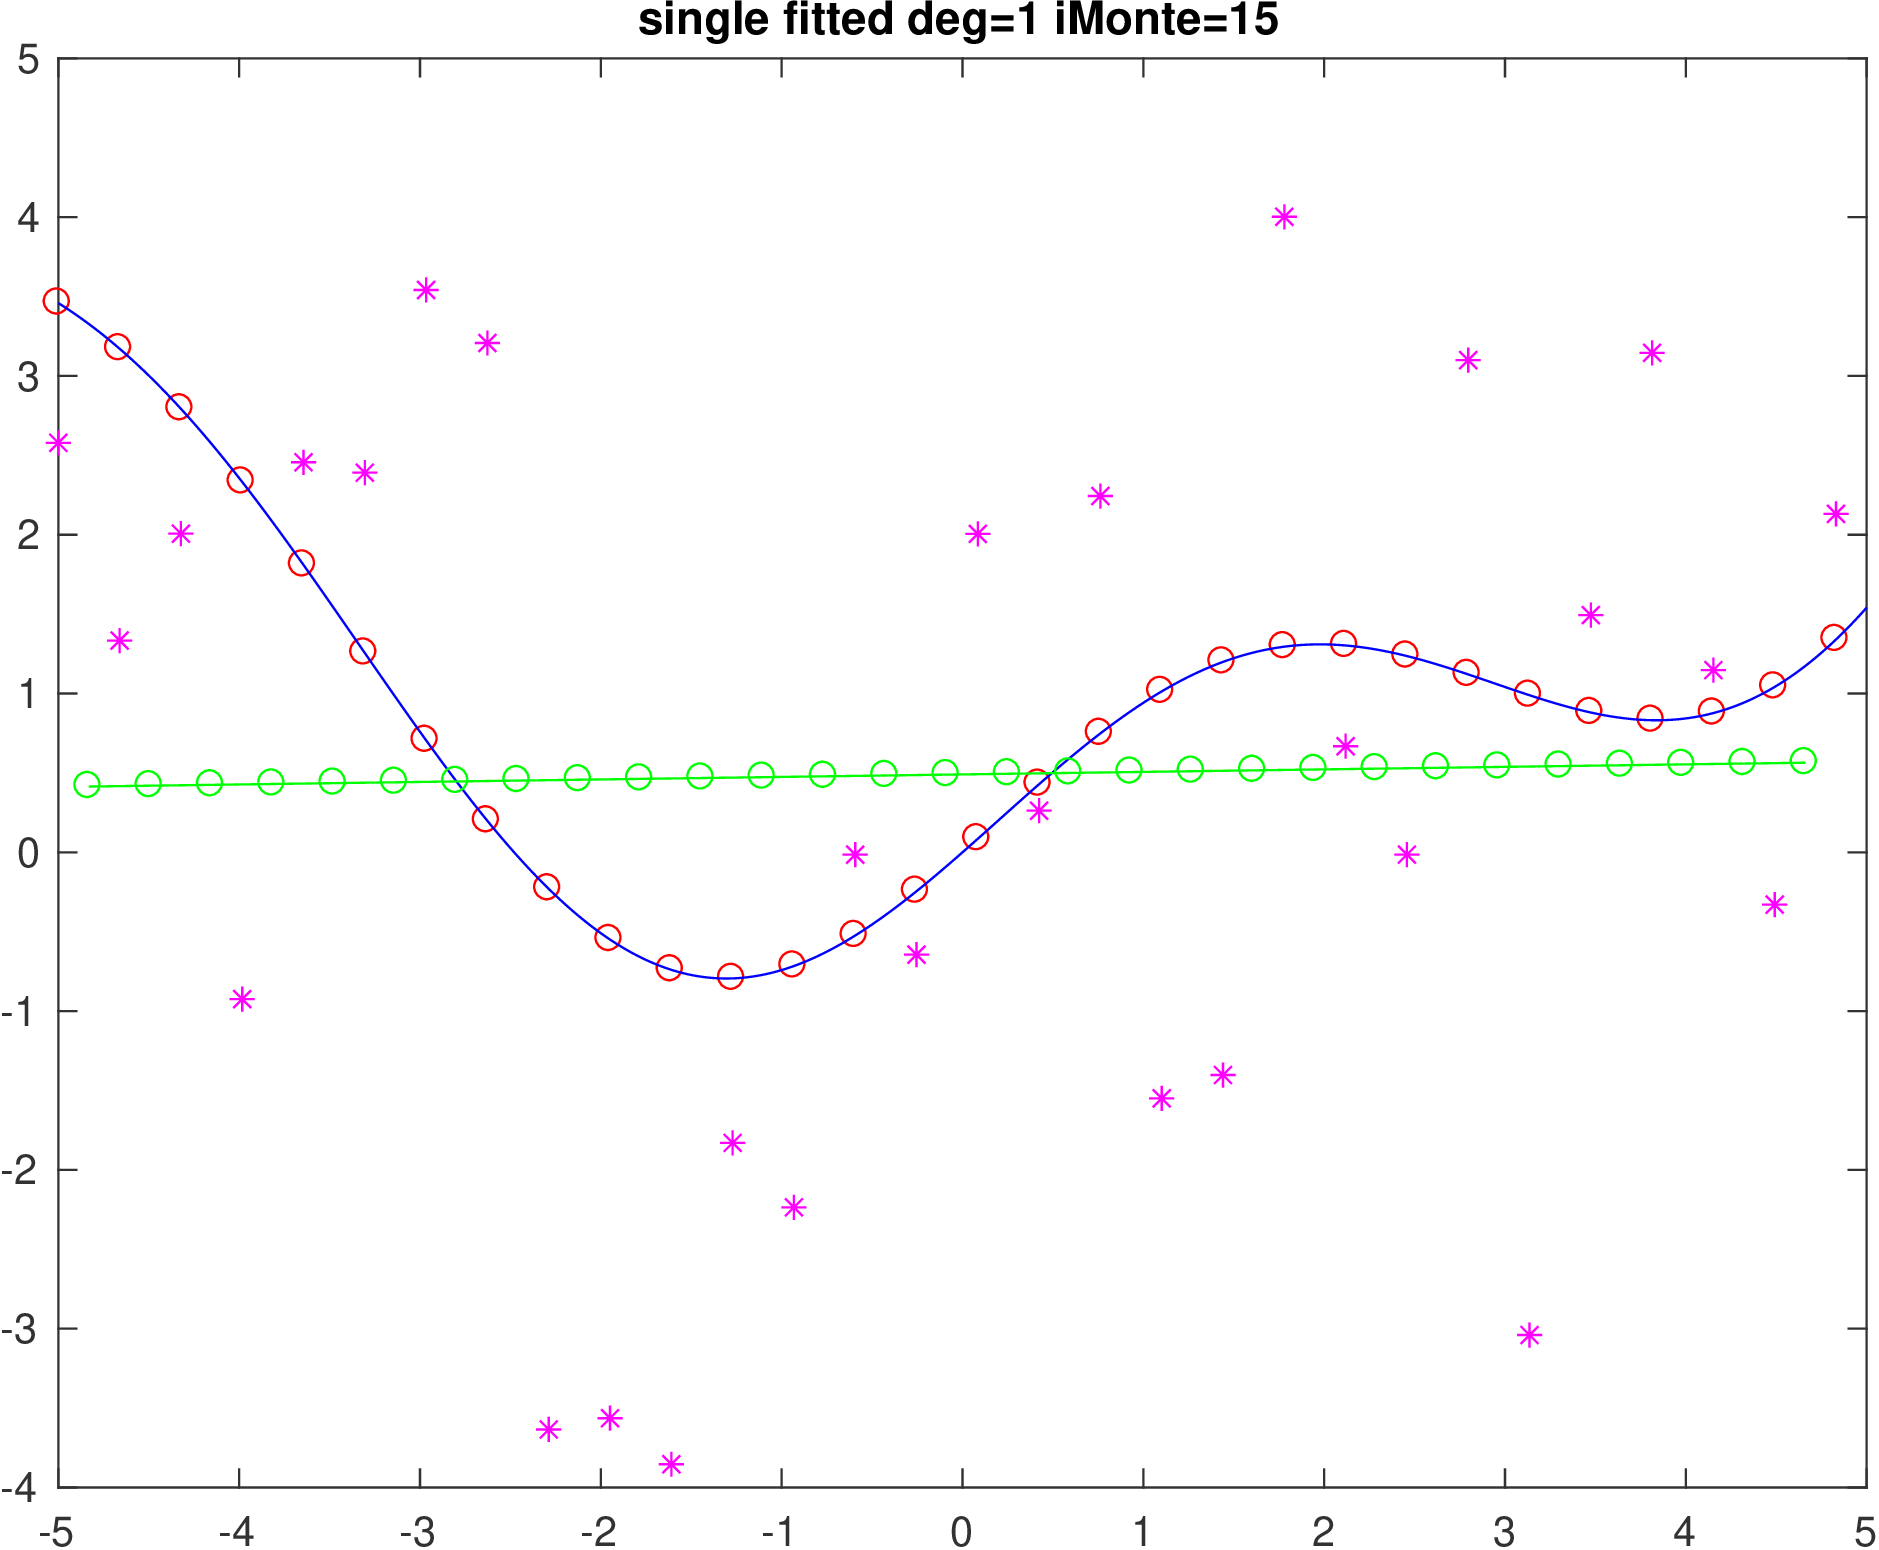
\includegraphics[scale=0.1]{single_poly_d_1_iMonte_15.png}
\end{figure}



\newpage
\subsection{Variance}
The above figures show that for different random draws of noise, the fitted polynomial $\hat{p}$ is different.  That's expected: {\bf When the labels $y_i$ are random, the prediction rule we learn, $h_S$, is also random}
What will cause $h_S$ to have more variance?  Clearly, the higher the noise level, the more variance in $h_S$. But is there anything else? What happens to the variance when we take a larger hypothesis class?

Let's have a look:




\begin{figure}[h!]
\centering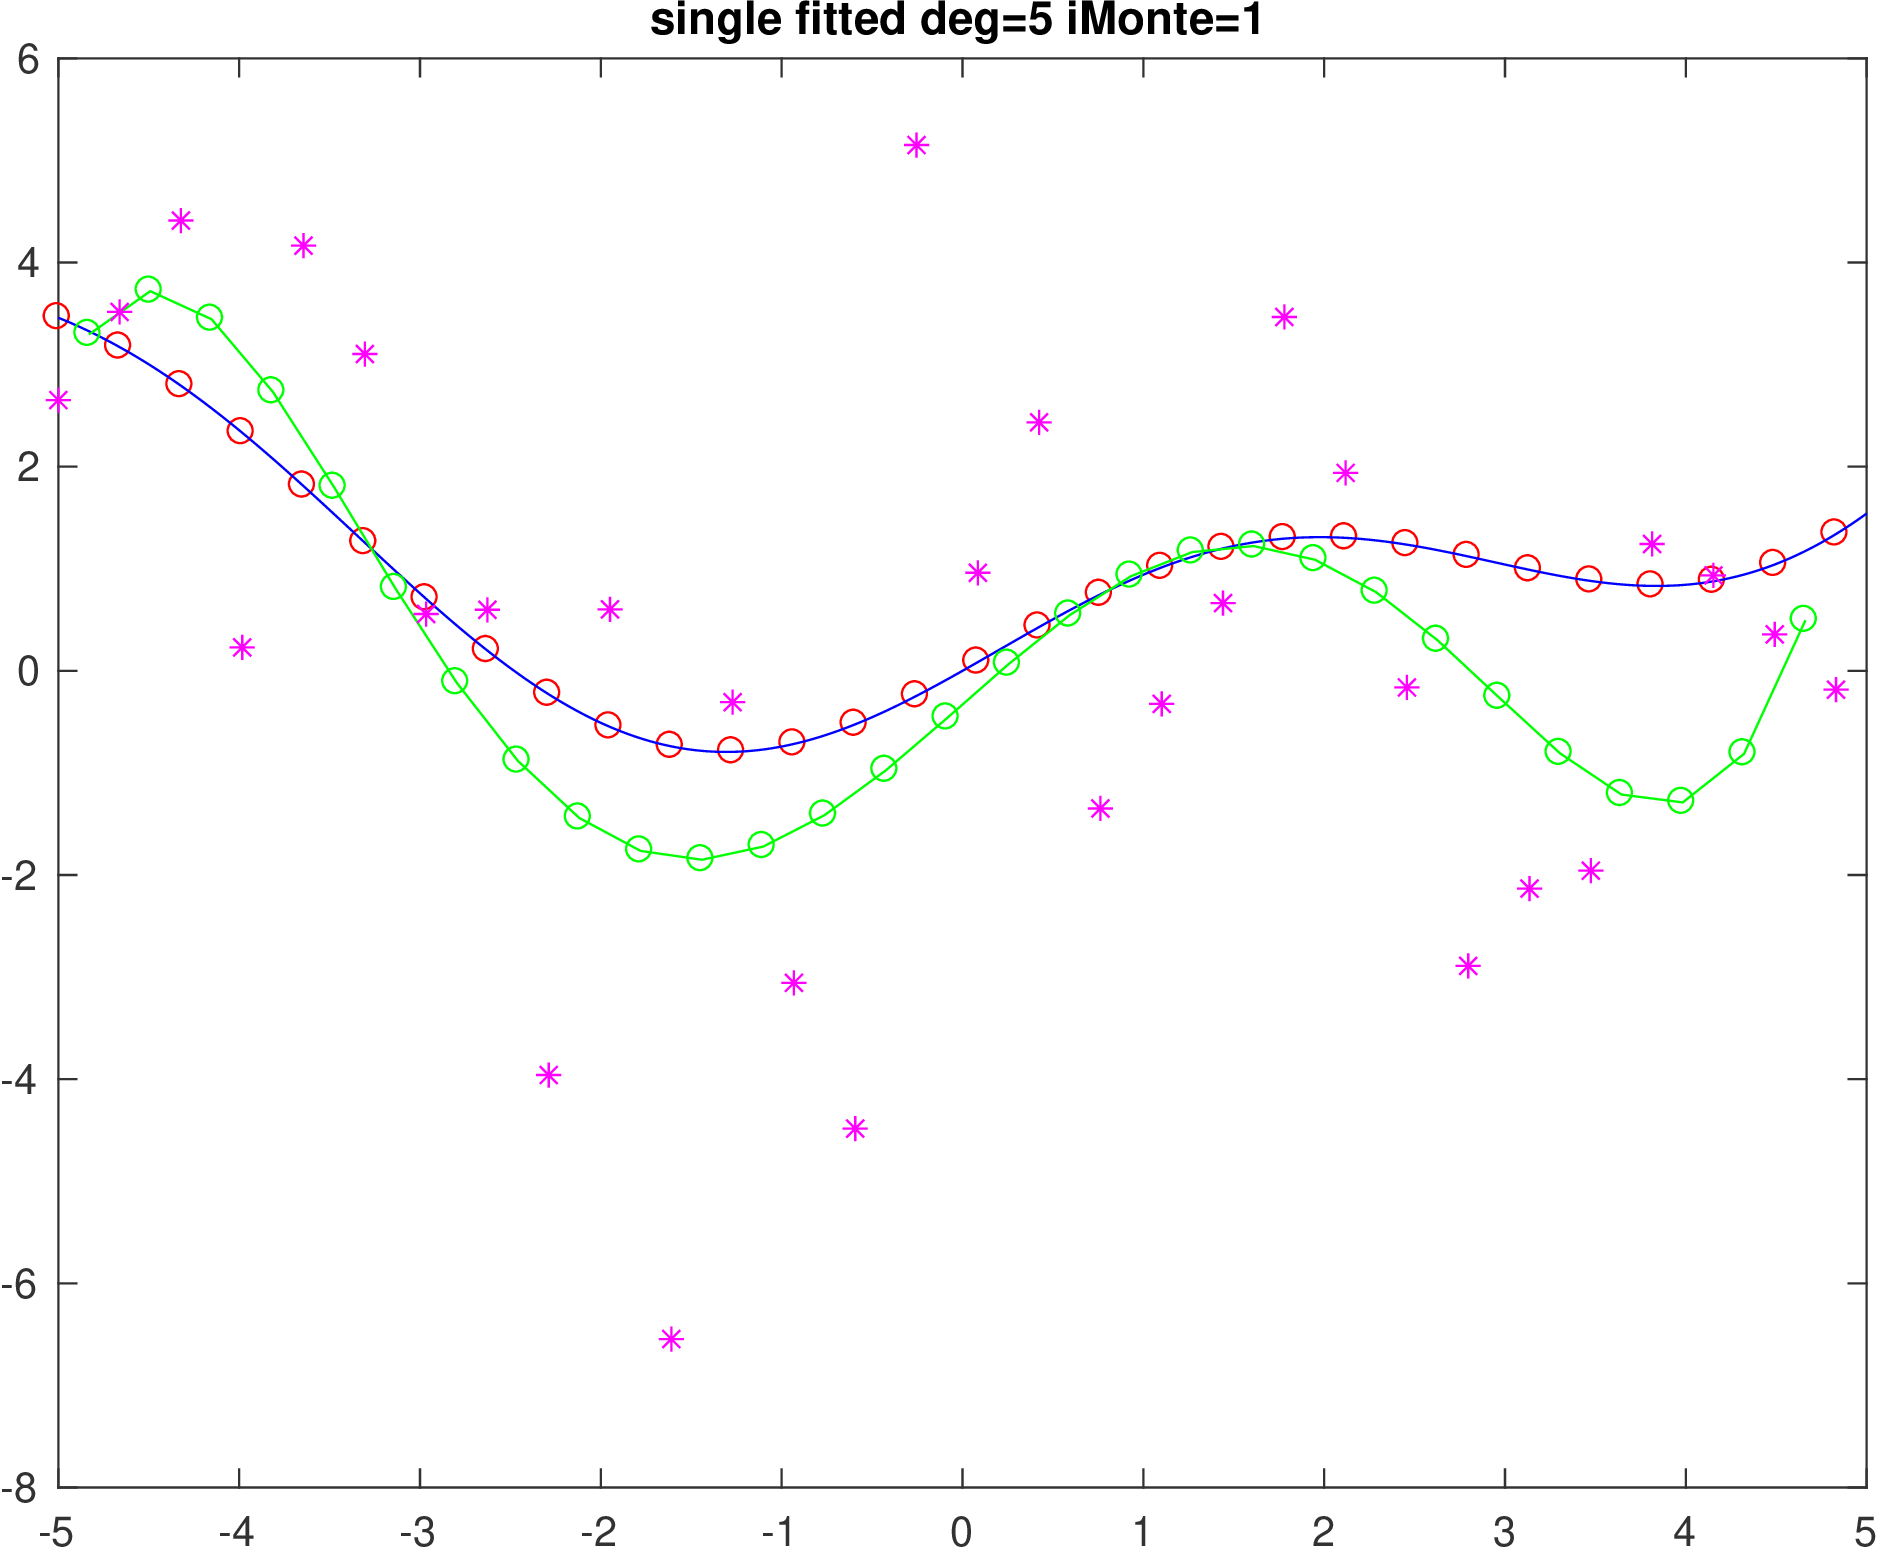
\includegraphics[scale=0.1]{single_poly_d_5_iMonte_1.png}
\end{figure}

 \begin{figure}[h!]
\centering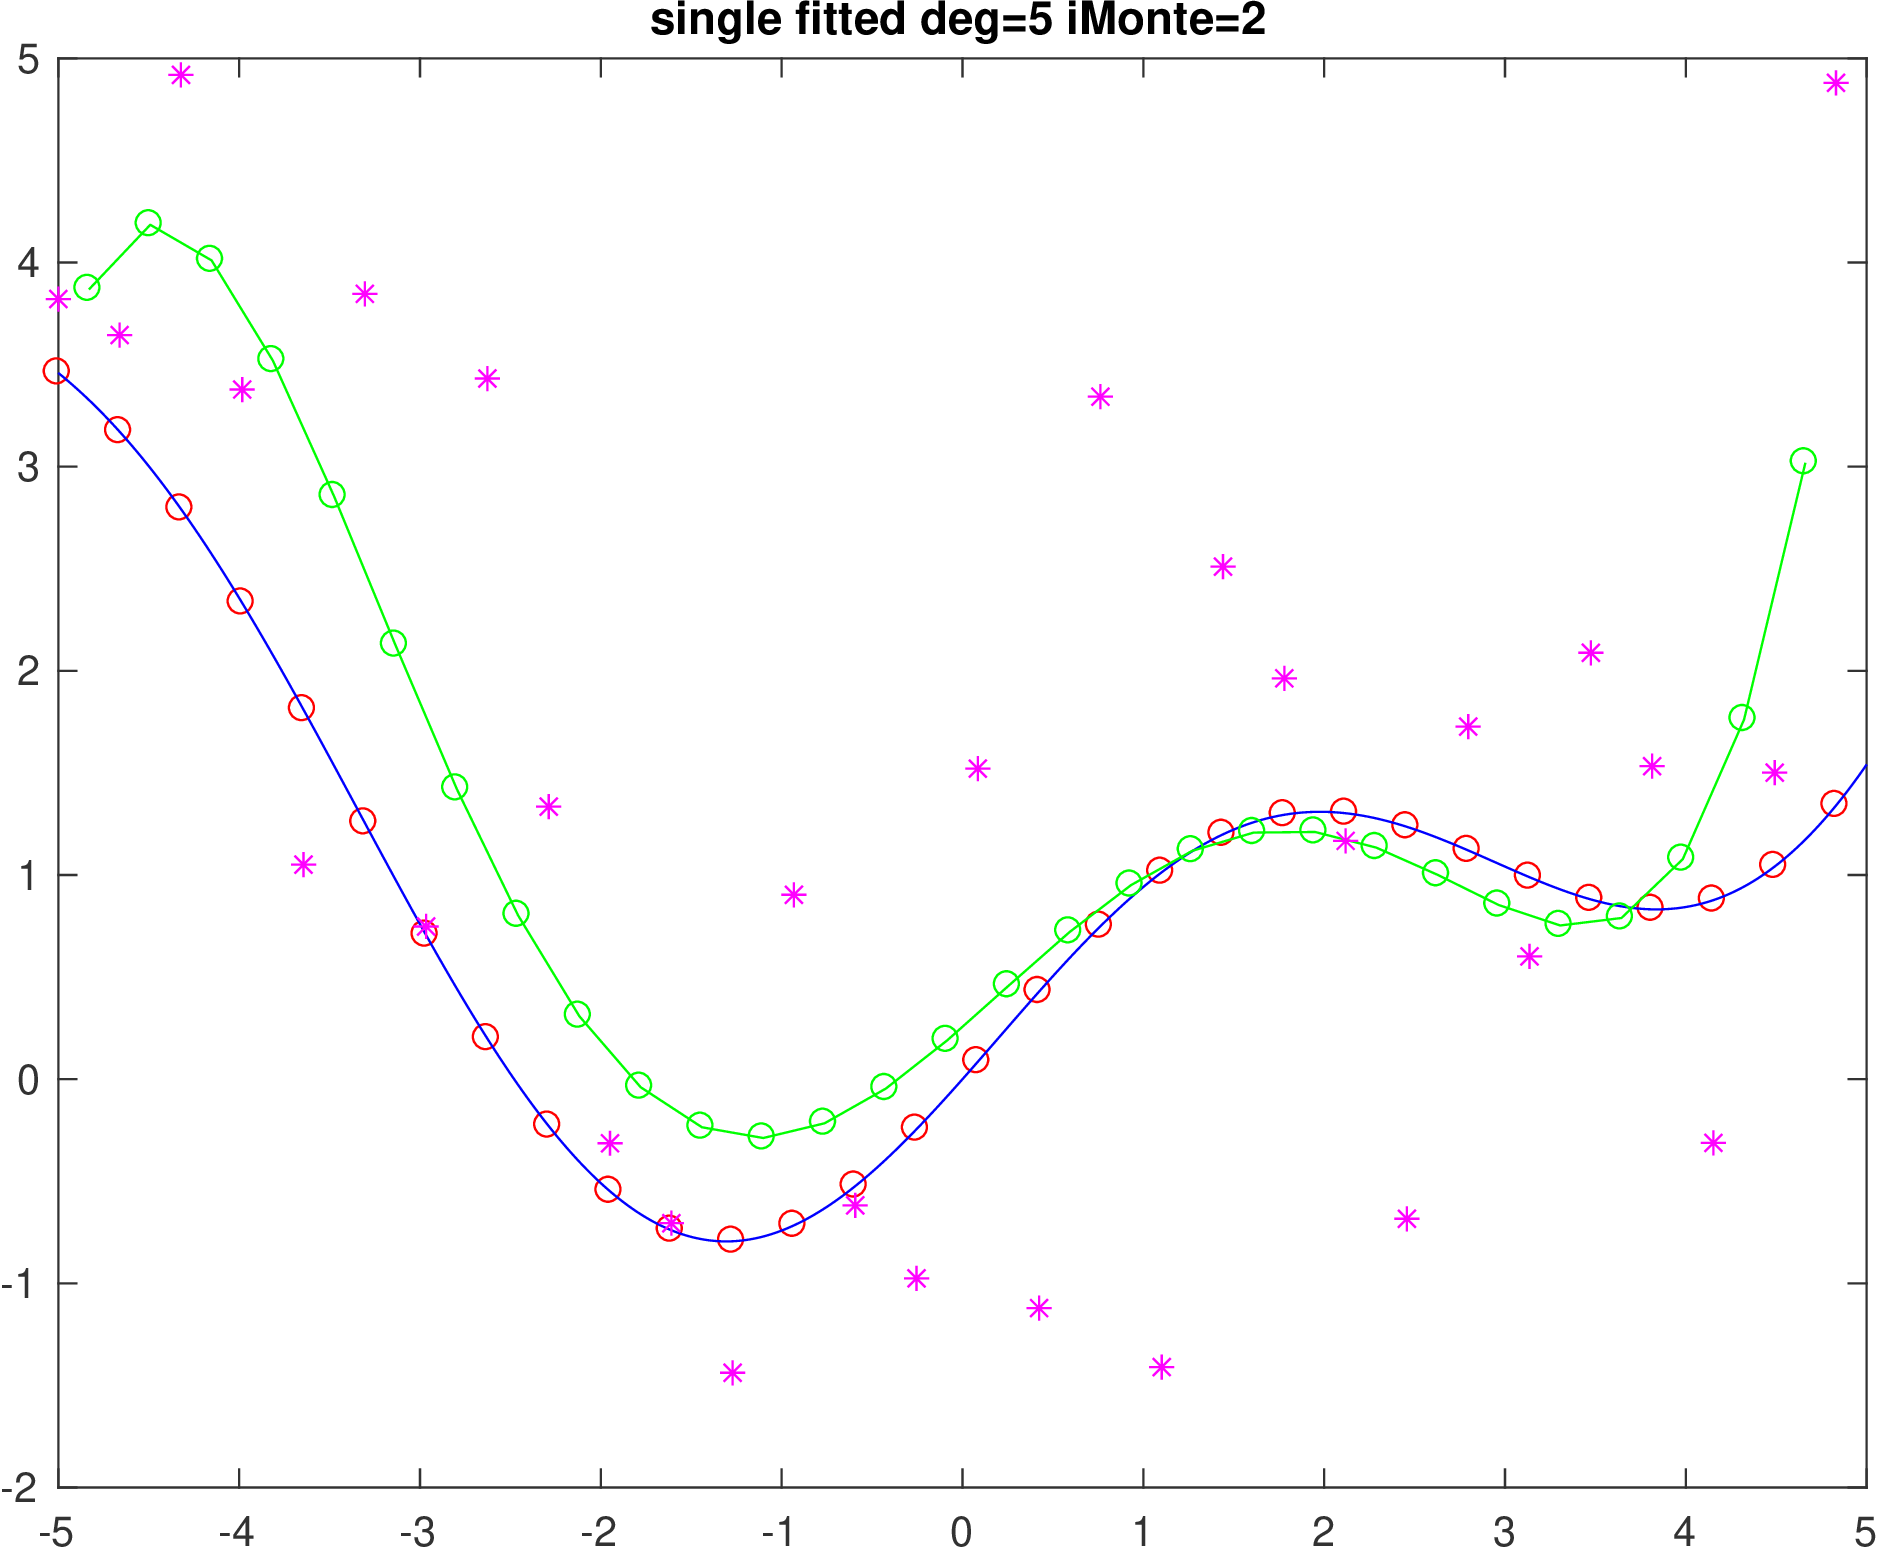
\includegraphics[scale=0.1]{single_poly_d_5_iMonte_2.png}
\end{figure}

\begin{figure}[h!]
\centering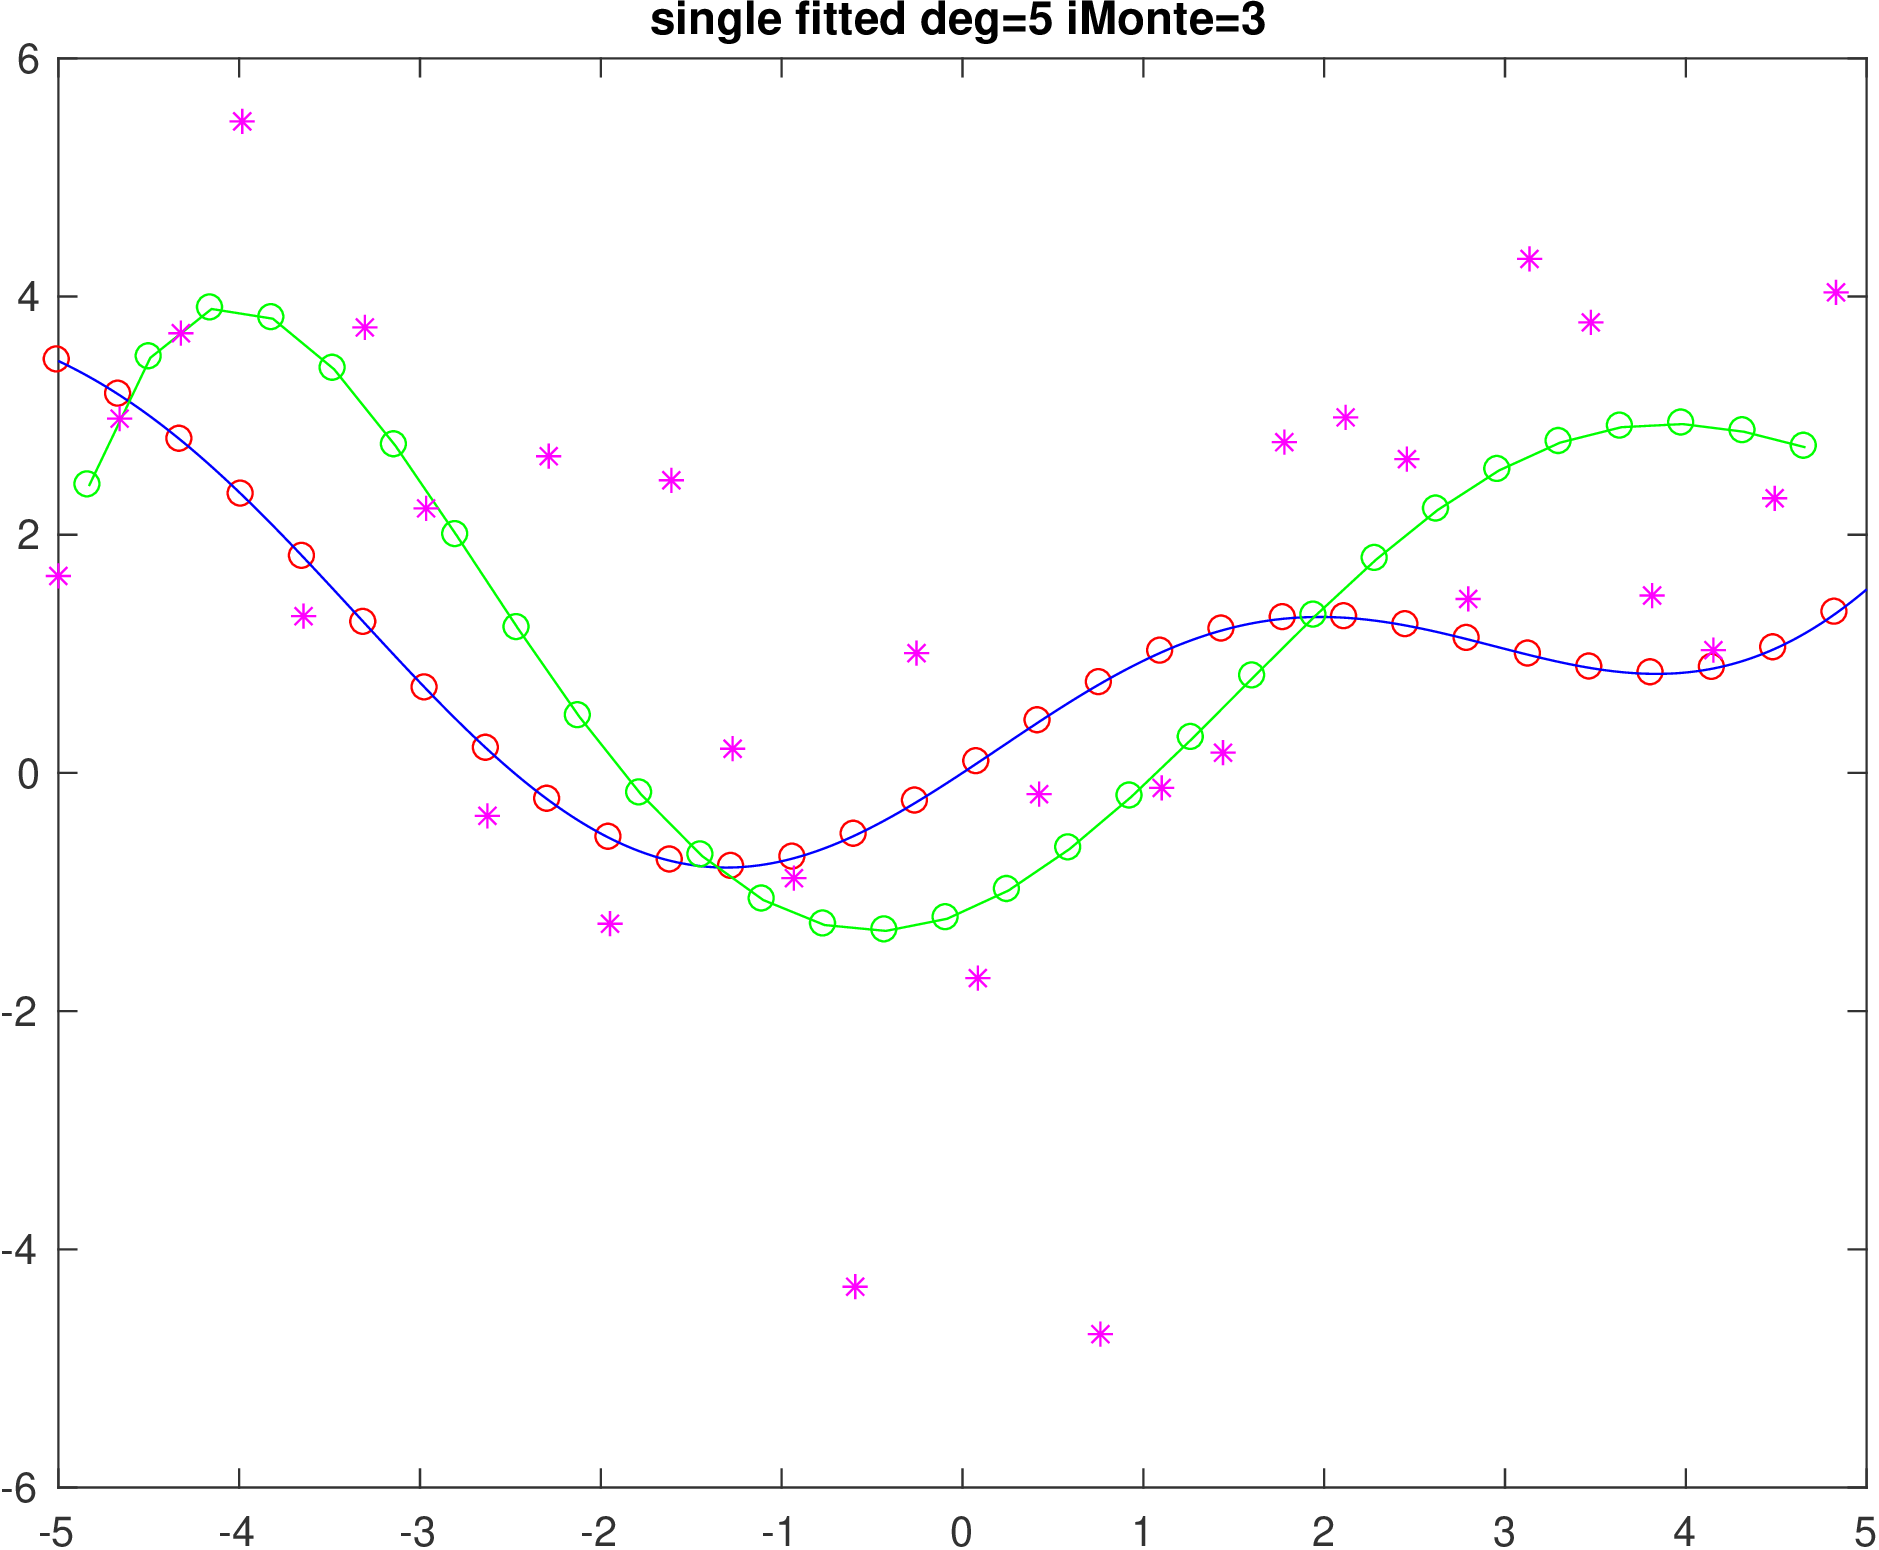
\includegraphics[scale=0.1]{single_poly_d_5_iMonte_3.png}
\end{figure}

\begin{figure}[h!]
\centering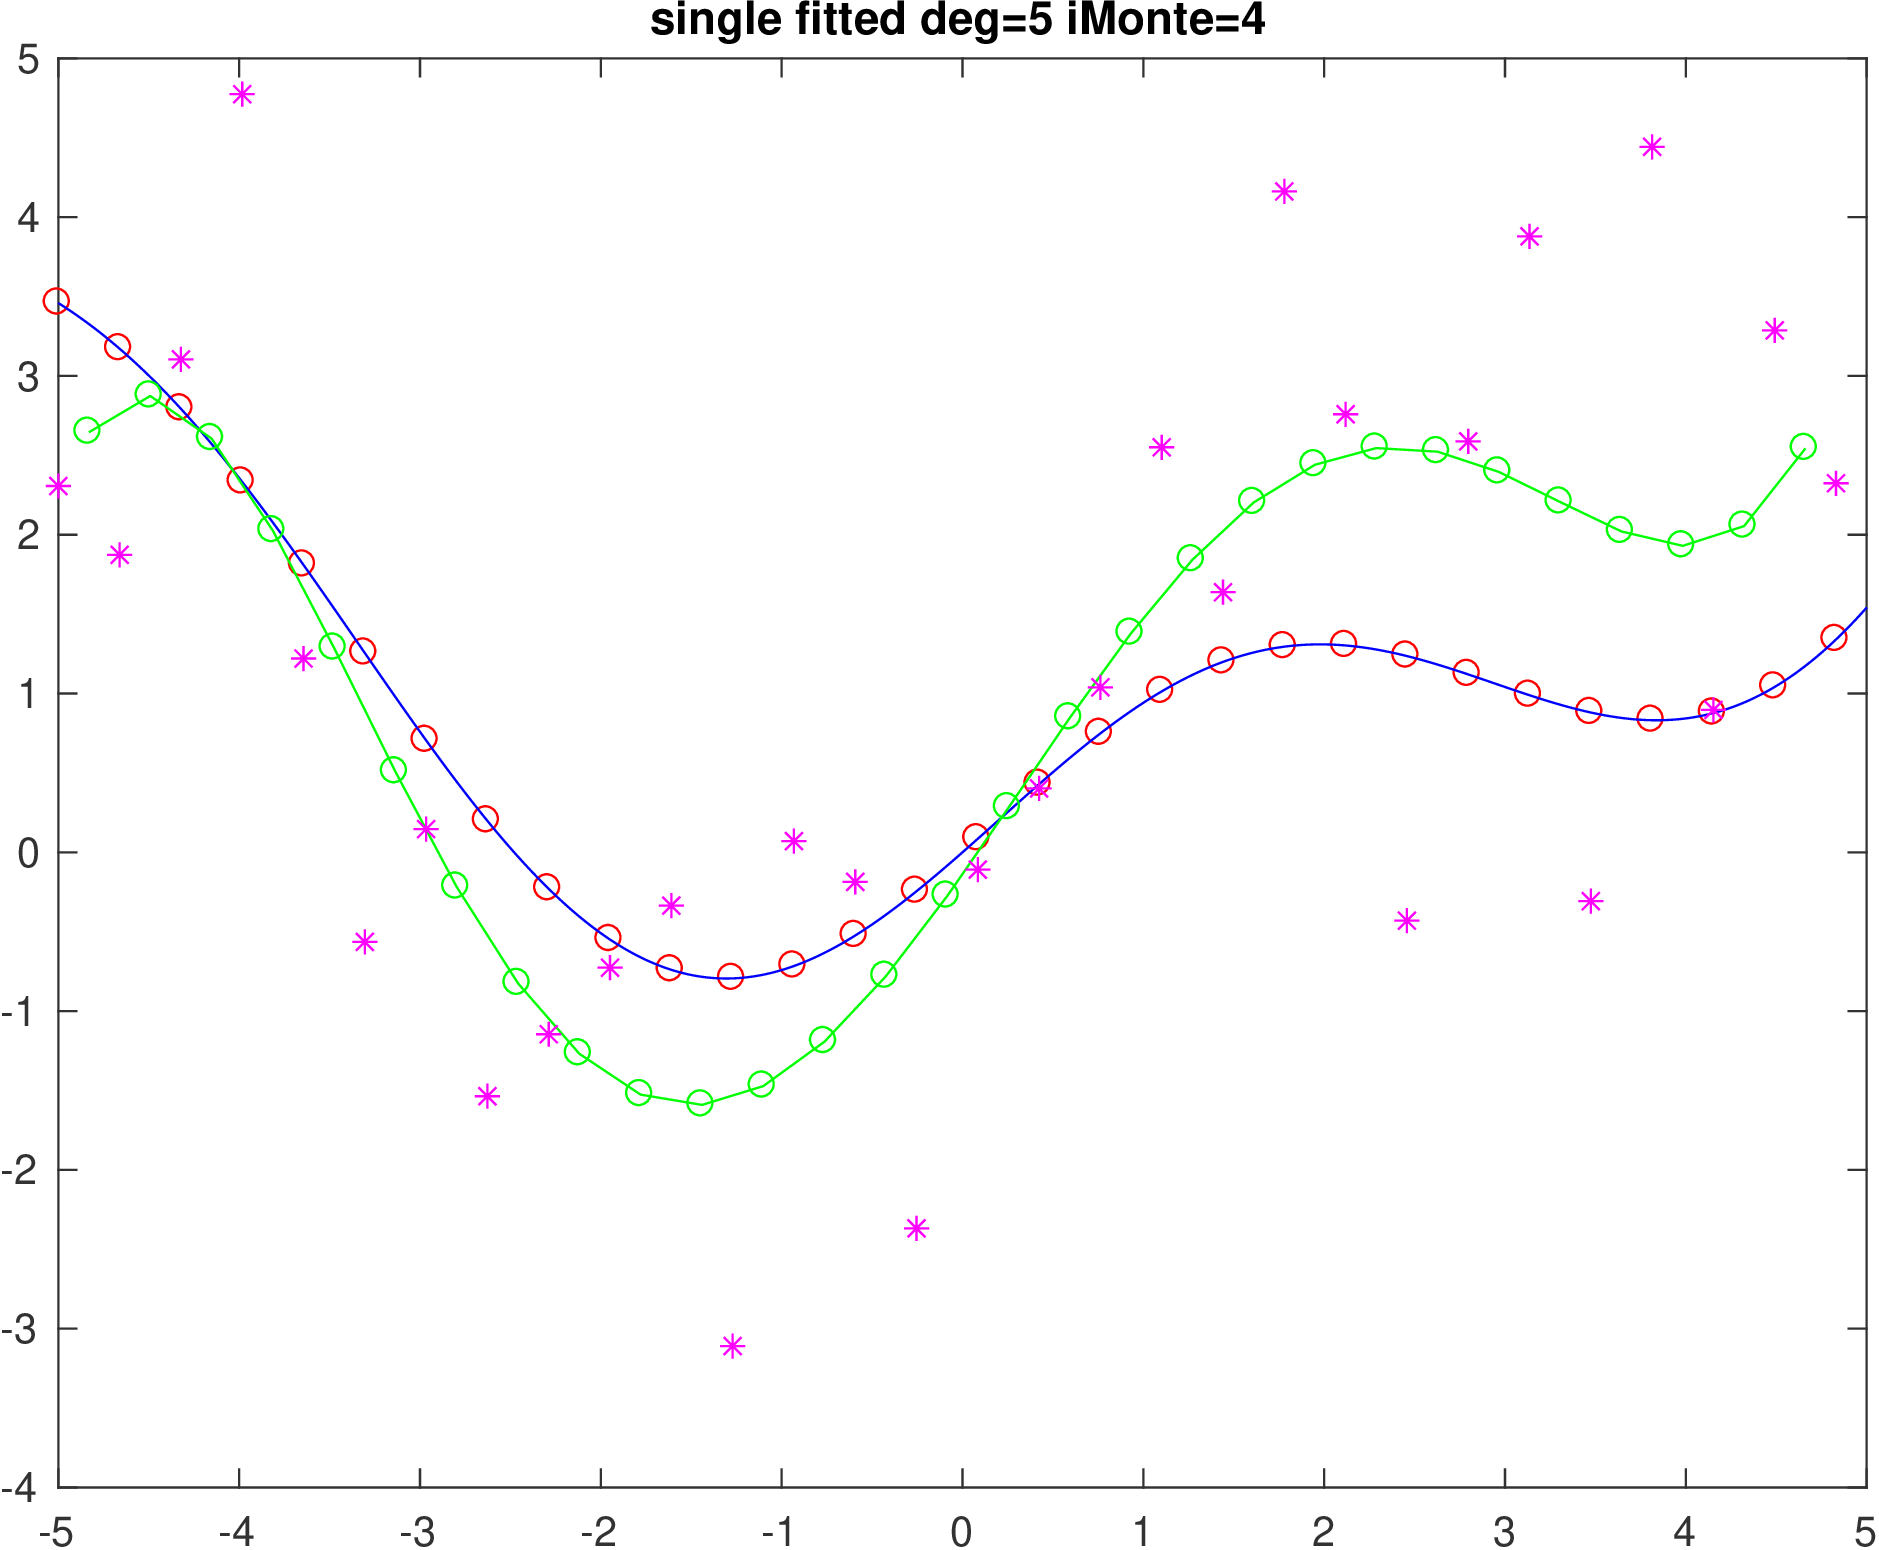
\includegraphics[scale=0.1]{single_poly_d_5_iMonte_4.png}
\end{figure}


\begin{figure}[h!]
\centering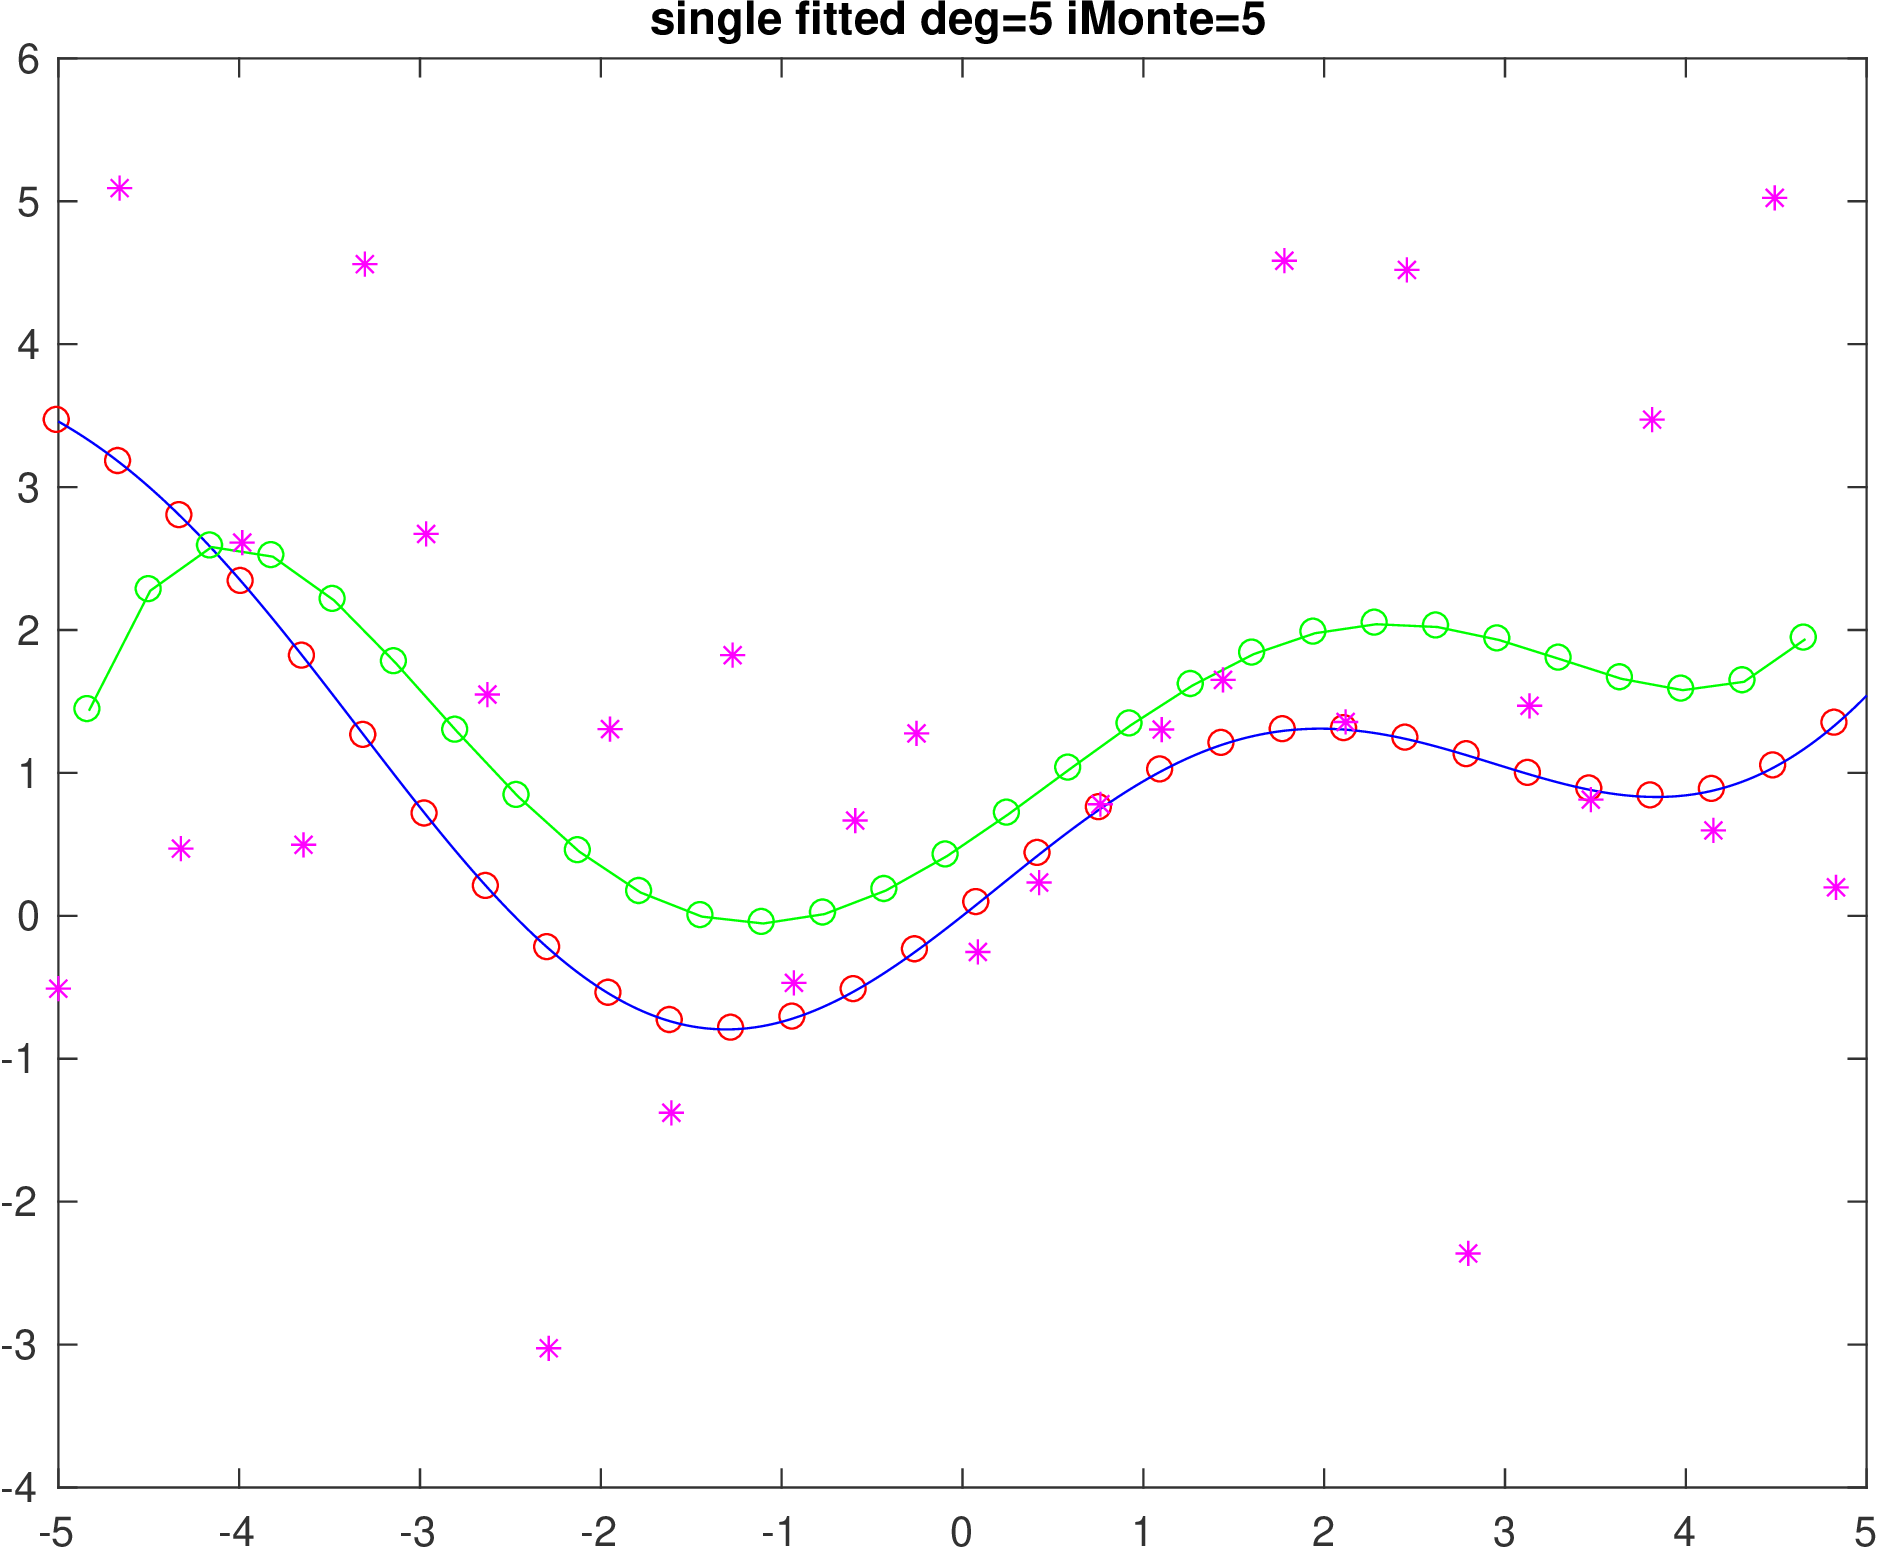
\includegraphics[scale=0.1]{single_poly_d_5_iMonte_5.png}
\end{figure}


\begin{figure}[h!]
\centering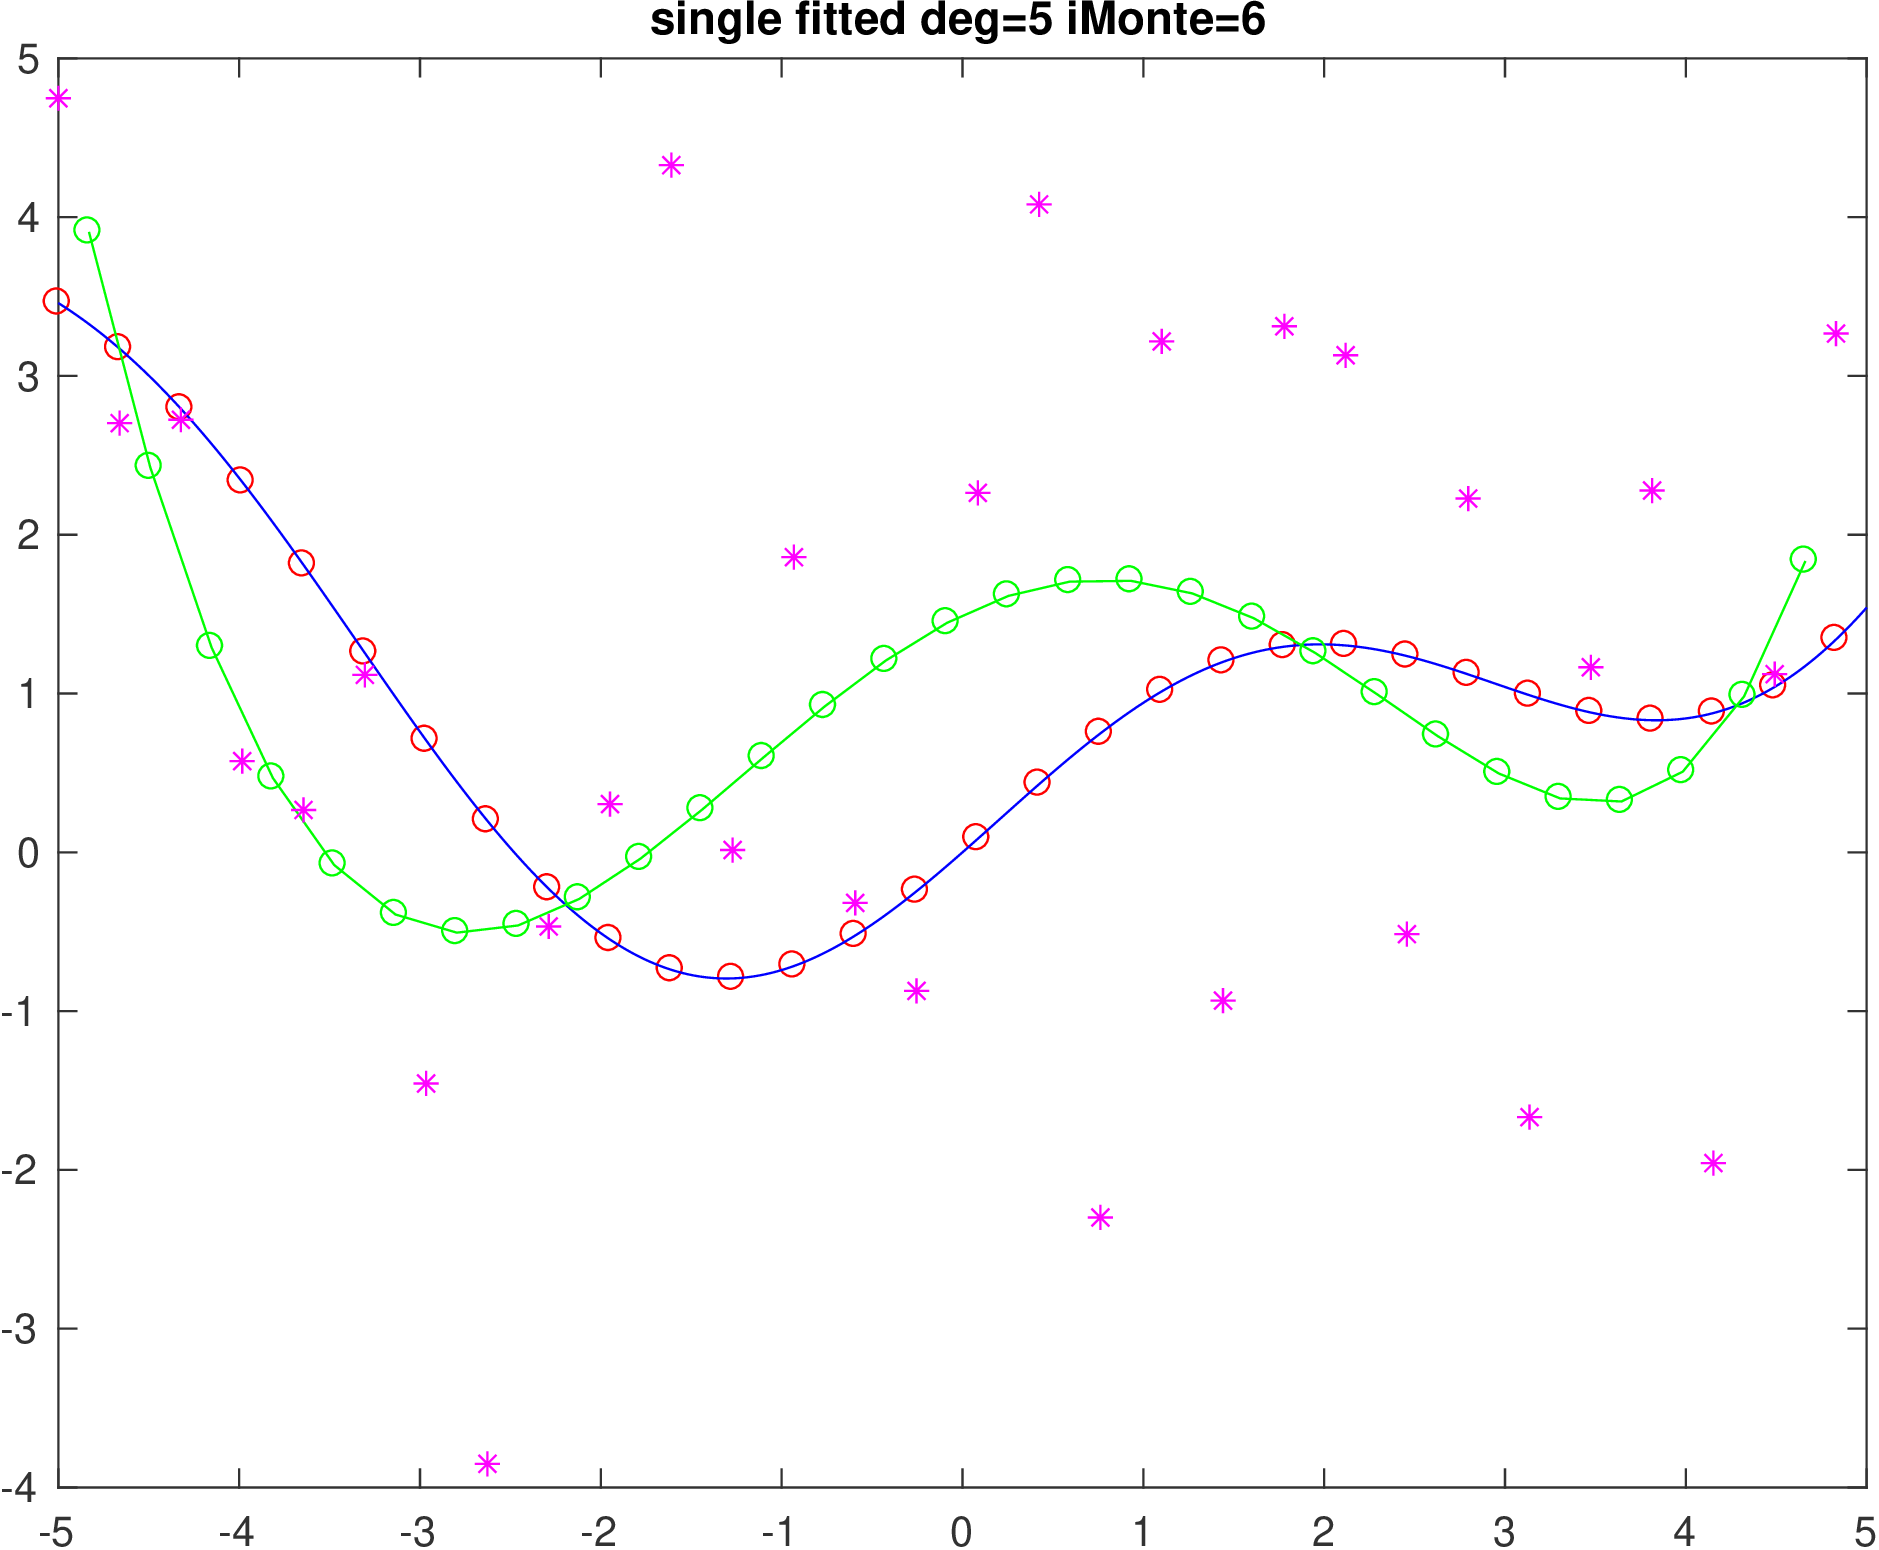
\includegraphics[scale=0.1]{single_poly_d_5_iMonte_6.png}
\end{figure}

\begin{figure}[h!]
\centering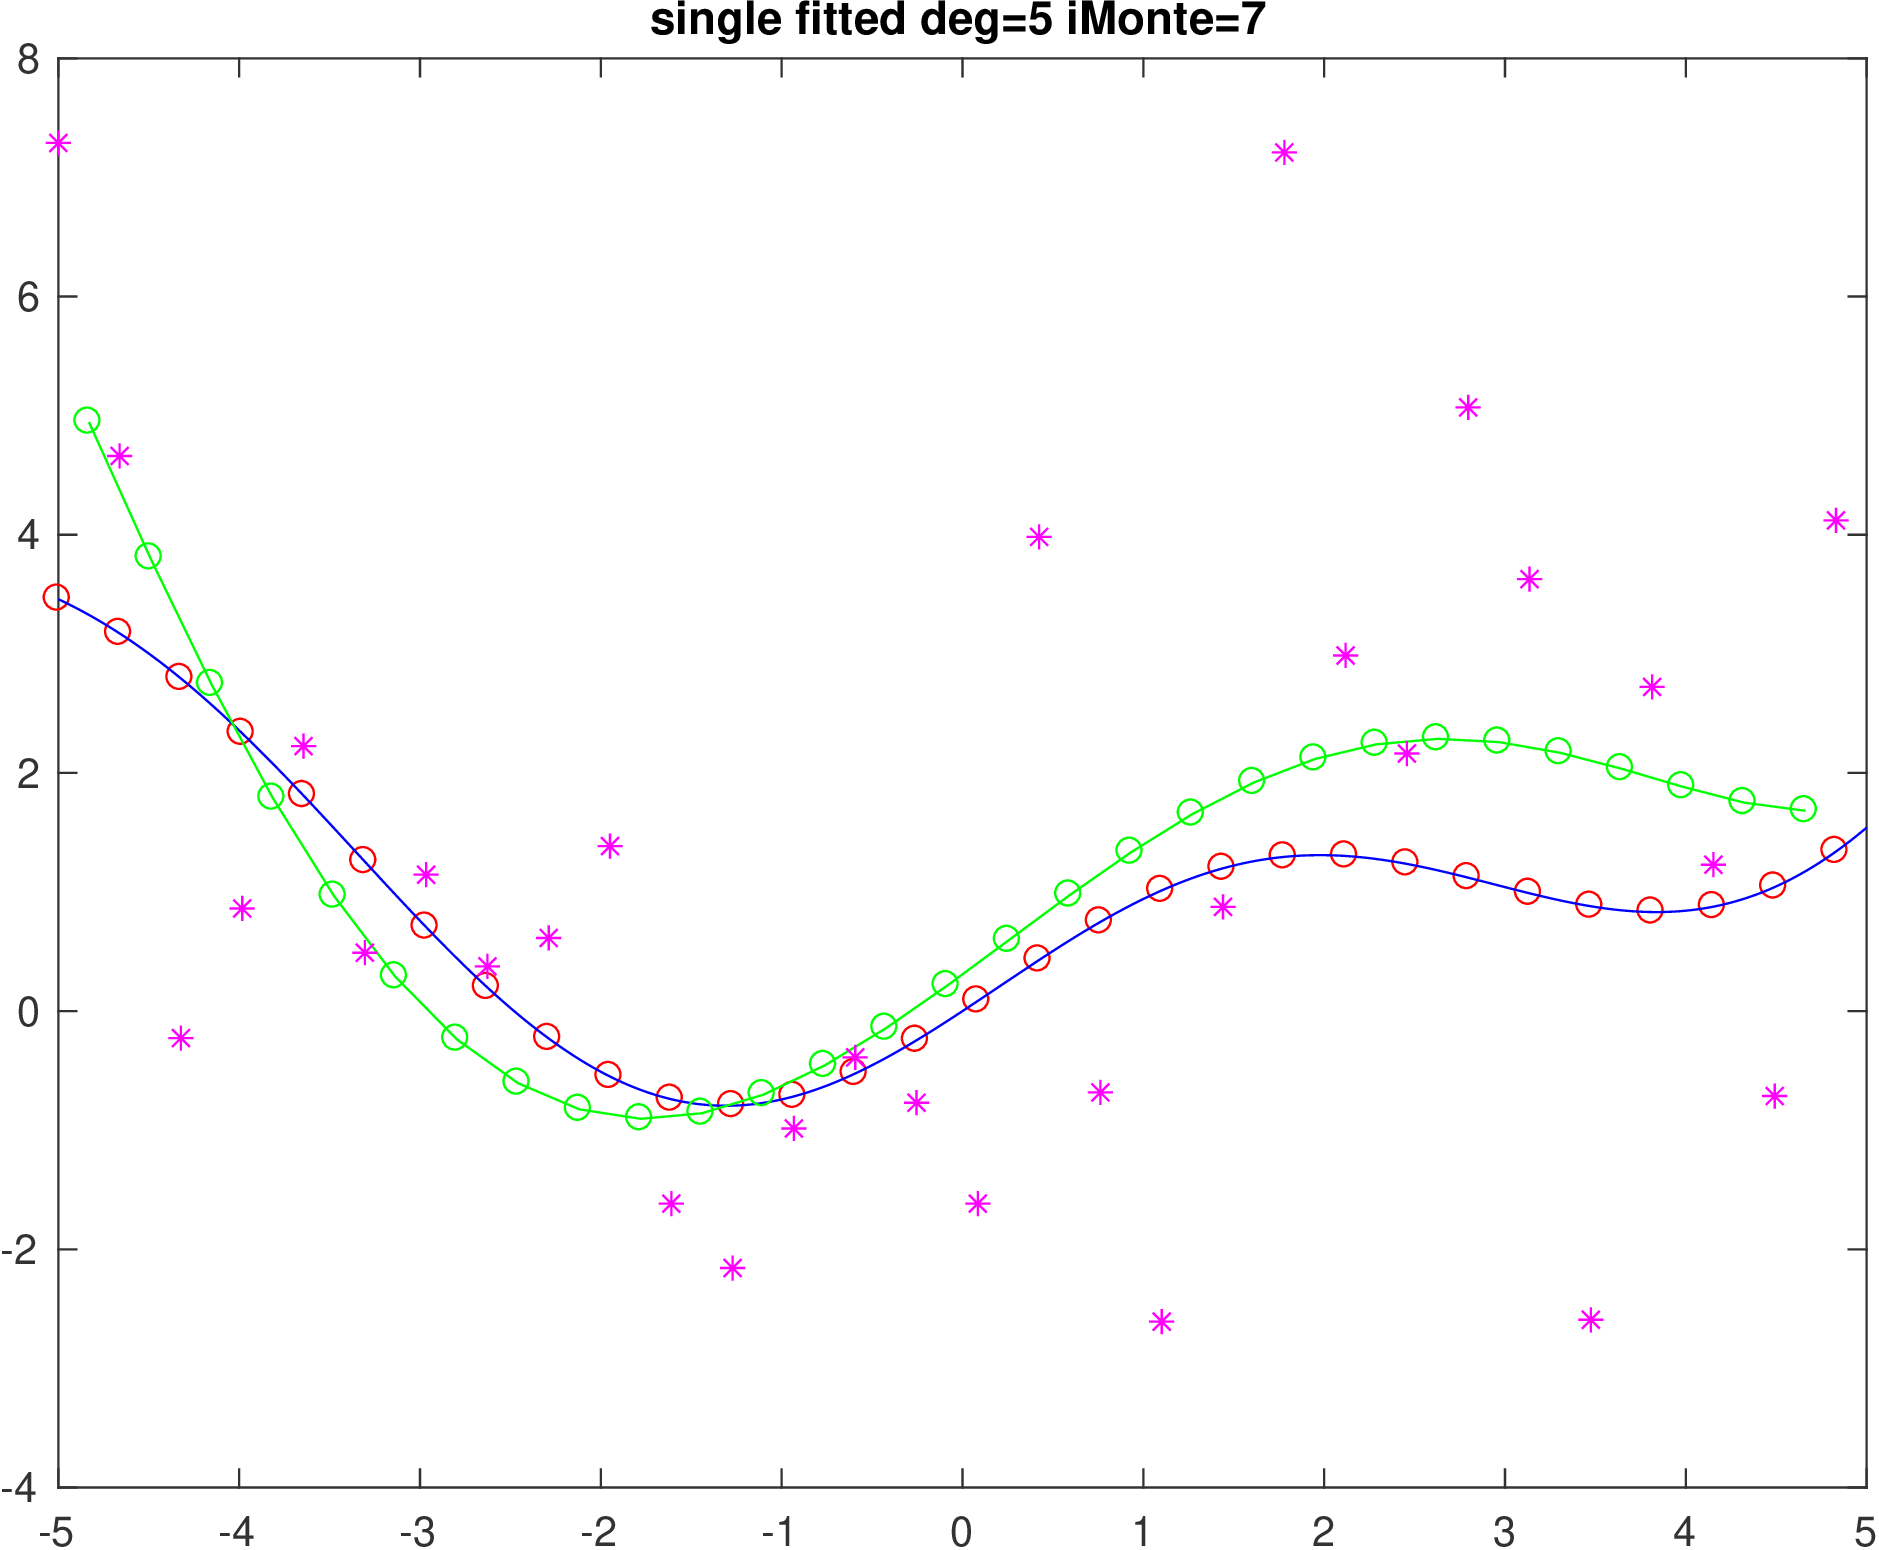
\includegraphics[scale=0.1]{single_poly_d_5_iMonte_7.png}
\end{figure}


\begin{figure}[h!]
\centering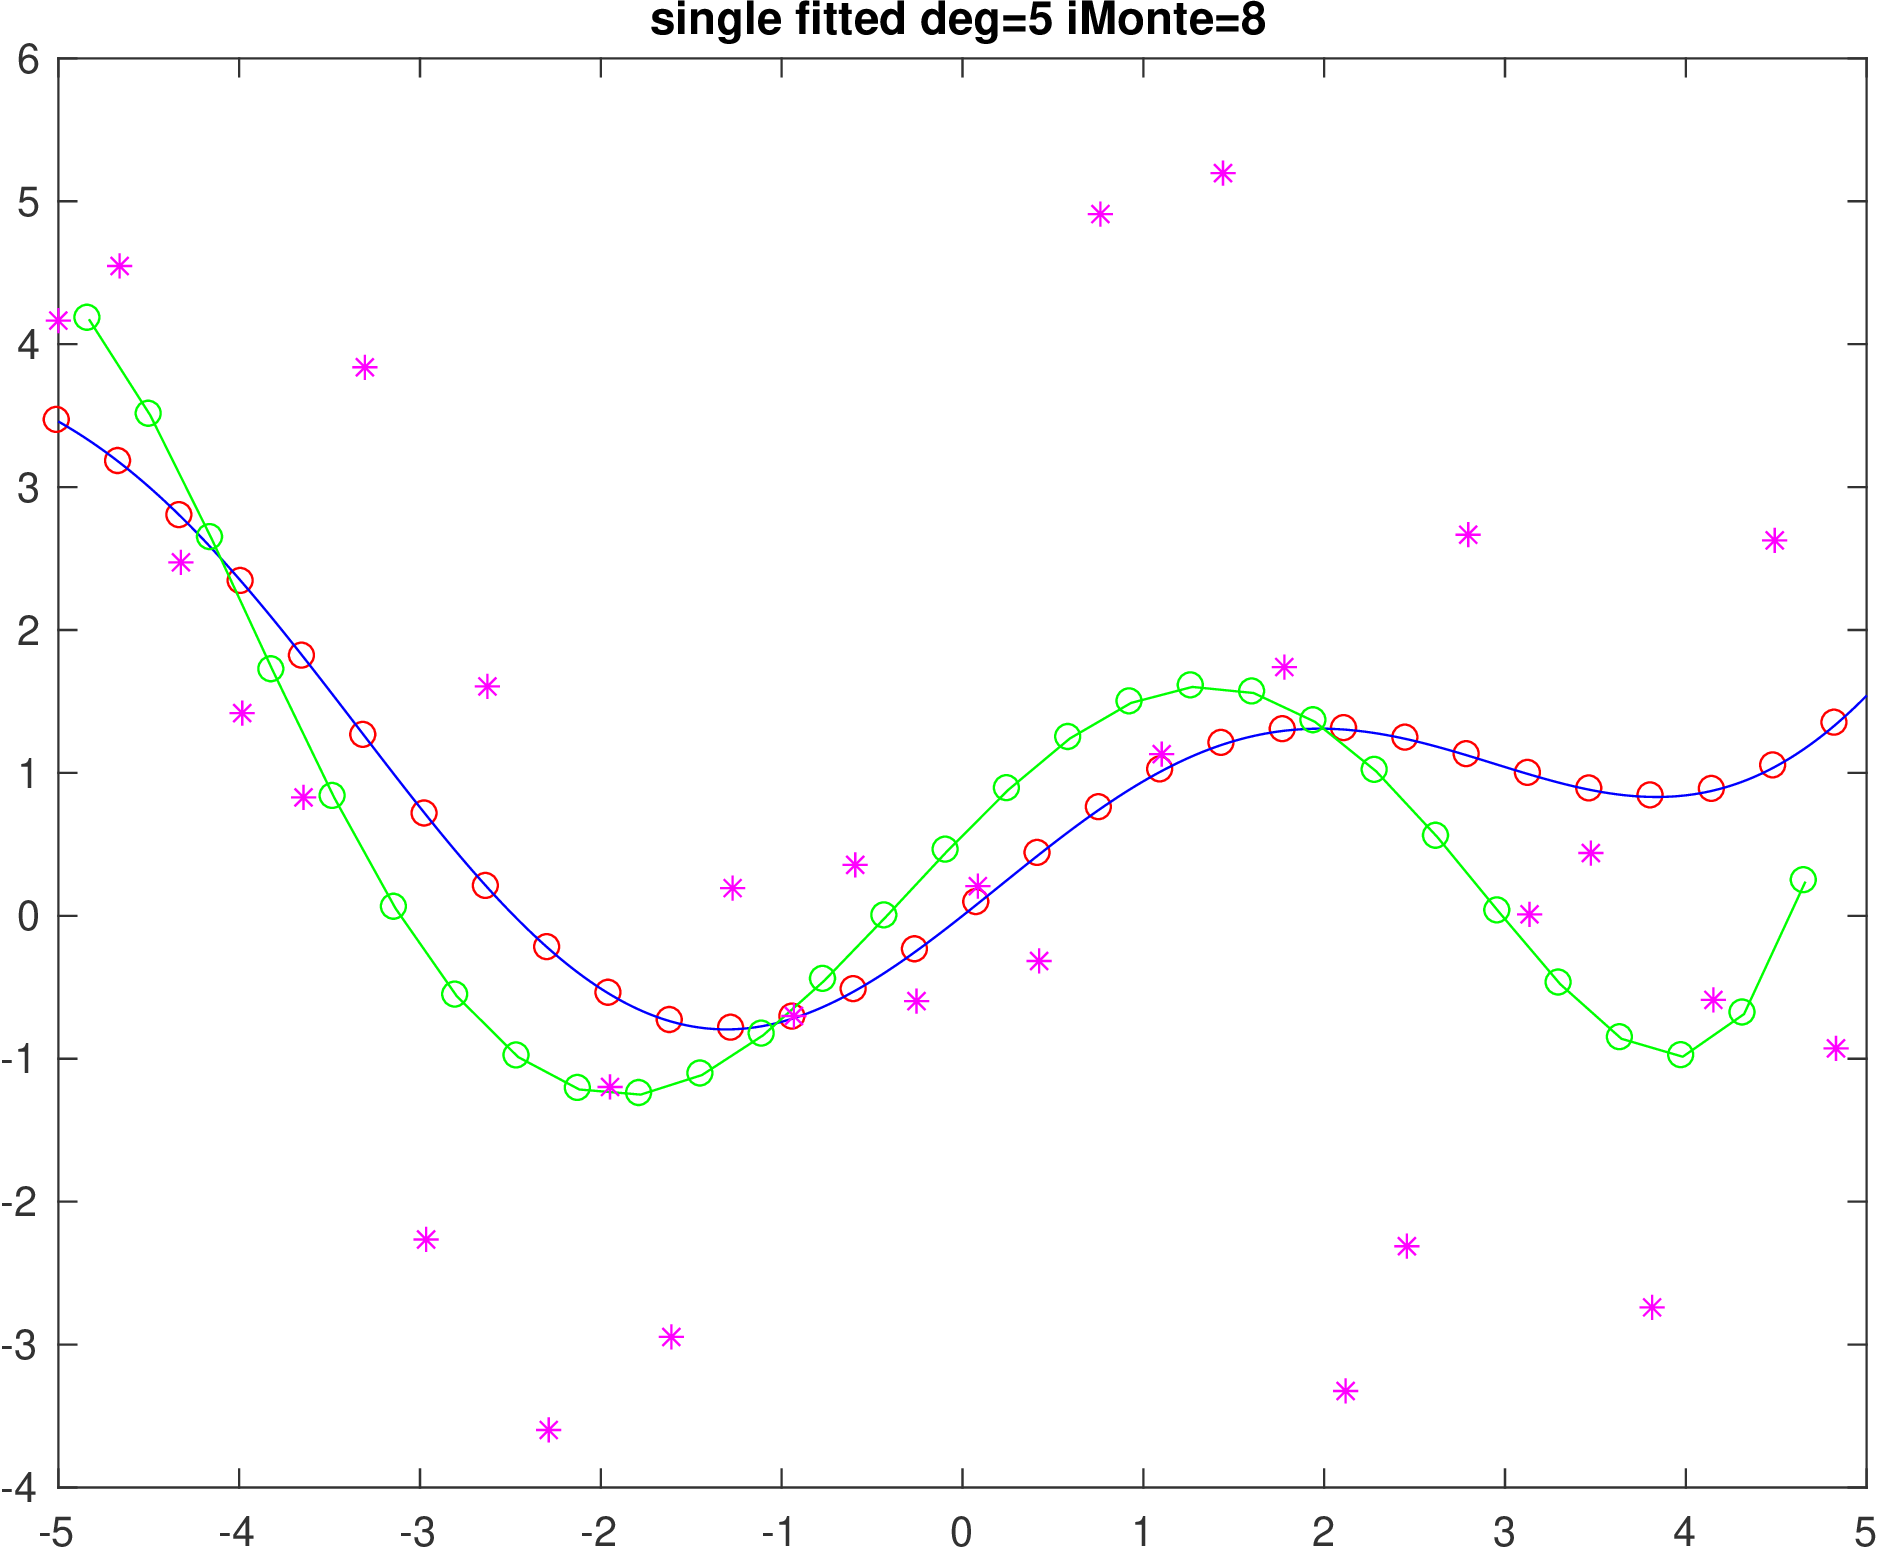
\includegraphics[scale=0.1]{single_poly_d_5_iMonte_8.png}
\end{figure}


\begin{figure}[h!]
\centering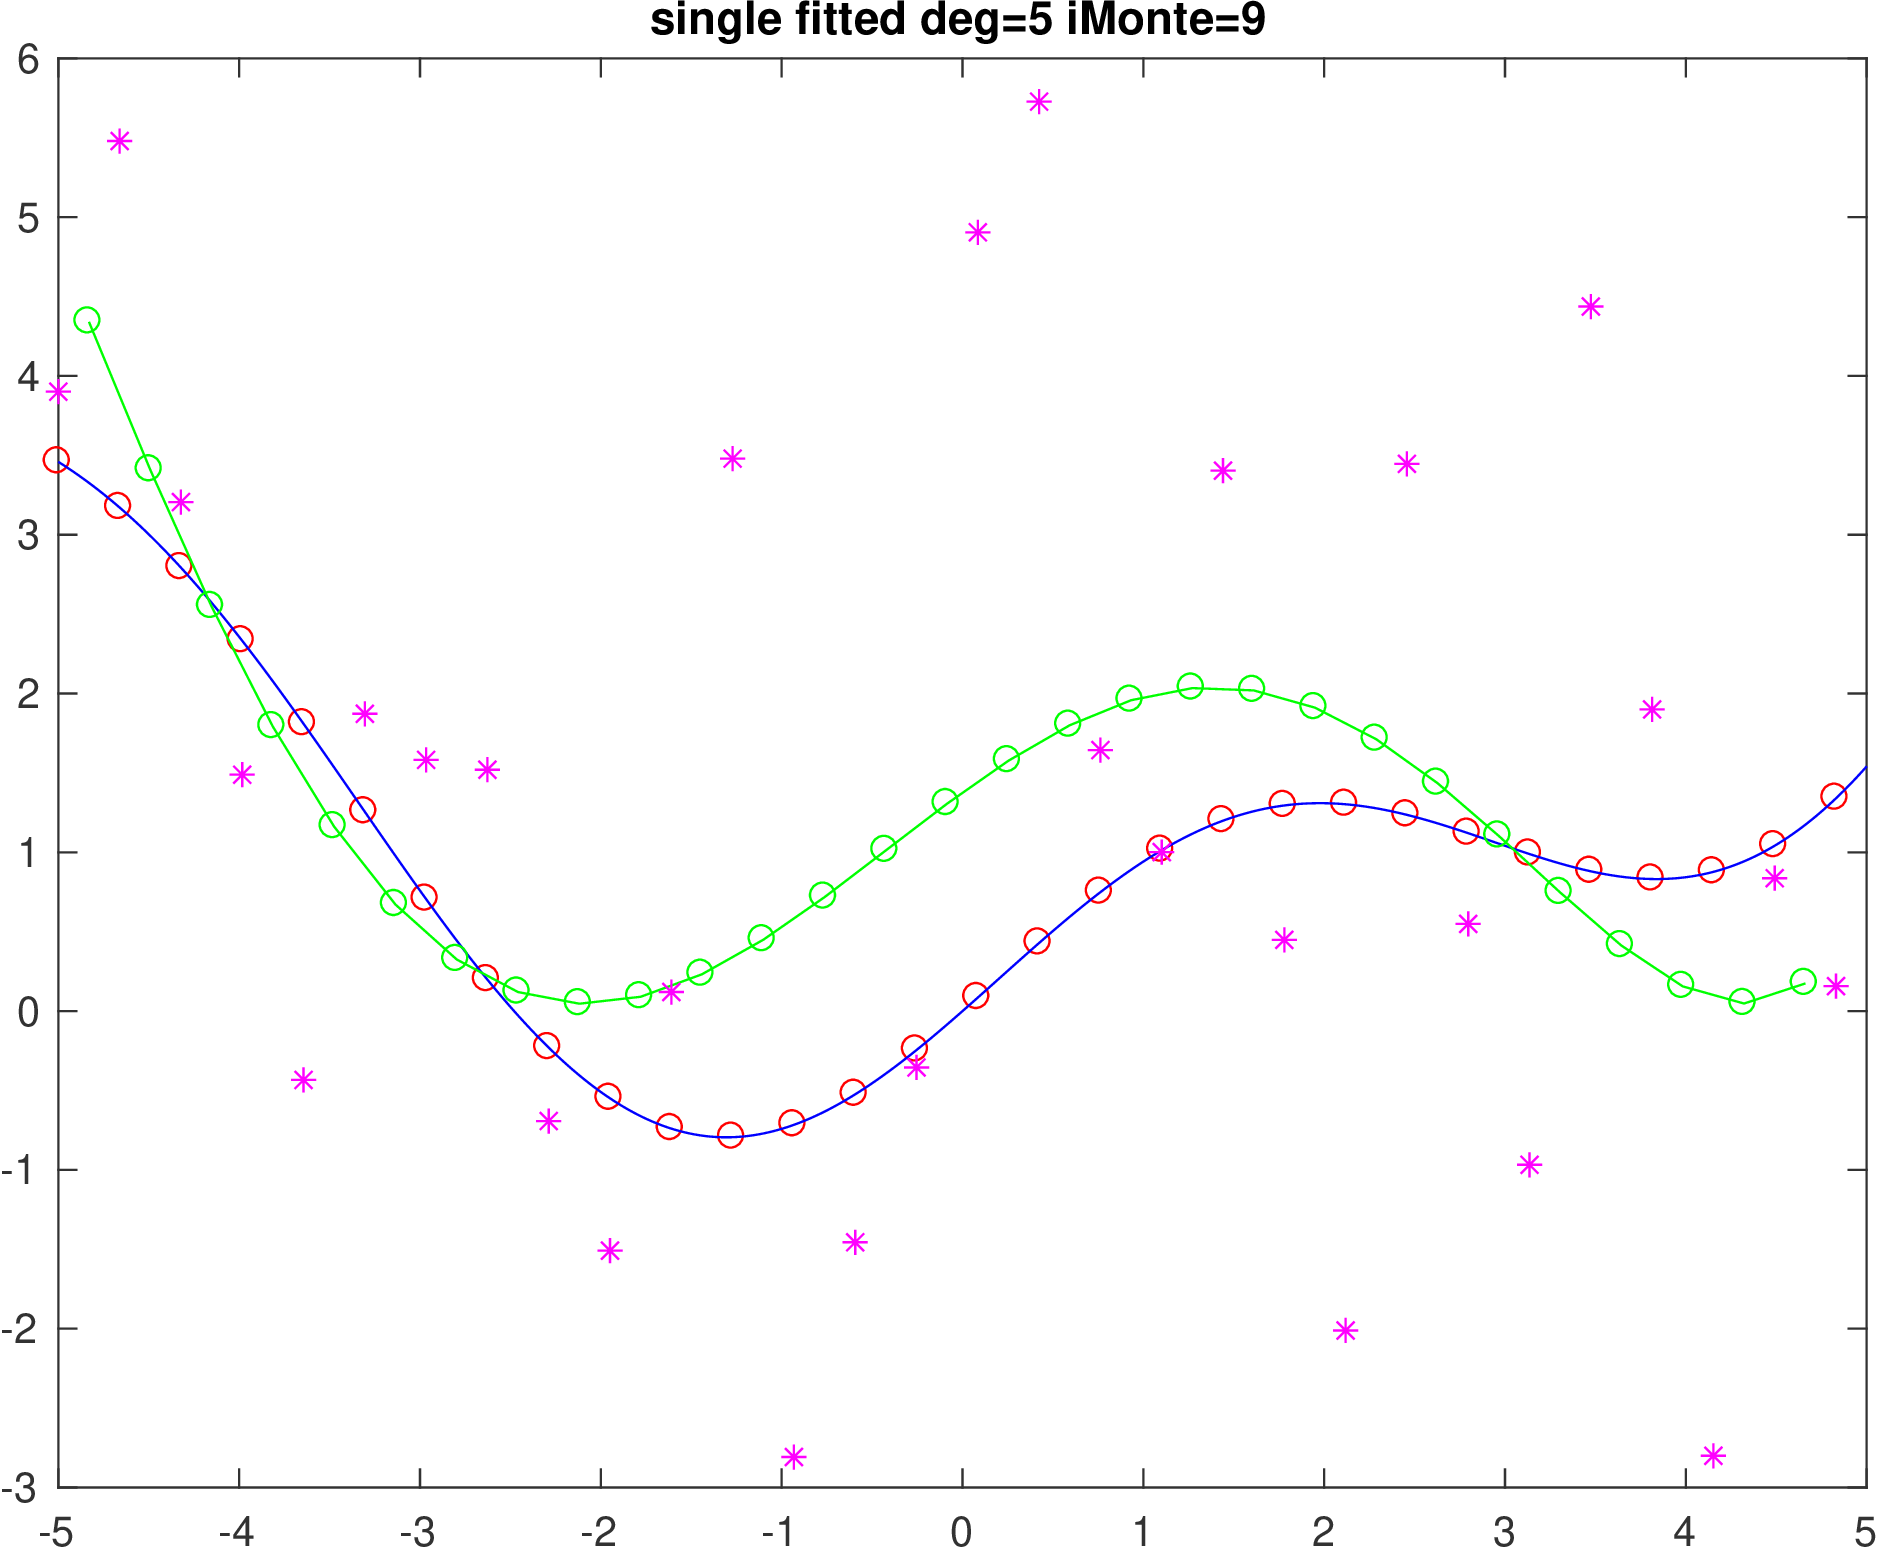
\includegraphics[scale=0.1]{single_poly_d_5_iMonte_9.png}
\end{figure}


\begin{figure}[h!]
\centering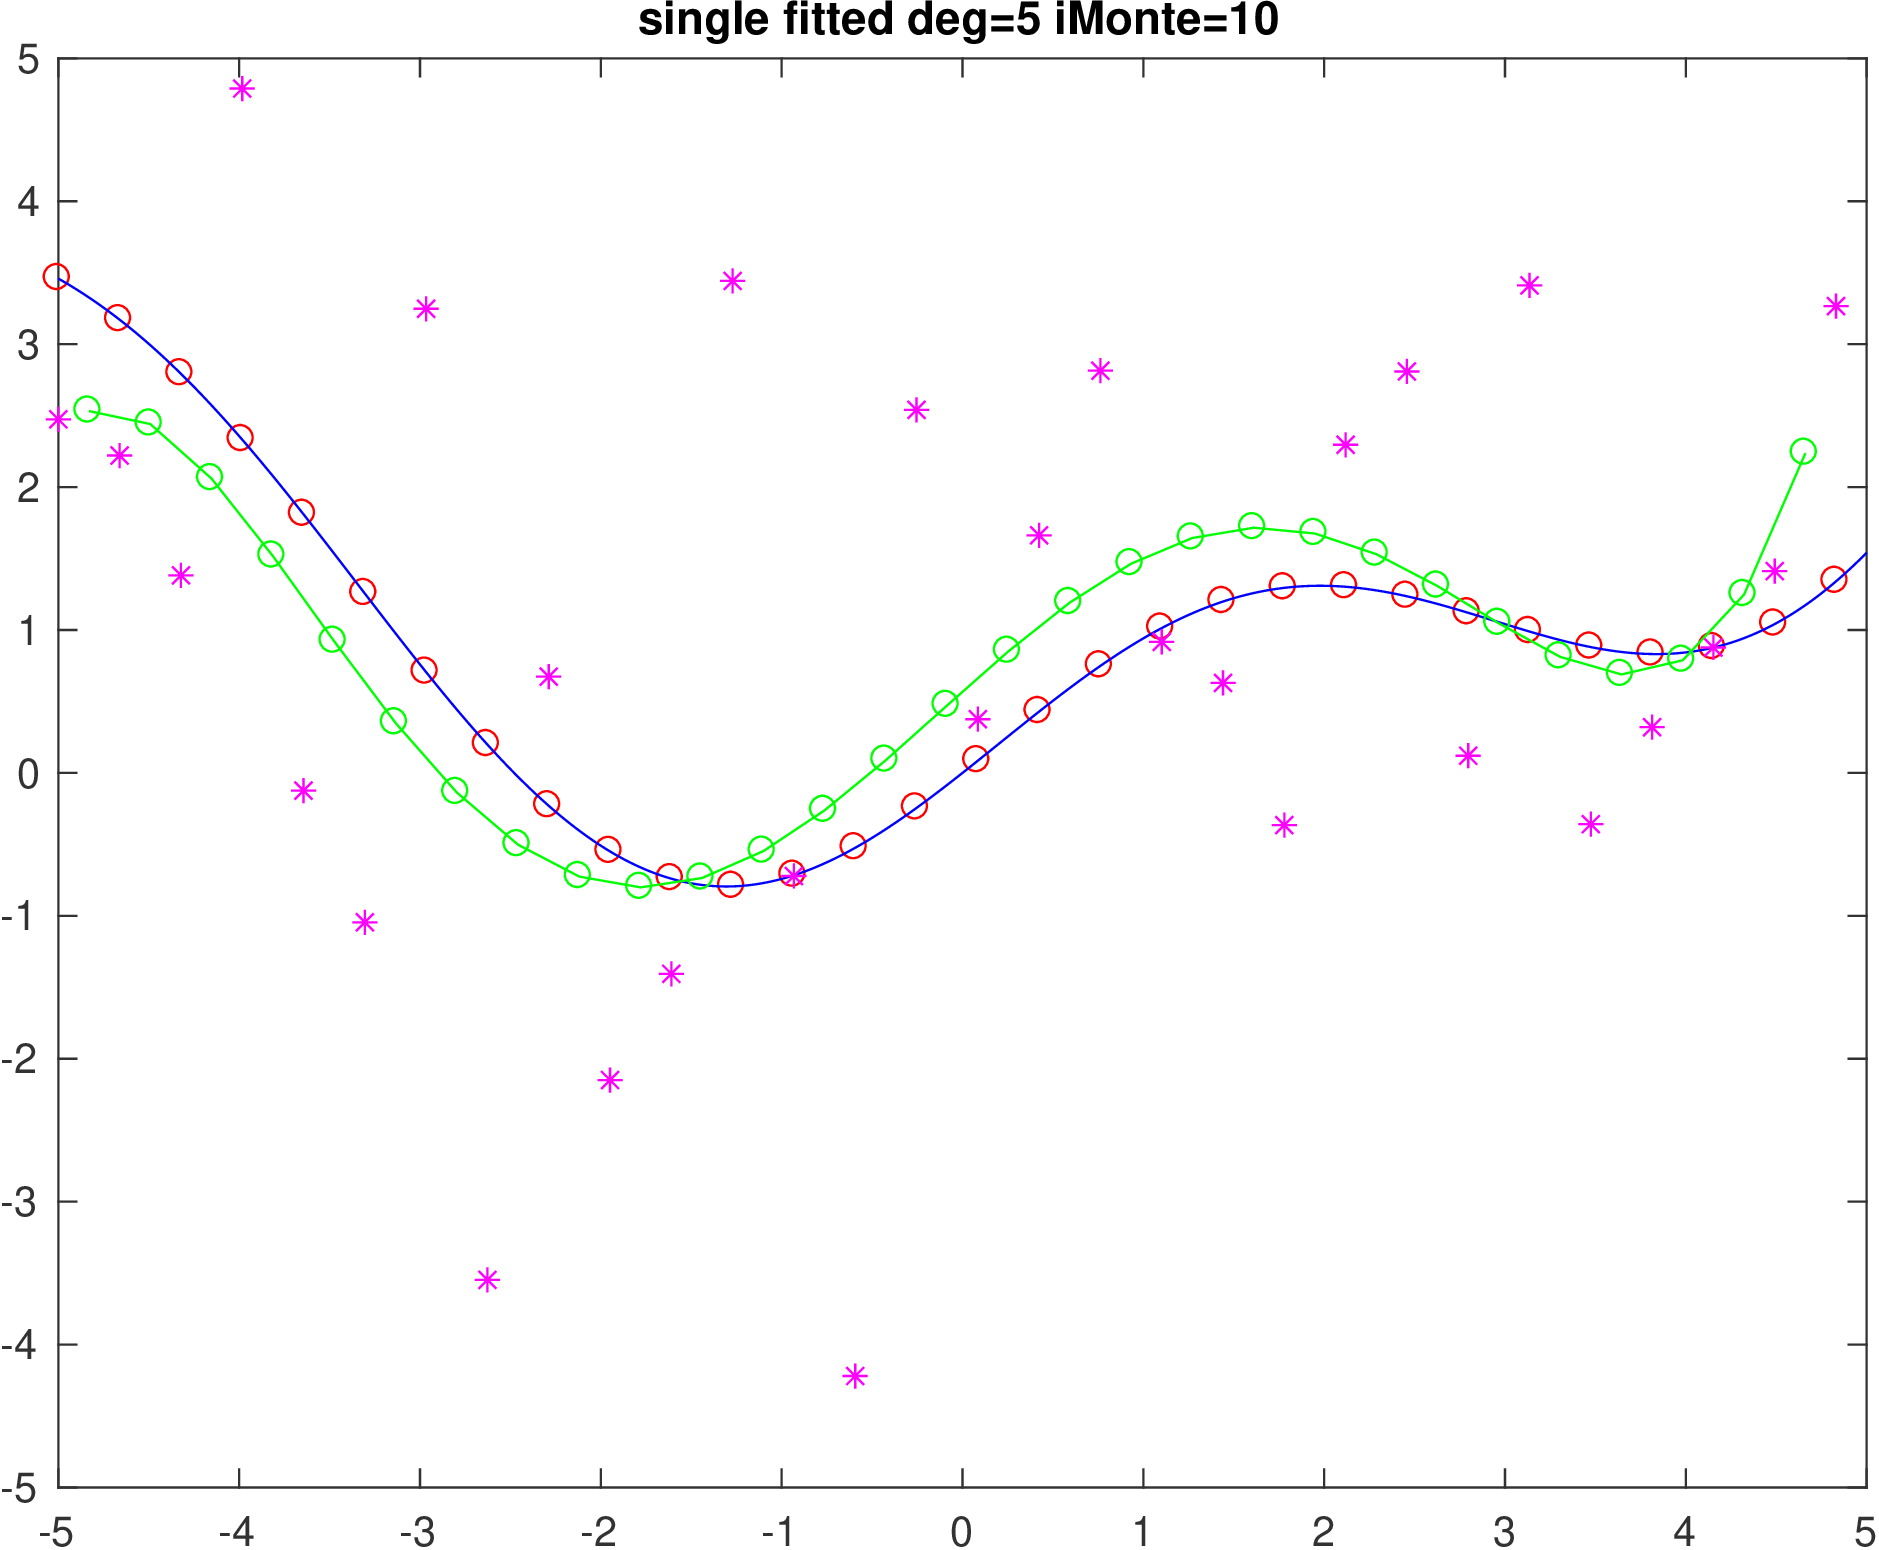
\includegraphics[scale=0.1]{single_poly_d_5_iMonte_10.png}
\end{figure}


\begin{figure}[h!]
\centering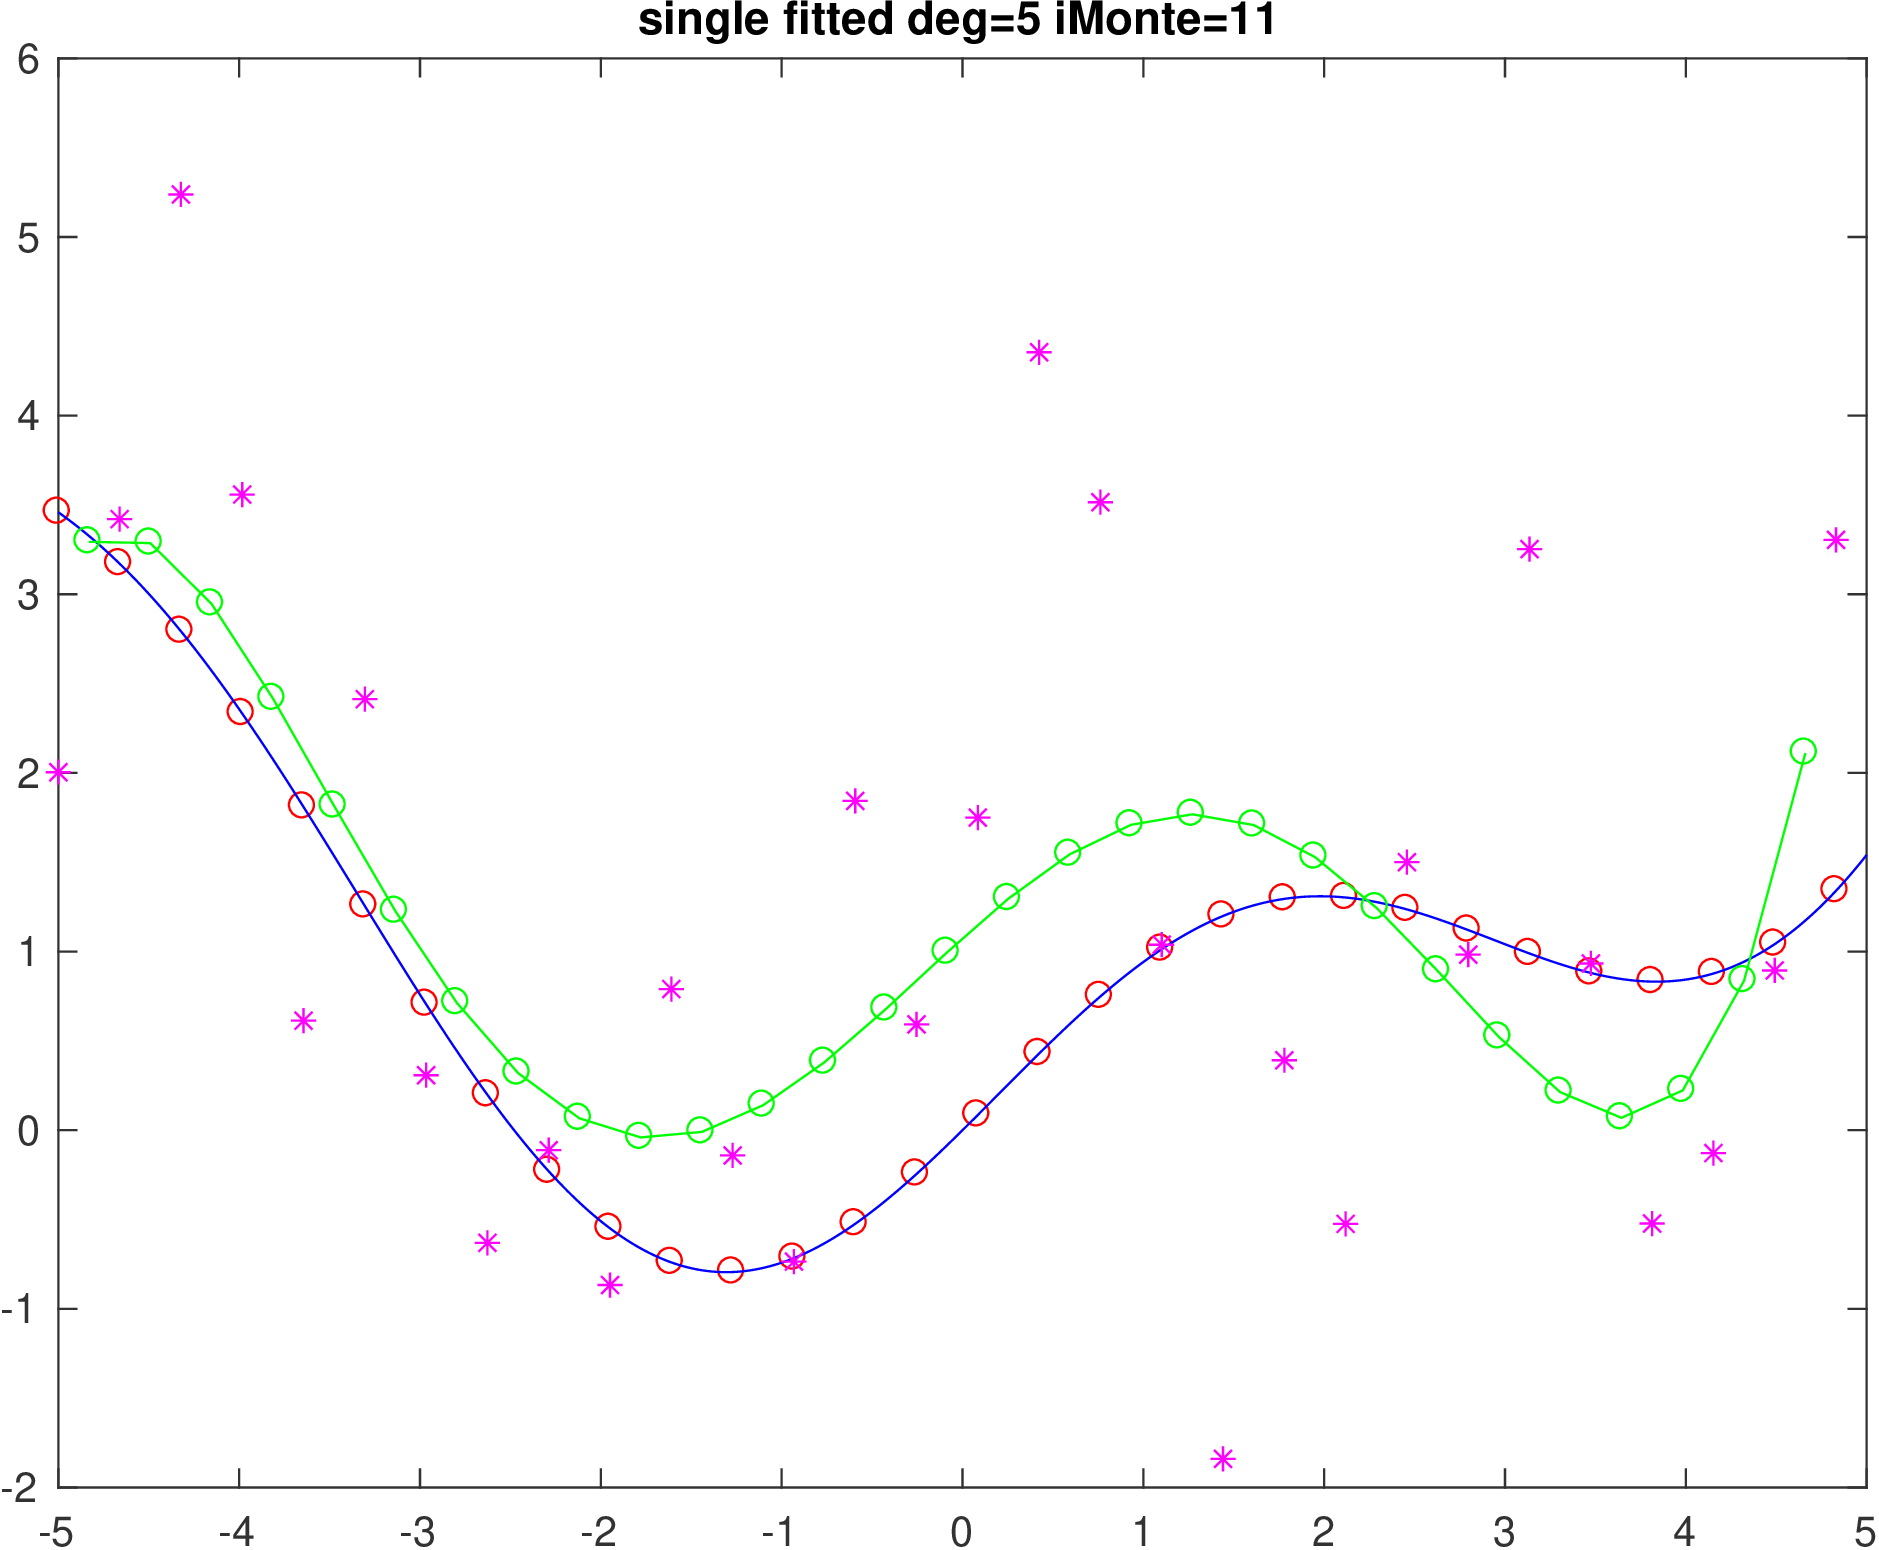
\includegraphics[scale=0.1]{single_poly_d_5_iMonte_11.png}
\end{figure}


\begin{figure}[h!]
\centering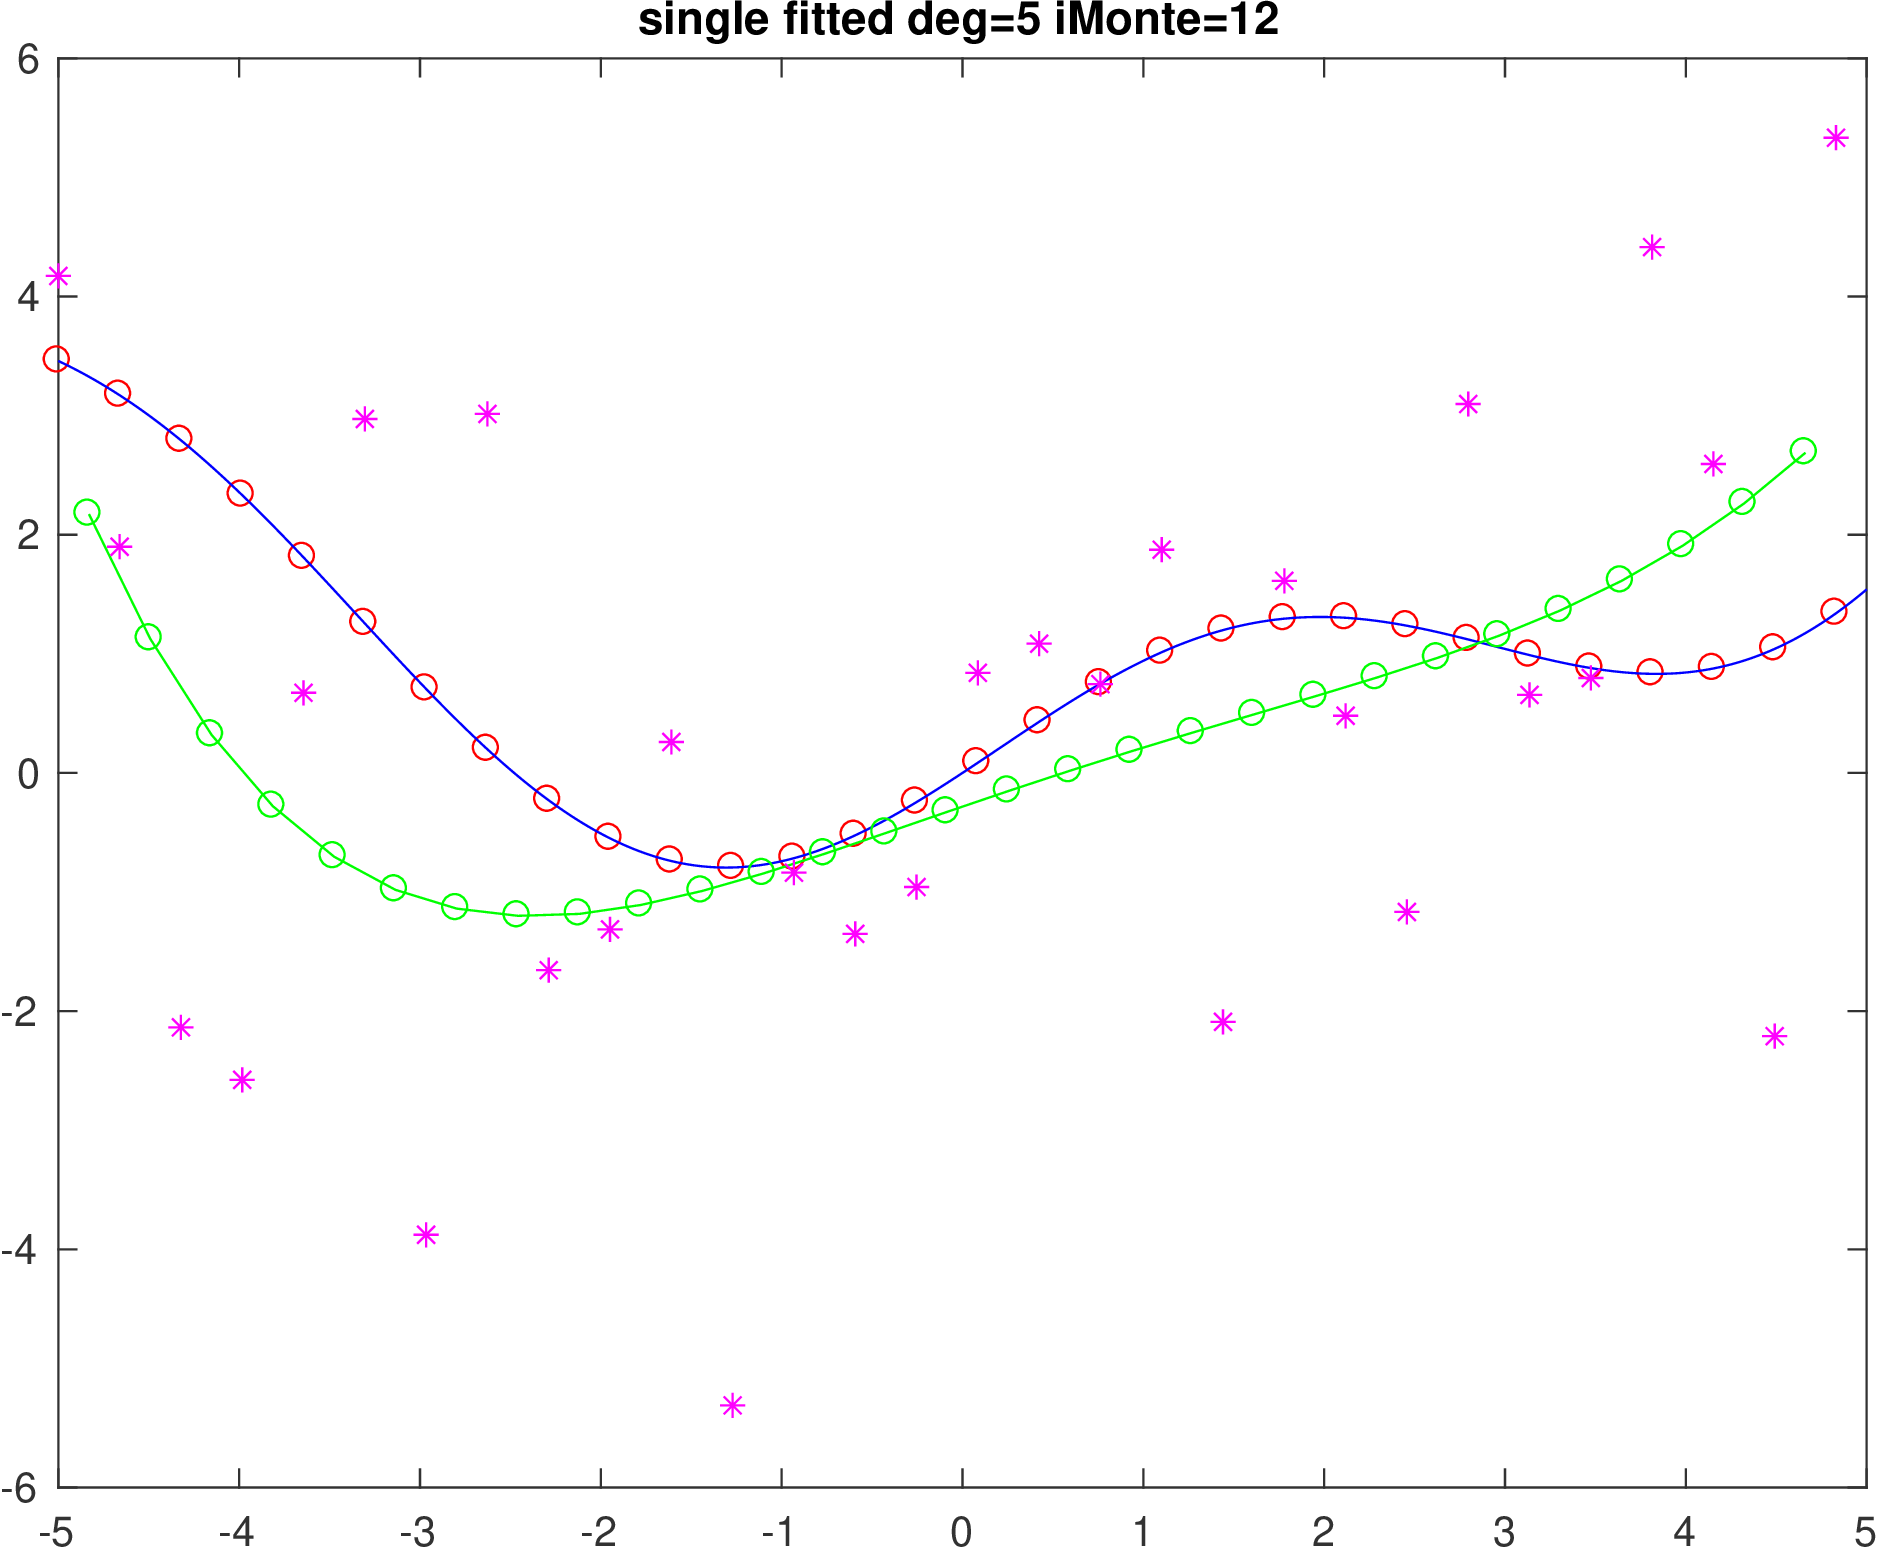
\includegraphics[scale=0.1]{single_poly_d_5_iMonte_12.png}
\end{figure}



\begin{figure}[h!]
\centering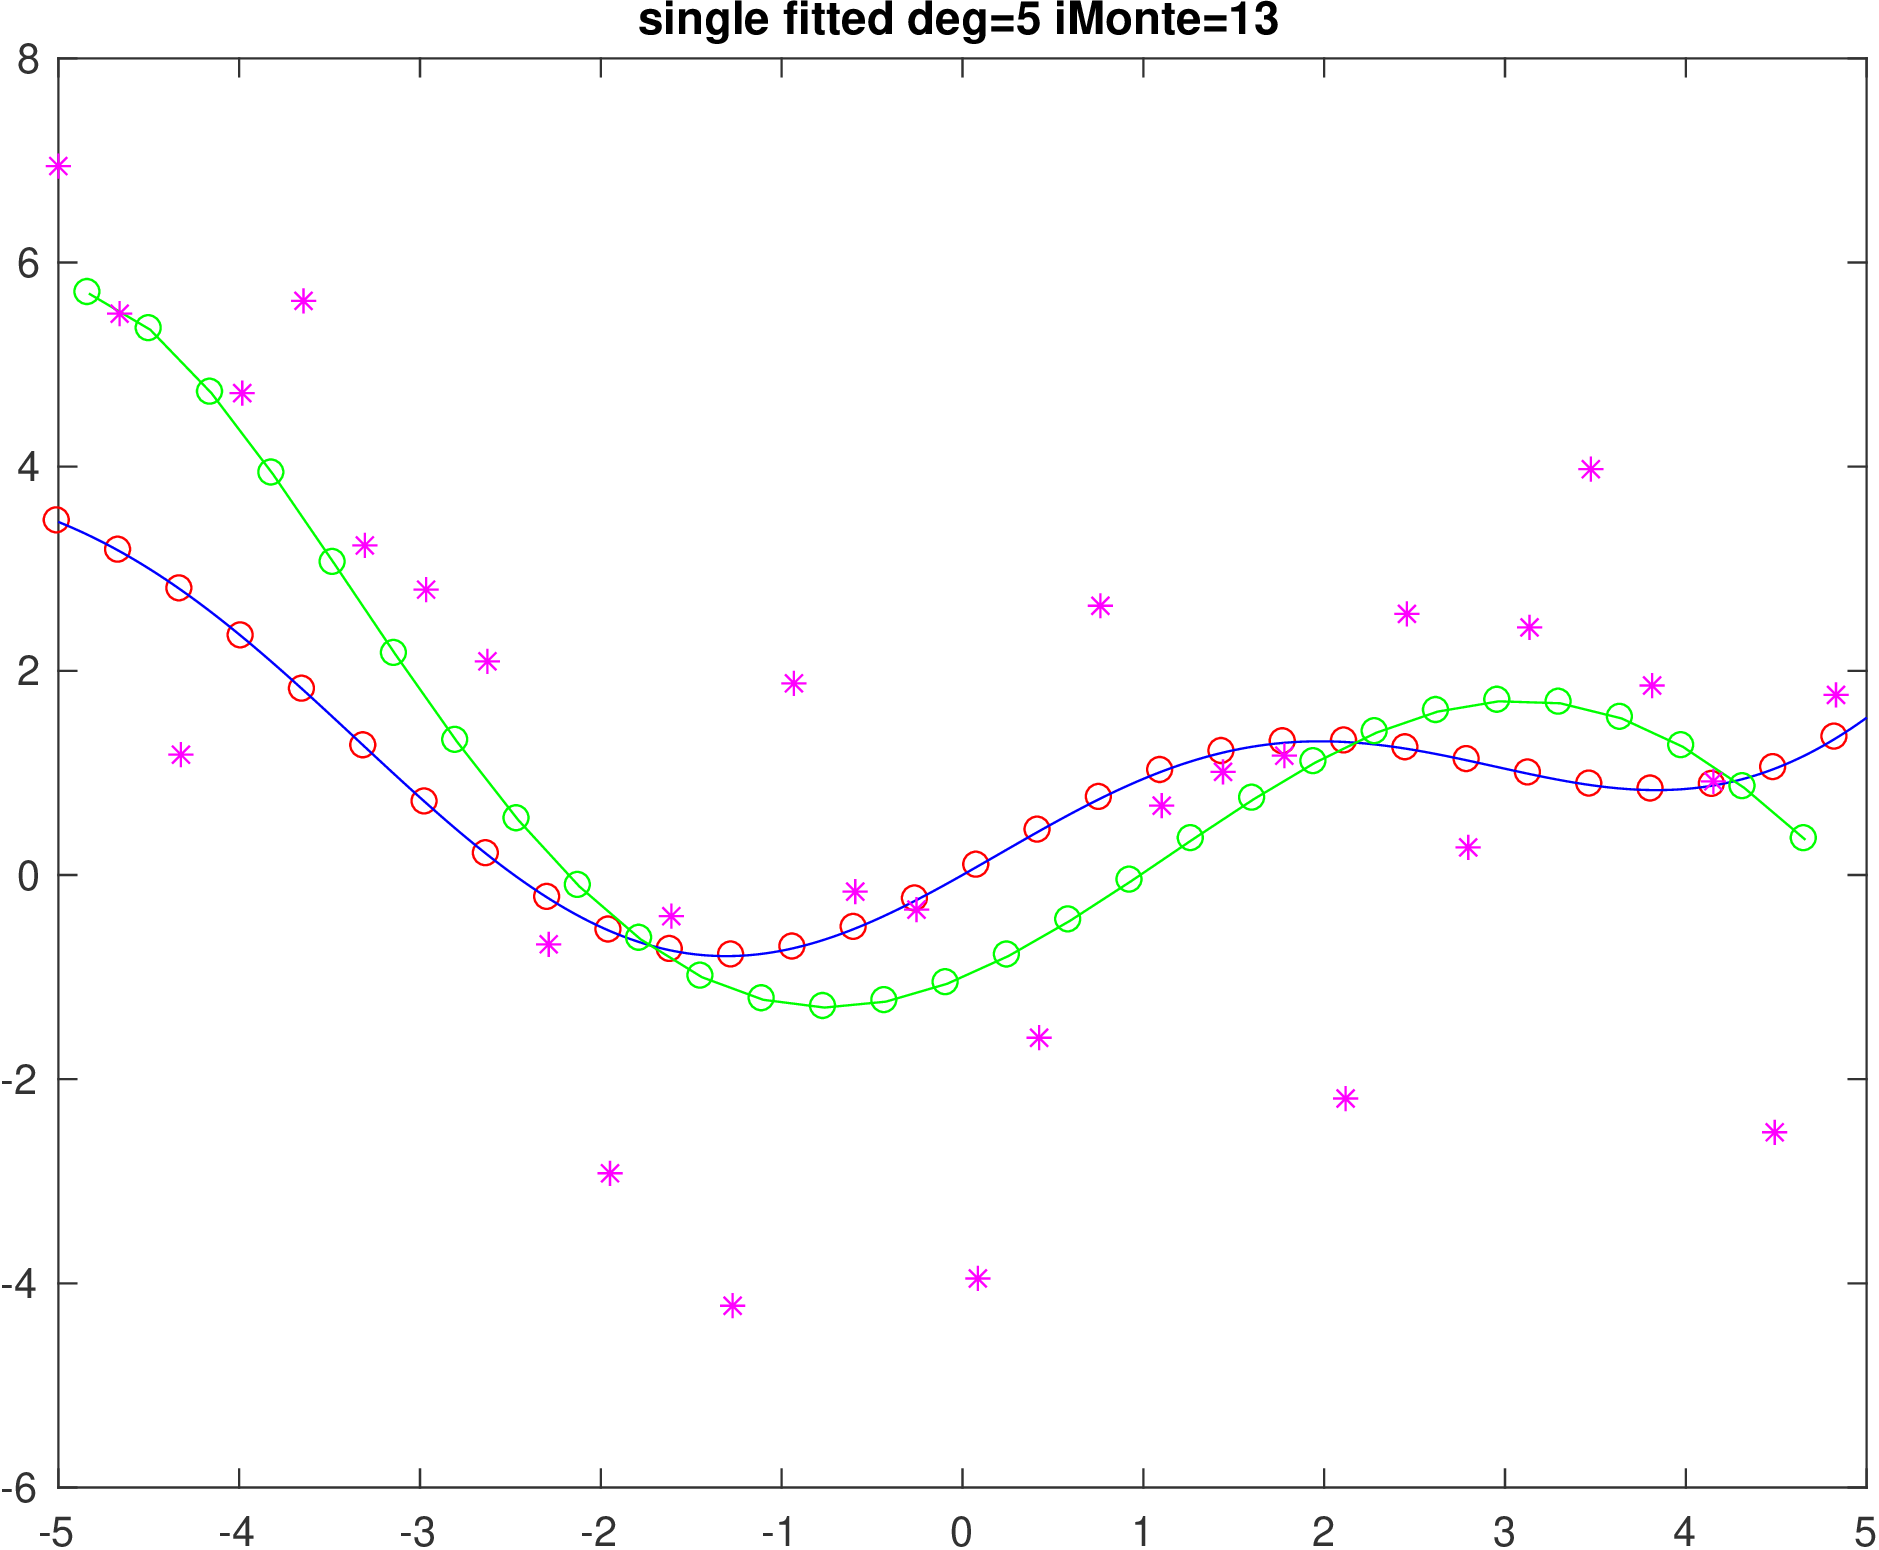
\includegraphics[scale=0.1]{single_poly_d_5_iMonte_13.png}
\end{figure}


\begin{figure}[h!]
\centering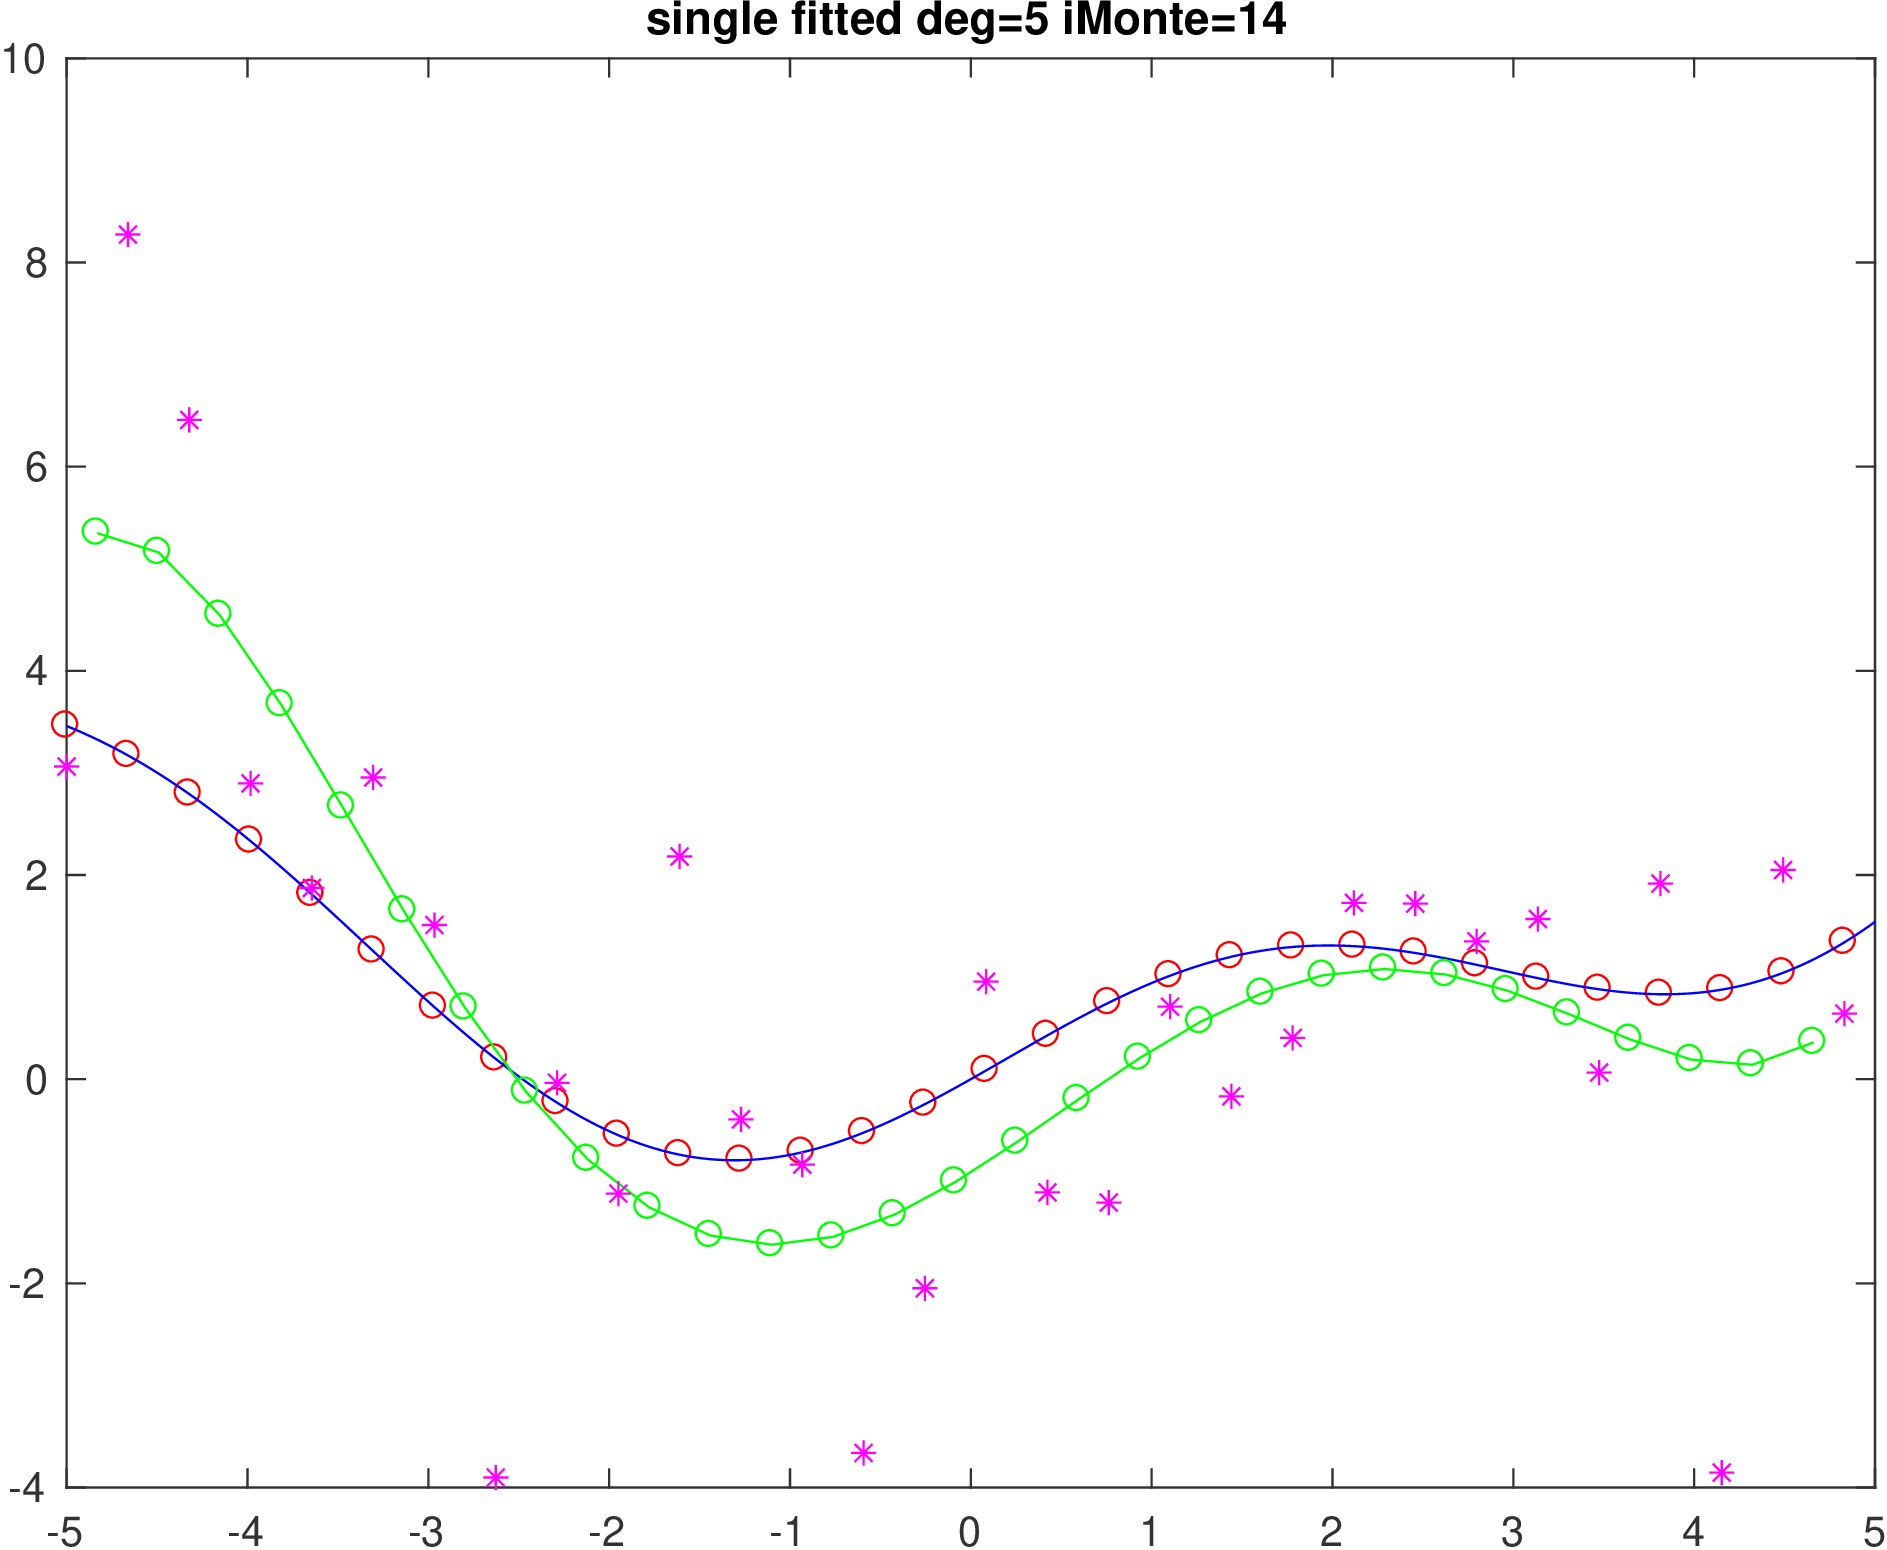
\includegraphics[scale=0.1]{single_poly_d_5_iMonte_14.png}
\end{figure}

\begin{figure}[h!]
\centering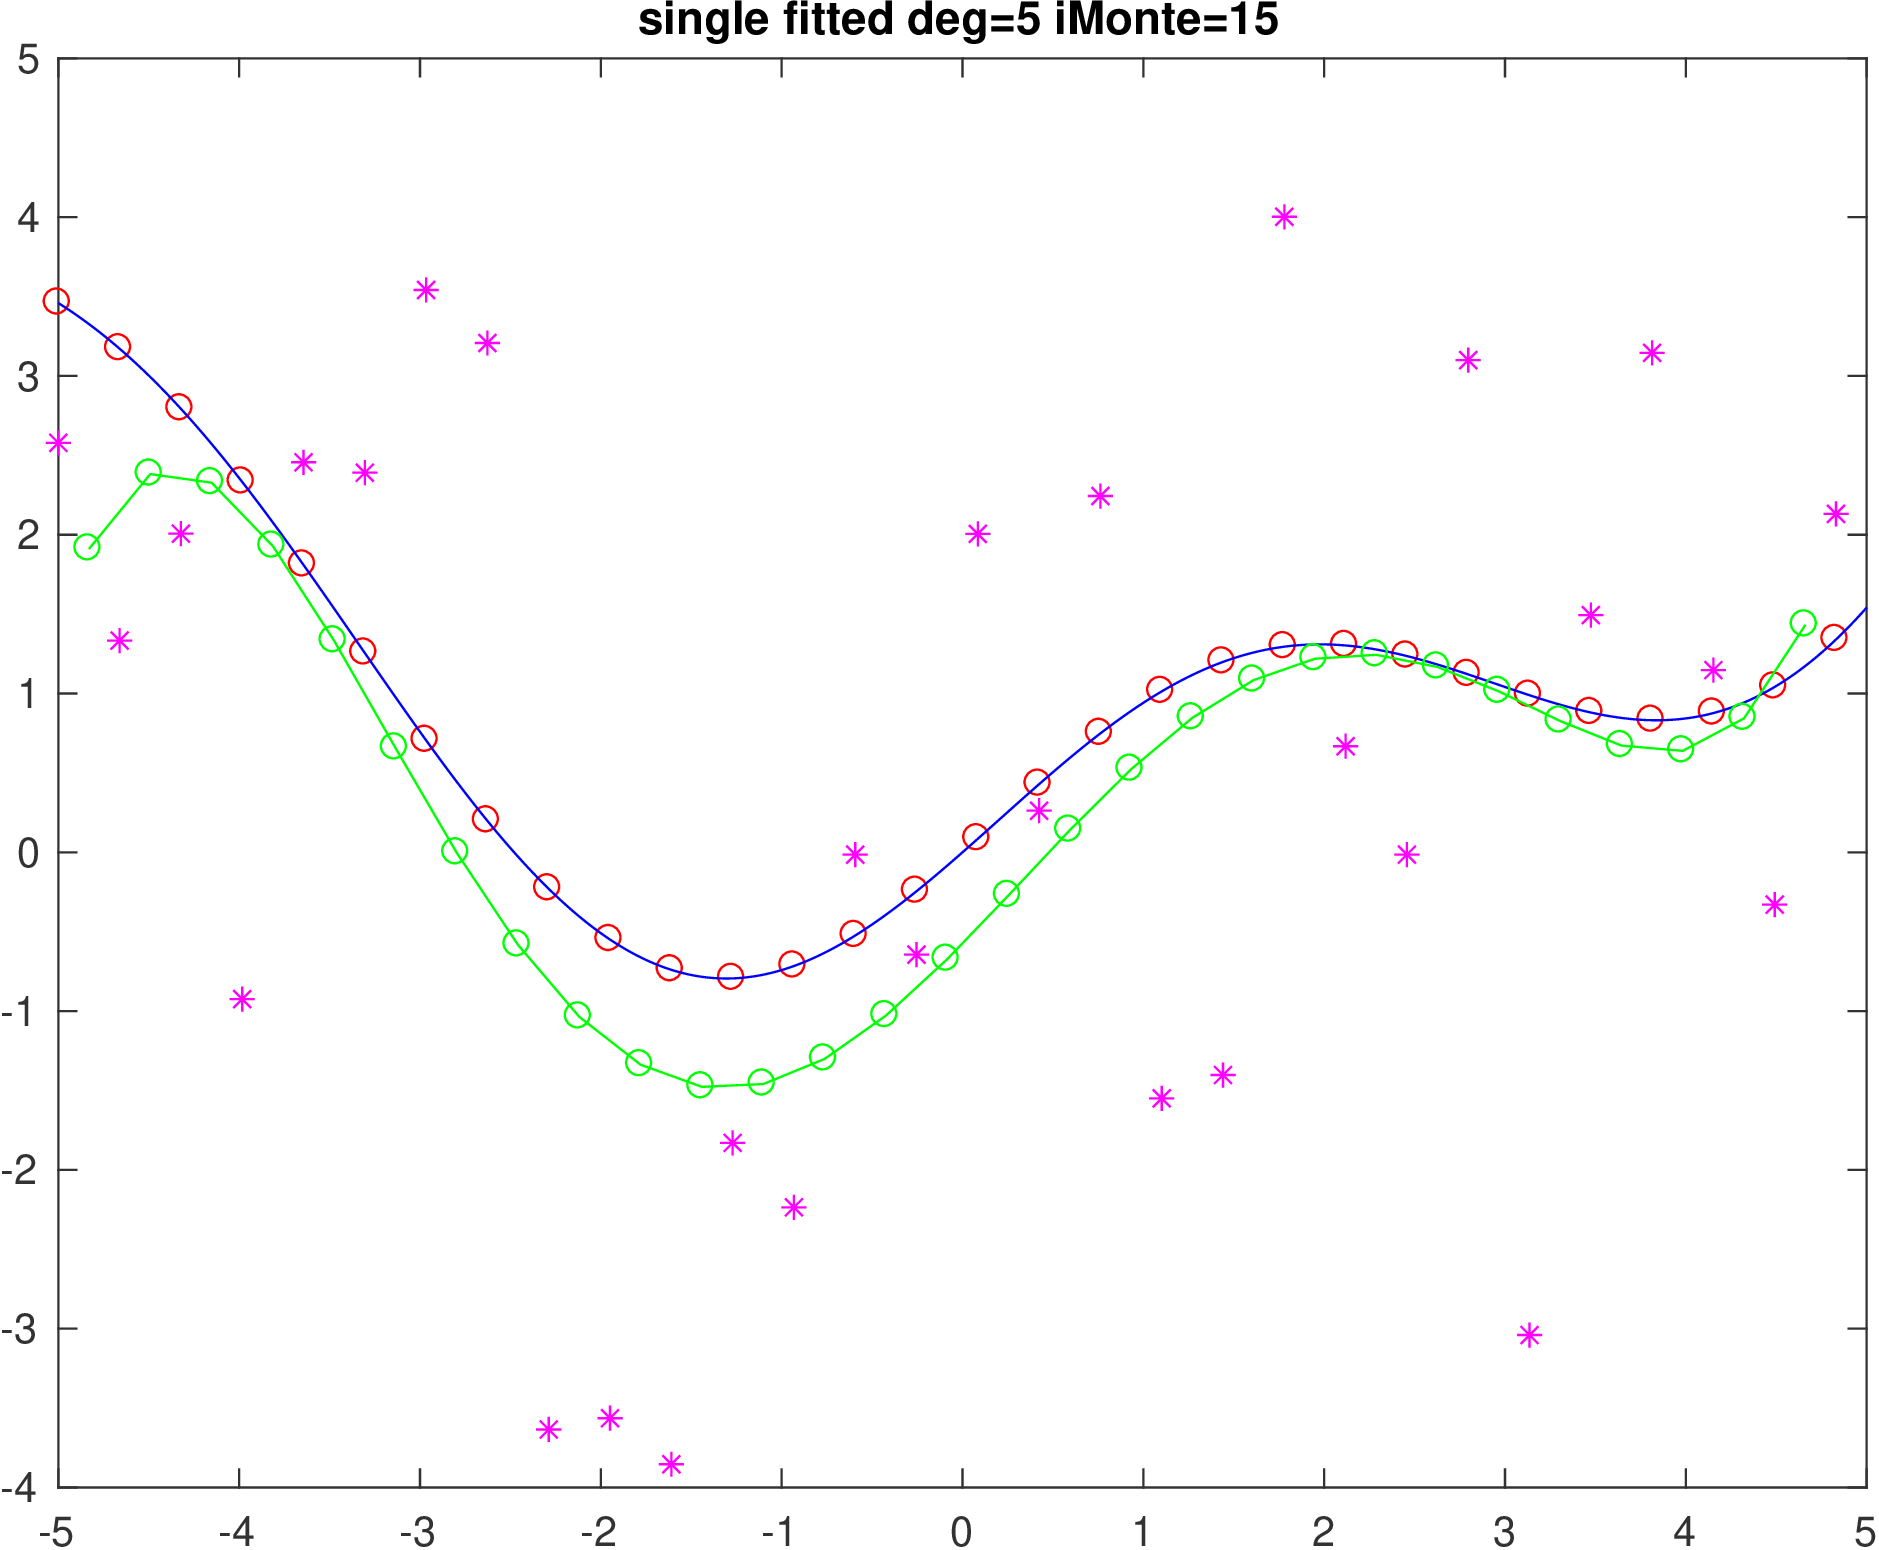
\includegraphics[scale=0.1]{single_poly_d_5_iMonte_15.png}
\end{figure}


\newpage


 Informally, {\bf Variance} is the variability in the learned prediction  rule $h_S$.
 Informally, the larger the hypothesis class, the higher the variance because the learning algorithm "chases after the noise" and "sees shapes in the clouds" - uses the freedom allowed by a larger hypothesis class
 and {\bf tries to describe the noise}


\subsection{Variance in linear model: Geometrical Interpretation}
Assume $y_i = \mathbf{x}_i^\Tr \mathbf{w}+z_i$, $i=1,\ldots,m$. To estimate $\mathbf{w}$ we project $\mathbf{y}$ onto $Im(X^\Tr)$.
Since the noise is i.i.d so, roughly speaking, it adds the same variability in all directions. 
The larger $Im(X^\Tr)$ inside the space $\R^m$, the more noise is  captured by the projection, and the more variability in $\mathbf{w}_S$ is seen.
 In the extreme case $m=d+1$ and $XX^\Tr$ invertible, $Im(X^\Tr)$ fills the whole space, so the projection does nothing. The noise has the largest possible influence on $\mathbf{w}_S$.
 We see that increasing training set size $m$ reduces the variance of $\mathbf{w}_S$

\newpage
\subsection{Bias-Variance Tradeoff}
What we have seen is a general phenomenon in machine learning:
      \begin{itemize}
               \item A small hypothesis class ("low model complexity") will generally  cause high bias and low variance
        \item A large hypothesis class ("high model complexity") will generally cause low bias and high variance
      \end{itemize}












\end{document} 